\documentclass[
  12pt      
  ,letterpaper
  ,center
  ,noupper
  ]{uconnthesis}
\ThesisLineSpacing{2}
\usepackage{graphicx}  % needed for figures
\usepackage{subeqnarray}
\usepackage{cases}
\usepackage{bm}        % for math
\usepackage{amssymb}   % for math
\usepackage{epstopdf}

\newcommand{\adag}{\ensuremath{a^{\dagger}}}
\newcommand{\bdag}{\ensuremath{b^{\dagger}}}
\newcommand{\cdag}{\ensuremath{c^{\dagger}}}
\newcommand{\ddagg}{\ensuremath{d^{\dagger}}}
\newcommand{\ket}[1]{\ensuremath{\left| #1 \right\rangle}}
\newcommand{\bra}[1]{\ensuremath{\left\langle #1 \right|}}
\newcommand{\braket}[2]{\ensuremath{\left\langle #1 \right|\left. #2\right\rangle}}
\newcommand{\mele}[3]{\ensuremath{\left\langle #1 \right|#2\left| #3\right\rangle}}
\newcommand{\dyad}[2]{{\ket{#1}\!\!\bra{#2}}}
\newcommand{\norm}[1]{\ensuremath{\left\| #1 \right\|}}
\newcommand{\abs}[1]{\ensuremath{\left| #1 \right|}}
\newcommand{\To}{\ensuremath{\rightarrow}}
\newcommand{\from}{\ensuremath{\leftarrow}}
\newcommand{\funE}{\ensuremath{\mathcal{E}}}
\newcommand{\beq}{\begin{equation}}
\newcommand{\eeq}{\end{equation}}
\newcommand{\bea}{\begin{eqnarray}}
\newcommand{\eea}{\end{eqnarray}}
\newcommand{\mbf}[1]{\ensuremath{\mathbf{#1}}}
\newcommand{\eq}[1]{{(\ref{#1})}}
\newcommand{\commentout}[1]{{}}
\newcommand{\idx}{{l}}
\newcommand{\half}{{\hbox{$\frac{1}{2}$}}}
\newcommand{\Kappa}{{\cal K}}
\newcommand{\bE}{{\bf E}}
\newcommand{\br}{{\bf r}}
\newcommand{\cbE}{\boldsymbol{\mathbf{\cal E}}}
\newcommand{\cbP}{\boldsymbol{\mathbf{\cal P}}}
\newcommand{\dip}{{\cal D}}
\newcommand{\bdip}{\boldsymbol{\mathbf{\cal D}}}
\newcommand{\G}{{\sf G}}
\newcommand{\bd}{{\bf d}}
\newcommand{\red}[1]{\textcolor{red}{#1}}
\newcommand{\blue}[1]{\textcolor{blue}{#1}}
\newcommand{\ja}[1]{\red{#1}}
\newcommand{\js}[1]{\textcolor{blue}{\textst{#1}}}

\begin{document}
\bibliographystyle{prsty}

\abstract{
\begin{center}
{ ABSTRACT}
\end{center}
At high density, dipole-dipole interactions between the atoms may have a major impact on light propagation in a dense gas. We have developed a classical-electrodynamics simulation to study the cooperative response of a near-resonant gas to light. We take into account the motion of the radiators using classical trajectories, including collisions with the walls of the container and atom-atom collisions, and describe the transition from homogeneously broadening to inhomogeneously broadened phenomenology.
}

\title{Cooperative Effects in the Optical Response of Dense Atomic Gases}
\author{Yi Li}
\date{2016}
\authorspreviousdegreelong{
  B.S., University of Science and Technology of China, Hefei, China, 2007 \\
  M.S., University of Connecticut, 2010
  }
\authorspreviousdegreeshort{M.S.}

\MajorAdvisor{Juha Javanainen}
\AssociateAdvisorA{Robin C\^ot\'e}
\AssociateAdvisorB{William Stwalley}

\dedication{
To ...
  }

\acknowledgements{
Firstly, I would like to express my sincere gratitude to my advisor Prof. Juha Javanainen. 
  }

\maketitle
\frontmatter
\tableofcontents
\listoffigures
%\listoftables

\mainmatter

\chapter{Introduction}

\section{Light scattering and cooperative effects}

Light scattering is the primary mechanism of physical observation. The state of the light field carries a great deal of information about the object with which the light has just interacted. A simple example is that one can tell the shape and color of an object by receiving the light scattered off its surface.

%Along with the exploration of the essence of light itself, the application of light as an indispensable tool to study the property of matter has achieved tremendous success since the dawn of modern science. 
 
With the development of physics, the models of light have kept getting more comprehensive. Beyond the simple ray model in geometrical optics, wave properties of light were introduced in the scope of physical optics. Later, within the framework of classical electrodynamics, light scattering could be explained satisfactorily. Examples include Rayleigh and Mie scattering. Both terms refer to discrete radiators in a liquid or gaseous medium, where each particle (e.g. an atom or a molecule) deflects the incoming light independently.

Assuming the light wavelength is $\lambda$ and the dimension of a particle is $D$, in the small particle regime ($D\ll\lambda$), Rayleigh scattering would be observed~\cite{Lilienfeld:04}. In a description as an elastic scattering process, each particle is treated as a classical dipolar radiator that oscillates at the same frequency as the incoming electric field and then re-radiates the field outward. In Rayleigh scattering, the relative intensity of the scattered light is proportional to $\lambda^{-4}$. This is the reason for the blue sky; the shorter the wavelength, the more scattering in the direction of our eyes.

When the size of the scattering particles is comparable to the wavelength ($D\sim\lambda$), the Rayleigh model breaks down. One can instead solve the Maxwell equations that describe a plane wave scattered by a homogenous sphere in terms of an infinite series of spherical harmonics. This solution describes Mie scattering~\cite{1908AnP...330..377M}.  There are some remarkable features about Mie scattering that make it different from Rayleigh scattering. For example, the intensity of the scattered light is generally higher in the forward direction than in the backward direction; the larger the particle, the more of the light is scattered in the forward direction. Rayleigh and Mie scattering have features similar to the light scattering processes in dense gases that we study in this dissertation.

%The optical property of a medium hinges on the nature of light-matter interactions that take place inside it.

In many cases light scattering is an important aspect of the optical response of a material sample to light. For example, light attenuation inside a medium of independent radiators may often be understood as scattering of light away from the incident beam. The relative intensity of the transmitted light may, of course, always be written in terms of the optical thickness (optical density, optical depth) $D$ of the sample as
\bea
I_{out}=I_{in}\,e^{-D}.
\label{BEER'S_LAW}
\eea
In a common case the optical thickness is given by the thickness of the sample $h$, the total cross section of light scattering from the radiators $\sigma$, and the density of the scatterers $\rho$ in the form $D=\sigma\rho h$. This is known as the the Beer-Lambert law. It is, for instance, one of the theoretical bases of absorption imaging, a commonly used technique to extract information about the sample in cold-atom experiments. 

%Another possibility that this law fails could happen when the light is quite intense, the nonlinear optical processes will then alter the bulk property of the sample.


%(cooperative effects; time domain: superradiance; frequency domain: CLS)~\cite{PhysRevLett.112.113603}

%(mean-field theory; continuous medium; independent radiators; interacting radiators.)

%(light-matter interaction: from simple to complex: classical scattering, attenuation, fluorescence, polarization of a medium, ensemble-light interfaces)

%The Beer-Lambert law does not distinguish microscopic mechanisms of the light attenuation, such as absorption and scattering by atoms in the sample. Moreover, it also neglects all the other attributes of the light except the intensity. 

%\section{The role of light in modern physics}

In the era of modern physics, the role of light scattering is even more important. Of course, light is still a natural and feasible way of probing the state of the material with which it interacts. For example, at the time of the first realizations of Bose-Einstein condensates~\cite{Anderson14071995,PhysRevLett.75.3969}, the properties of light scattering from BECs were widely discussed~\cite{PhysRevA.43.6444,PhysRevA.51.3896,PhysRevA.52.3033,PhysRevLett.71.1339}  and a number of proposals for employing light scattering to detect BECs were raised. Characteristic details in the line shape for light scattered from BECs were predicted for different configurations~\cite{PhysRevLett.72.2375,PhysRevA.50.R3565,PhysRevLett.75.1927,PhysRevLett.76.1774,PhysRevA.54.R2543}. Though much trickier than one might wish, it is in principle possible to verity the existence of a Bose-Einstein condensate by spectral measurements of the scattered radiation from an atomic sample. Another example of theoretical proposal is probing quantum statistics of atoms in an optical lattice by light scattering~\cite{PhysRevA.76.053618}. In practice, for instance, an experiment that uses light scattering to determine the relative phase of two Bose-Einstein condensates has been carried out~\cite{Saba25032005}.

Furthermore, in the context of quantum measurement theory, light scattering is likely to be a common probe for nondestructive measurements~\cite{RevModPhys.68.1}, continuous observation, and feedback control. For example, a nondestructive measurement to probe the quantum state of a 1D Bose gas using off-resonant light scattering was proposed\cite{PhysRevLett.107.270403}. Another example is monitoring continuously and non-destructively the number of atoms in a Bose-Einstein condensate by light scattering as the atoms oscillate back and forth between two sides of a double-well trap\cite{NJP.JJ}.

From an even broader perspective, understanding light-matter interactions, including light scattering, is critical for the work on controlling quantum systems, which in turn opens the way for practical techniques such as quantum computer and quantum communication. One approach to control the light-matter interaction is cavity quantum electrodynamics (cavity QED)~\cite{0034-4885-69-5-R02}. In general, a weak coupling between the cavity field and the atoms leads to modifications of the internal state of the atoms. In the strong coupling case, atoms and photons are entangled, this being the basis for many interesting applications.  Many fascinating experiments have been performed on  phenomena such as  photon blockade~\cite{photon_blockade}.

Another way to control light-matter interactions is to interface light with an atomic ensemble. To be specific,  optically thick atomic ensembles can be efficiently interfaced with light so that the quantum features of light-matter interactions are preserved~\cite{RevModPhys.82.1041}. In recent years, this approach has become a very active area of research. Nonetheless, developing a thorough understanding of the optical response of a dense atomic ensemble to light is a challenging task. Suppose that light scatters repeatedly  between the atoms. Comparing to ensembles of independent or weakly correlated atoms, strong correlations between the atoms induced by multiple scattering may dramatically alter the way the light and the atoms interact.  In effect, the entire material sample may respond cooperatively to light.

Experimentally, the cooperative effects in light scattering have been studied intensively in recent decades.  Superradiant Rayleigh scattering from a Bose-Einstein condensate was studied\cite{Inouye23071999,PhysRevLett.83.5202,PhysRevA.62.063615} and cooperative Mie scattering from an ultracold atomic cloud was observed\cite{PhysRevA.82.011404}. Moreover, recent experiments demonstrated that the density fluctuations in the atomic cloud tend to suppress cooperativity\cite{PhysRevLett.104.183602}, and that the cooperativity generates a shift of the optical transition frequency that depends on the density and geometry of the atomic sample\cite{PhysRevLett.108.173601}. The cooperative effects also lead to the phenomenon that the radiation pressure of a laser beam would be modified by the scattered photons\cite{Eur.Phys.J.D.58.1}.

The importance of light-matter interaction calls for more insights into cooperative effects in a medium when light passes through. However, analysis of cooperative response of a dense medium is a challenge because of the combination of the strong short-range divergence $(1/r^3)$ and the long range $(1/r, $ for radiating atoms$)$ of the dipolar field and the ensuing dipole-dipole interactions. The literature is replete with approximations\cite{FRIEDBERG1973101}. In this dissertation we promote an alternative approach, numerical simulations of classical light propagating in a medium of classical induced dipoles. Starting from quantum field theory for both atoms and light, it has been shown\cite{PhysRevA.55.513} that such an approach is valid and gives the same results as the full quantum theory basically when photon recoil and saturation of the atoms may be neglected. We develop software objects in C++ to carry out classical light propagation studies in an (in principle) arbitrary collection of classical dipoles, and use them to understand the emergence of the cooperative effects in common geometries. Our early simulations of inhomogeneously broadened samples with stationary atoms have sharpened and modified traditional theory of cooperative effects. The more recent simulations with moving atoms verify existing theoretical predictions and reveal new features in spectroscopic observations that can also be categorized as cooperative.


\section{Outline}

In Chapter 2, the theoretical basis of the research is reviewed. A fundamental notion of quantum optics, the semi-classical theory of the interaction between a two-level atom and a classical light field, is briefly reviewed. The polarizability of an atom regarded as a damped two-level system is particularly emphasized. Additionally, we introduce the local-field corrections,  Clausius-Mossotti relation, and the Lorentz-Lorenz formula in this chapter. These are critical in discussions of cooperative effects that we will have later in the dissertation.

Chapter 3 qualitatively describes two typical of cooperative effects in a system of strongly interacting dipoles. While observing the spontaneous emission from a dense sample, the emitted field intensity is much stronger and the duration of the pulse is much shorter than would be the case for  independent atoms. We recap Dicke's pioneering work on superradiance in this chapter. On the other hand, in the frequency domain, besides the generic Lorentz-Lorenz shift  in the absorption spectrum brought on by the local-field corrections, another type of shift called collective Lamb shift can be observed in a dense sample because atoms are correlated with the virtual photons of the QED vacuum. We emphasize superradiance and CLS here as they are phenomena that repeatedly come up in our research. In the last section of this chapter, the exact definition of cooperativity is discussed before we embark on further calculations and simulations.

The primary technique of our research, classical-electrodynamics simulations, is introduced in the beginning of Chapter 4. After a discussion of the validity and scope of application of our simulations, we firstly solve the problem of light scattering from a single atom and a two-atom system. Then detailed calculations are carried out on a hypothetical cloud of independent radiators whose spatial distribution is Gaussian.  When dipole-dipole interactions are added to this Gaussian cloud, we find from the simulations that the cooperative effects in emission intensity show up at an unexpectedly low density. The simulation of the Gaussian cloud is followed by a more realistic simulation of a dense gas in a circular disk container. The most important technical addition in this instance is an artificial inhomogeneous broadening of the atomic sample. We find that such a broadening in the system of discrete radiators leads to a close agreement with the traditional predictions of the collective Lamb shift.

In Chapter 5, an important feature is added to the simulations: the motion of the atoms. When atom-atom collisions, collisions of the atoms with the walls of the container,  and the free flight in between are taken into account, the model becomes more comprehensive and hence displays more intriguing phenomena. Both a semi-analytical treatment of a single atom and the simulations of independent atoms show a narrow resonance peak in the absorption spectrum. This is a clear signature of Dicke narrowing due to atomic collisions. Again, things are different when the atoms are strongly correlated. When we introduce the dipole-dipole interactions between the atoms, the dependence of the collective Lamb shift on sample thickness appears to follow the traditional predictions. However, the width of the resonance becomes another signature of cooperativity.  A transition from a clearly Dicke narrowed peak in a dilute gas to a greatly broadened peak in a optically dense sample is observed in the simulations.

Finally, we summarize our work in Chapter 6. We also survey possible future directions for related studies.


%Apparently, the success of classical scattering theories such as Rayleigh and Mie scattering results from the fact that the model with classical dipoles is much more realistic than the continuous-medium model. 

%However, it doesn't end here. The fundamental principles that rule the real world is quantum, not classical, including both sides of the light-matter interactions. Quite a lot of optical phenomena could only be interpreted by quantum theories. A prime example is the spontaneous emission of atoms.

%A well known semi-classical description of spontaneous transitions is given by the Einstein A and B coefficients. In this framework, the atom is quantized but the electromagnetic field is not. 

%In an ordinary fluorescence experiment of two-level atoms, assume that the sample has $N(0)$ atoms initially prepared in the upper level, then the number of excited atoms at time $t$ is given by
%\bea
%N(t)=N(0)e^{-At}=N(0)e^{-\Gamma t}=N(0)e^{-t/\tau},
%\eea
%where the Einstein A coefficient is just the spontaneous decay rate $\Gamma$, which in turn equals to the reciprocal of the lifetime $\tau$.

%The fundamental mechanism of spontaneous transition can only be explained by a quantized electromagnetic field. In quantum electrodynamics, the spontaneous transition in free space is a consequence of the interaction between the atom and the QED vacuum. In the dipole approximation, the rate of spontaneous emission $\Gamma$ is given by
%\bea
%\Gamma=\frac{k^3d^2}{3\pi\hbar\epsilon_0}.
%\eea
%Given a sample composed of independent atoms, due to the infinite number of degrees of freedom of the electromagnetic field, the radiation pattern of the spontaneous emission would be essentially isotropic.

%In summary, if the constituent particles are treated as independent radiators, i.e., the sample is sufficiently dilute so the interaction between particles is neglected, the eventually observable electromagnetic field from a sample can be predicted as a simple superposition of the post-interaction fields (photons) from all the particles in the sample. The interacting field can be vacuum or not.







\chapter{Semiclassical Theory of Interaction between Two-level Atoms and Classical Light}

\section{Electrodynamics of a polarizable medium: Local-field correction and Clausius-Mossotti relation}
\label{LFC}

In a dense liquid or gaseous medium, the electric field on an individual atom\footnote{From now on we generically refer to a dipolar radiator in a medium as an ``atom'', even if many general results apply to any particles with dipole moments.} will be influenced by the fields from the other atoms. Conventionally, a mean-field theory (MFT) that represents the dipole moments of the atoms as a continuous polarization is used to study the field on the atom.  Consider the ``spectator'' atom in such a medium~\cite{feynman}. The field acting on the atom $\cbE_{loc}$ can be approximated by the field in a small spherical hole centered at the position of the atom. Imagine that this spherical hole is formed by ``scooping out'' a sphere of the polarized material, let $\cbE$ be the average field in the medium, and $\cbE_{sphere}$ be the field inside the sphere if it were there. Because of the superposition principle we have
\bea
\cbE=\cbE_{loc}+\cbE_{sphere}.
\label{E_MEAN}
\eea
Given a sphere small enough to be uniformly polarized,  the field inside the sphere is also uniform and has the value
\bea
\cbE_{sphere}=-\frac{\cbP}{3\epsilon_0},
\label{E_SPHERE}
\eea
where  $\cbP$ is the polarization.

Combining Eq.~\eq{E_MEAN} and Eq.~\eq{E_SPHERE}, we obtain the expression of the local field at the position of the atom in the medium as
\bea
\cbE_{loc}=\cbE+\frac{\mathbf{\cbP}}{3\epsilon_0}.
\label{LOCAL_FIELD}
\eea
The term $\cbP/3\epsilon_0$  is referred to as local-field correction. We will invoke this concept in later chapters when we discuss the interpretation of the results from approaches that go beyond MFT.

For now, we can take one more step forward. Assume $\alpha$ is the polarizability of each individual atom, so that in the field $\cbE_{loc}$ an atom develops the dipole moment $\bd = \alpha \cbE_{loc}$.  Taking the number density of the medium to be $\rho$, we have
\bea
{\cbP}=\rho\bd=\rho\alpha\cbE_{loc}=\rho\alpha\left(\cbE+\frac{\mathbf{\cal{P}}}{3\epsilon_0}\right).
\label{POLARIZATION}
\eea
The susceptibility $\chi$ that characterizes the response of the medium to the applied electric field, not the local field, is defined by
\beq
{\cbP} = \epsilon_0\chi \cbE\,.
\eeq
A comparison then shows that
\bea
\chi=\frac{\rho\alpha/\epsilon_0}{1-\hbox{$1\over3$}\rho\alpha/\epsilon_0}.
\label{LLLAW}
\eea
This equation is the bridge between the bulk properties of the sample ($\chi$) and the response of an individual atom to the applied light ($\alpha$). 

The exact form of $\alpha$ is determined by the internal structure of the atom and the nature of the light. We will see a specific example in later chapters. In the interim we note that the refractive index $n$ and the dielectric constant $\epsilon$ (one of the commonplace definitions) are related to susceptibility as follows:
\beq
n^2-1=\chi,\quad \epsilon=n\epsilon_0.
\eeq
Equation~\eq{LLLAW} may be cast in various forms in terms of these quantities. Two of them, the Clausius-Mossotti relation and the Lorentz-Lorenz formula, have apparently been successfully used for over a century to analyze dielectric properties of dense material samples.

\section{Interaction of a two-level atom with a classical field}

Now let us get back to the problem of the response of a quantum two-level atom to a classical electric field: one of the simplest models for the atom-field interaction\cite{quantum_optics}. The semiclassical model allows us to extract essential features of atom-field interactions and provides rather satisfactory explanations to many optical phenomena. As a matter of fact, most of our research is primarily based on this model. Therefore, it is worthwhile to recap some core concepts here.

\subsection{Einstein $A$ and $B$ coefficients}
Einstein used $A$ and $B$ coefficients to formulate a purely phenomenological theory of  absorption and emission of light by an atom~\cite{quantum_optics,1982AmJPh..50..982H}.

We assume $N$ identical two-level atoms, with energy of the lower and higher levels  $E_1$ and $E_2$. The photon emitted or absorbed by the atom has an energy equal to the difference between two levels, i.e., $\hbar\omega_0=E_2-E_1$.

Three processes exist simultaneously in the atom-field interaction: spontaneous emission, stimulated emission, and absorption. Accordingly, three phenomenological constants exists: $A_{21}$, $B_{21}$ and $B_{12}$. We assume the average energy density (per unit volume and unit frequency) of the electromagnetic field at the resonance frequency $U$, denote the populations of the lower and upper levels by $N_1$ and $N_2$, thus $N_1+N_2=N$, and write a rate equation for the populations
\bea
\frac{dN_1}{dt}=-\frac{dN_2}{dt}=A_{21}N_2+B_{21}U(\omega)N_2-B_{12}U(\omega)N_1.
\label{AB_RATE}
\eea
Evidently, $A_{21}$, $B_{21}U$ and $B_{12}U$ represent the probabilities per unit time for the atom to undergo spontaneous decay, stimulated emission and absorption, respectively. 
If  both the lower and upper level are non-degenerate, we  have $B_{21}=B_{12}=B$, and also write $A_{21}=A$. Then the solution for Eq.~\eq{AB_RATE} is
\bea
N_1(t)=\left(N^0_1-\frac{N(A+BU)}{A+2BU}\right)\exp\left[-\left(A+2BU\right)t\right]+\frac{N(A+BU)}{A+2BU},
\eea
where $N^0_1$ is the initial population of the lower level.

As $t\to\infty$, we find a steady state with
\bea
\frac{N_2}{N}=\frac{1}{2+A/BU}.
\eea
On the other hand, if we switch off the external field, i.e., $U=0$, Eq.~\eq{AB_RATE} becomes
\bea
\frac{dN_2}{dt}=-N_2A,
\eea
giving $N_2(t)=N^0_2\exp(-At)$. This exponential decay of the upper-level population with time corresponds to the familiar spontaneous emission. Of course, the {\it ab initio} calculation of the $A$ coefficient (and $B$ as well) is not feasible under the present framework. An analysis based on a quantized electromagnetic field is needed, which will not be covered here.

\subsection{Damped two-level system}
Let us assume that the two-level atom, with energy eigenstates $\ket{1}$ and $\ket{2}$, is driven by a classical monochromatic light field
\bea
\bE(\br,t)=\frac{1}{2}\cbE(\br)e^{-i\omega t}+\frac{1}{2}\cbE^*(\br)e^{i\omega t}.
\eea
Here $\cbE(\br)$ is the slowly-varying (in this example stationary) ``positive frequency'' component of the electric field. Factoring out the frequency of the driving light $\omega$ in this manner is a convention that we apply throughout our analysis.
The energy difference between the two levels is still $\hbar\omega_0$. Then the atomic Hamiltonian can be written
\bea
\frac{H_0}{\hbar}=\omega_0\ket{2}\bra{2}.
\eea
In the dipole approximation, the atom-field interaction is
\bea
\frac{H^\prime}{\hbar}=-\hat{\bf{d}}\cdot\bE(t)=-\bE(t)\cdot\left(\bdip^*\ket{1}\bra{2}+\bdip\ket{2}\bra{1}\right),
\eea
where $\hat{\bf{d}}$ is the atomic dipole operator and $\bdip=\bra{2}\hat{\bf{d}}\ket{1}$ is the corresponding dipole matrix element. Thus we have the Hamiltonian
\bea
\frac{H}{\hbar}=\frac{H_0}{\hbar}+\frac{H^\prime}{\hbar}=\omega_0\ket{2}\bra{2}-\frac{\bE(t)}{\hbar}\cdot\left(\bdip^*\ket{1}\bra{2}+\bdip\ket{2}\bra{1}\right).
\eea

Next we transform to a ``rotating frame'' with a unitary operator
\bea
U=\ket{1}\bra{1}+e^{i\omega t}\ket{2}\bra{2}.
\eea

In order to keep the time dependent Schr\"odinger equation valid, the transformed Hamiltonian should be defined as
\bea
\tilde{H}&=&i\hbar\frac{dU}{dt}U^{\dagger}+UHU^{\dagger}\nonumber\\
&=&(\omega_0-\omega)\ket{2}\bra{2}\nonumber\\
&&-\frac{1}{2}(\cbE e^{-i\omega t}+\cbE^*e^{i\omega t})\cdot(e^{-i\omega t}\bdip^*\ket{1}\bra{2}+e^{i\omega t}\bdip\ket{2}\bra{1}).
\eea
In the {\em rotating-wave approximation\/} (RWA), we drop the terms that contain $e^{\pm 2i\omega t}$, and define the detuning $\Delta=\omega-\omega_0$ and the Rabi frequency $\Omega=\frac{\displaystyle\bdip\cdot\cbE}{\displaystyle\hbar}$. The transformed Hamiltonian becomes
\bea
\frac{H}{\hbar}=-\Delta\ket{1}\bra{1}-\frac{1}{2}(\Omega\ket{2}\bra{1}+\Omega^*\ket{1}\bra{2}).
\label{TRANS_H}
\eea
A potentially counterintuitive convention should be noted here. Detuning is defined as the difference between the frequency of the driving light and the atomic resonance frequency, hence the extra minus sign.

The Liouville-von Neumann equation establishes the equation of motion of the density matrix as
\bea
\frac{d\rho}{dt}=-i\left[\frac{H}{\hbar},\rho\right].
\eea
In principle, given the Hamiltonian~\eq{TRANS_H}, we can solve the equations of motion. However, just as in Einstein's theory of $A$ and $B$ coefficients, spontaneous emission should be taken into account even though our model is semiclassical. In other words, relaxation terms due to the coupling between the atom and the quantized electromagnetic field should be added into the system.

First, there is a constant probability per unit time $\Gamma$ for decay from the excited state 2 to the ground state 1, so that we have
\bea
\left.\frac{d}{dt}\right|_R\rho_{22}=-\Gamma\rho_{22},\quad \left.\frac{d}{dt}\right|_R\rho_{11}=\Gamma\rho_{22}.
\eea
We also need to add a relaxation term for the off-diagonal coherences
\bea
\left.\frac{d}{dt}\right|_R\rho_{12}=-\gamma\rho_{12}, \quad \left.\frac{d}{dt}\right|_R\rho_{21}=-\gamma\rho_{21}.
\eea

The density operator remains a legitimate density operator if and only if the relaxation terms are of what is known as the Lindblad form~\cite{GAR04}
\bea
\mathcal{L}\rho=\sum_k\left[2L_k\rho L^{\dagger}_k-L^\dagger_kL_k\rho-\rho L^\dagger_kL_k\right],
\eea
where $L_k$ are arbitrary system operators. The evolution of the system (atom) is described by a master equation of the form
\bea
\dot{\rho}=-\frac{i}{\hbar}[H,\rho]+\cal{L}\rho.
\eea
For the damped two-level system, it is required that $\gamma\geq\Gamma/2$ to ensure the density operator remains positive. If only the spontaneous-emission damping is considered, we can explicitly choose $\gamma=\Gamma/2$. In fact, the relaxation terms  then are of the Lindblad form, with just one Lindblad operator
\bea
L=\sqrt{\gamma}\ket{1}\bra{2}.
\eea

We then have the explicit equations of motion of the elements of the density operator in the matrix form,
\bea
\dot{\rho}_{11}&=&\Gamma\rho_{22}+\frac{1}{2}i(\Omega^*\rho_{21}-\Omega\rho_{12}),\nonumber\\
\dot{\rho}_{22}&=&-\Gamma\rho_{22}-\frac{1}{2}i(\Omega^*\rho_{21}-\Omega\rho_{12}),\nonumber\\
\dot{\rho}_{12}&=&(-i\Delta-\gamma)\rho_{12}+\frac{1}{2}i\Omega^*(\rho_{22}-\rho_{11}),\nonumber\\
\dot{\rho}_{21}&=&(i\Delta-\gamma)\rho_{21}-\frac{1}{2}i\Omega(\rho_{22}-\rho_{11})=(\dot{\rho}_{12})^*.
\label{TWO_LEVEL_EQ}
\eea

Equation~\eq{TWO_LEVEL_EQ}, together with the condition of unit trace $\rho_{11}+\rho_{22}=1$, give the steady-state solution
\bea
\rho_{22}=1-\rho_{11}=\frac{\abs{\Omega}^2/4}{\Delta^2+\gamma^2+\abs{\Omega}^2/2},\quad\rho_{21}=(\rho_{12})^*=\frac{\frac{1}{2}\Omega(i\gamma-\Delta)}{\Delta^2+\gamma^2+\abs{\Omega}^2/2}.
\label{STEADY_STATE}
\eea
$\Gamma\rho_{22}$ stands for the probability per unit time that an atom in an excited state falls down to the ground state. According to the solution of $\rho_{22}$ in ~\eq{STEADY_STATE}, the fluorescence intensity behaves as a function of detuning as a Lorentzian with the maximum at $\Delta=0$ and with the half width at half maximum, HWHM, $\gamma^\prime=\sqrt{\gamma^2+\abs{\Omega}^2/2}$.  In the weak-field approximation, the power broadening from the Rabi frequency becomes negligible; thus the HWHM would be close to the natural width $\gamma$. Again, just as for the Einstein $A$ coefficient, $\Gamma$  and $\gamma$ are introduced here as phenomenological constants.

\subsection{Polarizability of a two-level atom}
Besides the fluorescence, our strongest interest still lies in the light propagation in a polarizable medium. In the section about local-field corrections~\ref{LFC}, our discussion concluded with the relation between the susceptibility of the medium $\chi$ and the atomic polarizability $\alpha$. Now let us move on to the expression of $\chi$ for a two-level medium.

Starting from Maxwell's equations in a medium, we have for the electric field an inhomogeneous wave equation
\bea
-\nabla^2\bE+\frac{1}{c^2}\frac{\partial^2\bE}{\partial t^2}=-\frac{1}{\epsilon_0c^2}\frac{\partial^2\bf P}{\partial t^2},
\label{WAVE_EQ}
\eea
where $\bf P$ is the polarization of the medium and $c=1/\sqrt{\mu_0\epsilon_0}$ is the speed of light in vacuum. For plane waves propagating in the $+z$ direction, the electric field and the polarization can put in the form
\bea
\bE(\br,t)&=&\frac{1}{2}e^{i(kz-\omega t)}\mathcal E(z,t)\hat{\bf e}+{\rm c.c}.,\\
\bf P(\br,t)&=&\frac{1}{2}e^{i(kz-\omega t)}\mathcal P(z,t)\hat{\bf e}+{\rm c.c.}
\eea
The amplitudes $\mathcal E$ and $\mathcal P$ are assumed to vary slowly in time and space compared with the exponentials. This is called the slowly-varying envelope approximation (SVEA). More quantitatively, we assume, for  instance, that
\bea
\abs{\frac{\partial\mathcal E}{\partial t}}\ll \omega\abs{\mathcal E}, \quad \abs{\frac{\partial\mathcal E}{\partial z}}\ll k\abs{\mathcal E}, 
\eea
where $k=\omega/c$, and similarly for $\mathcal P$. Here we also assume that the light and the material response share the polarization vector $\hat{\bf e}$. Neglecting all but the lowest-order derivatives needed for a nontrivial result, Eq.~\eq{WAVE_EQ} is reduced to 
\bea
\frac{\partial \mathcal E}{\partial z}+\frac{1}{c}\frac{\partial \mathcal E}{\partial t}=i\frac{k}{2\epsilon_0}\mathcal P.
\label{BASIC_EQ}
\eea

As an example, consider the case in which the electric field amplitude is stationary and the response of the medium is linear:
\bea
\frac{\partial \mathcal E}{\partial t}=0, \quad \mathcal P=\epsilon_0\chi\mathcal E.
\eea
Let us break the susceptibility $\chi$ into real and imaginary parts as $\chi=\chi^\prime+i\chi^{\prime\prime}$, the solution to Eq.~\eq{BASIC_EQ}  is then
\bea
\mathcal E(z)=\mathcal E(0)e^{\frac{1}{2}k(i\chi^\prime-\chi^{\prime\prime})z}.
\eea
It turns out that the intensity of the light will decrease exponentially along the direction of propagation:
\bea
I(z)\propto\abs{\mathcal E(z)}^2\propto e^{-k\chi^{\prime\prime}z}.
\eea
This is just the familiar Beer-Lambert law.

Next, for the Rabi frequency $\Omega=\bdip\cdot\cbE/\hbar$, we assume that $\cbE$ and $\bdip$ are proportional to the same real unit vector $\hat {\bf e}$, write
\bea
\bdip=\dip\hat{\bf e}, \quad \cbE=e^{ikz}\mathcal E(z)\hat{\bf e},
\eea
and find
\bea
\Omega=\Omega(z)=[\dip \mathcal E(z)/\hbar]\, e^{ikz}.
\eea
On the other hand, the observed dipole moment is given by the expectation value of the dipole moment operator
\bea
\bd=\langle\hat{\bd}\rangle={\rm Tr}\left(\hat{\bd}\rho\right)\hat{\bf e}=(\dip\rho_{01}+\dip^*\rho_{21})\hat{\bf e}.
\eea
Without restricting the generality, we henceforth take the dipole matrix element $\dip$ to be real.

Now we take the steady-state solution ~\eq{STEADY_STATE}, and restore the oscillations at the frequency $\omega$ that were eliminated in the rotating frame. We have
\bea
\bd(z,t)&=&\langle\hat{\bd}\rangle(z,t)=\frac{\abs{\dip}^2(i\gamma-\Delta)/2\hbar}{\Delta^2+\gamma^2+\abs{\Omega}^2}\mathcal E(z)e^{i(kz-\omega t)}\hat{\bf e}+{\rm c.c.}\nonumber\\
&=&\frac{1}{2}d(z)e^{i(kz-\omega t)}\hat{\bf e}+{\rm c.c.}
\eea
with
\bea
d(z)=\frac{\dip^2}{\hbar}\frac{i\gamma-\Delta}{\Delta^2+\gamma^2+\abs{\Omega}^2/2}\mathcal E(z)=\alpha\mathcal E(z).
\eea
Here 
\beq
\alpha=\frac{\dip^2}{\hbar}\frac{i\gamma-\Delta}{\Delta^2+\gamma^2+\abs{\Omega}^2/2}\label{ATOM_POLARIZABILITY}
\eeq
 is the polarizability of the two-level atom.

\subsection{Absorption of two-level medium and Lorentz-Lorenz shift}
In the weak-field approximation, $|\Omega|\ll\gamma$, atomic polarizability turns out to be
\bea
\alpha=-\frac{d^2}{\hbar}\frac{1}{\Delta+i\gamma}.
\label{POLARIZABILITY}
\eea
This is the linear-response form we will employ from now on.

Note that inside a two-level medium, $\mathcal E(z)$ stands for the local field at the position of an atom, so the local-field correction should be applied. Consequently, we can use the version of Clausius-Mossotti equation~\eq{LLLAW} to obtain the susceptibility
\bea
\chi=\frac{\rho\alpha/\epsilon_0}{1-\hbox{$1\over3$}\rho\alpha/\epsilon_0}
=-\frac{\dip^2\rho}{\hbar\epsilon_0}\frac{1}{\Delta-\Delta_{LL}+i\gamma}\,,
\eea
where
\beq
\Delta_{LL}=-\frac{\rho\dip^2}{3\hbar\epsilon_0}
\eeq
 is known as the Lorentz-Lorenz (LL) shift. This is where local-field corrections enter the response of the medium of two-level atoms.

As discussed above, the absorption coefficient of the medium is
\bea 
a=k\Im(\chi)=a_0\frac{\gamma^2}{(\Delta-\Delta_{LL})^2+\gamma^2}.
\eea
Here
\bea
a_0=\frac{\dip^2k\rho}{\hbar\gamma\epsilon_0}
\eea
is the resonance absorption coefficient. We expect that the absorption spectrum of a two-level medium with low light intensity would have a Lorentzian shape and the HWHM equal to $\gamma$, but the resonance should be shifted by $\Delta_{LL}$.
Later, we will see that the LL shift serves as the generic frequency scale for other density dependent phenomena in an atomic sample, such as the collective Lamb shift (CLS). 





\chapter{Cooperativity in a Strongly Interacting Dipolar System}

Correlation between the atoms is the origin of various cooperative effects in a dense medium. 

Cooperativity is the major subject of our research. In this chapter we will discuss several typical examples of cooperative effects. We will also attempt to draw the line: Which effects are, and which are not, cooperative?

\section{The Dicke model of superradiance: A qualitative description}
\label{DICKESTORY}
Unlike in an ``ordinary'' fluorescence experiment with independent atoms, when the density of radiators in a sample becomes large enough, the spontaneous emission from the sample would be stronger and faster.  The field intensity becomes proportional to square of the number of the atoms $N^2$, and the radiation would last for a time on the order of $\tau/N$~\cite{0038-5670-23-8-R04,1982PhR....93..301G}. 

In 1953, Dicke modeled this phenomenon of ``superradiance''  in his pioneering paper~\cite{Dicke_superradiance}. In Dicke's model, we have an ensemble of $N$ identical two-level atoms labeled by $1,2,\dots,i,\dots,N$. They are assumed to be motionless, and located within a volume  whose linear dimensions are small compared to the wavelength $\lambda$. We use the same notation as in the previous chapter, so that the upper state $\ket{2}$ and lower state $\ket{1}$ of an atom are separated by an energy difference $\hbar\omega_0$. For convenience, we define the raising and lowering operators that act on the $i$th atom
\bea
d_{+i}=\ket{2}\bra{1}; \quad d_{-i}=\ket{1}\bra{2}
\eea  
and additionally,
\bea
d_{3i}=\frac{1}{2}\left(\ket{2}\bra{2}-\ket{1}\bra{1}\right).
\eea
The $d_{\pm i}$ and $d_{3i}$ operators obey the commutation rules
\bea
[d_{3i},d_{\pm i}]=\pm\delta_{ij}d_{\pm i}, \quad [d_{+i},d_{-i}]=2\delta_{ij}d_{3i},
\eea
and the dipole operator of the $i$th atom can be written as
\bea
\bd_i = \left(d_{+i}+d_{-i}\right)\dip\hat{\bf{e}}.
\eea 

We assume that at time $t=0$, the $N$ two-level atoms are all prepared in the upper state, i.e., the initial state of the atomic system is
\bea
\ket \psi_{t=0}=\ket{2,2,\dots,2}.
\label{INSTATE}
\eea
Another important assumption here is that the atom-field coupling is invariant under all atomic permutations. This is where the restriction to a small volume enters: If the atoms are well within the wavelength of light, they all couple to the light in the same manner. Now, an atom with two states is isomorphic with a spin-1/2 system: say, state $\ket2$ is spin up and $\ket1$ is spin down. The operators $d_{\pm i}$ and $d_{3i}$ are correspondingly analogous to Pauli spin matrices. If the initial state [such as~\eq{INSTATE}] and the couplings between the atoms do not distinguish between the atoms, the system of $N$ such spins 1/2 always stays in the manifold of states with the total angular momentum $J=N/2$. 

In this case we can use the states of the total spin $\ket{JM}$ to represent the states in which $J+M$ atoms are in the upper level and $J-M$ atoms in the lower level,
\bea
\ket{JM}=\sqrt{\frac{(J+M)!}{N!(J-M)!}}\,\left(\sum_id_{-i}\right)^{J-M}\ket{2,2,\dots,2}.
\eea
The states $\ket{JM}$ are eigenstates of the collective operators
\bea
D_\pm=\sum_id_{\pm i},\quad D_3=\sum_id_{3i},\quad D^2=\frac{1}{2}(D^+D^-+D^-D^+)+(D_3)^2
\label{COLLECTIVE_OPERATORS}
\eea
such that
\bea
&&D_3\ket{JM}=M\ket{JM},\nonumber\\
&&D^2\ket{JM}=J(J+1)\ket{JM}.
\eea
Meanwhile, we define the operators
\bea
&&N^+=\sum_id_{+i}d_{-i},\nonumber\\
&&N^-=\sum_id_{-i}d_{+i}.
\eea
that obey the relations
\bea
\bra{JM}N^+\ket{JM}=J+M; \quad \bra{JM}N^-\ket{JM}=J-M.
\eea
As the names suggest, $N^+$ and $N^-$ represent the number of atoms in the upper and lower state.

Since the sample dimensions are small compared to the wavelength of resonant light, the $N$ atoms behave like a point dipole:
\bea
\mathbf{D}=\sum_i\bd_i=\dip\hat{\bf{e}}\sum_i\left(d_{+i}+d_{-i}\right).
\eea
For a single atom the rate of spontaneous photon emission is
\bea
W_i=\Gamma\langle d_{+i}d_{-i}\rangle,
\eea
which can be cast in the form
\bea
W_i=\Gamma\,{\rm Tr}\left(d_{+i}d_{-i}\rho\right)=\Gamma\rho_{22}.
\eea
This agrees with the discussion of the damped two-level system in the previous chapter. We can generalize this result to the $N$-atom point-like dipole, whose rate of spontaneous emission is
\bea
W_N=\Gamma\langle D_+D_-\rangle=\Gamma(J+M)(J-M+1).
\eea

Initially, all atoms are excited, i.e., $M=J$ and $W_N=2J\Gamma=N\Gamma$. As photons are being emitted, atoms flip from the upper to lower state. When half of the atoms are de-excited, we have $M=0$ and $W_N=\Gamma J(J+1)=\frac{1}{2}N(\frac{1}{2}N+1)$. That is to say, in collective spontaneous emission the maximum rate of emission is proportional to $N^2$. We expect a stronger and shorter pulse of fluorescence from such a strongly correlated system than from a collection of independent two-level atoms. This amplification is a signature of cooperative effects. However, as we will see later, such an amplification is not sufficient to assert cooperativity.

In the qualitative analysis above, the $N$ atoms are treated as a full quantum system. Superradiance is then derived as a collective spontaneous emission of such a system. Another point of view closer to a semi-classical analysis emphasizes field amplification and stimulated emission of atoms due to the field emitted from the other atoms. We will skip the details of this alternative approach for now. 

\section{Collective Lamb shift}

Another well-known phenomenon due to the quantum property of the electromagnetic field is the Lamb shift. Such a phenomenon is due to the fluctuations of the QED vacuum that perturb the atom; or, we can attribute it to the emission and re-absorption of virtual photons by the atom.

Just like superradiance is the cooperative version of the ordinary spontaneous emission, in a strongly correlated atomic sample one should be able to observe the so-called collective (or cooperative) Lamb shift (CLS). This arises in the same way as the ordinary Lamb shift except that the atoms are correlated and the virtual photon that is emitted by one atom can be absorbed by another. Here we briefly outline the argument of Ref.~\cite{FRIEDBERG1973101}.

We consider the same $N$-atom system as in the preceding section. For convenience, we define two operators on the $j$th atom
\bea
d_{1j}=\frac{1}{2}(\ket{1}\bra{2}+\ket{2}\bra{1}),\quad d_{2j}=\frac{1}{2i}(\ket{1}\bra{2}-\ket{2}\bra{1})
\eea
such that
\bea
d_{+j}=d_{1j}+id_{2j},\quad d_{-j}=d_{1j}-id_{2j}.
\eea
The collective operators $D_{\pm}$, $D_3$ and $D^2$ are still as defined as in ~\eq{COLLECTIVE_OPERATORS}. It is easy to prove that $D^2$ has an equivalent form
\bea
D^2=\sum_{i=1}^3\left(\sum_jd_{ij}\right)^2.
\eea
Corresponding to Dicke's $\ket{JM}$ states, the eigenvalues of $D_3$ and $D^2$ are $M$ and $J(J+1)$, respectively. So far, nothing is different from what we have done in the discussion of superradiance. 

For atoms in a particular (not point-like) geometry we need to account for the position-dependent propagation phases of light. For the moment, we introduce an arbitrary vector $\bf k$ and add factors $\exp(\pm i\bf k\cdot\br_j)$ into some of the operators that we have defined. We write
\bea
d^{\bf k}_{\pm j}=\exp(\pm i\mathbf{k}\cdot\br_j)d_{\pm j};\quad d^{\bf k}_{3j}=d_{3j};\quad D^{2\mathbf k}=\sum_{i=1}^3\left(\sum_jd^{\mathbf k}_{ij}\right)^2\!\!=J_{\bf k}(J_{\bf k}+1),
\eea
and the dipole moment operator of the $j$th atom for the wave vector $\bf k$ is
\bea
\bd_j^{\bf k}=\dip\hat{\bf{e}}\left[d^{\mathbf k}_{+j}\exp(-i\mathbf k\cdot\br_j)+d^{\mathbf k}_{-j}\exp(i\mathbf k\cdot\br_j)\right].
\eea
Here $J_{\bf k}$ is the quantum number that measures coherence with respect to the wave vector $\bf k$. Unlike $J$ and $M$, now $J_{\bf k}$ and $M$ do not completely specify a state. We need a third quantum number $\beta$, which is conserved by the operators $\sum_jd^{\bf k}_{ij}$ for $i=1,2,3$. The quantum number $\beta$ arises because with the added propagation phases different atoms interact with the electromagnetic field differently and the $N$-spin system no longer stays in the state with the total angular momentum $J=N/2$. We do not go into the details in our outline.

The Dicke states with the quantum number $(J_{\bf k},M,\beta)$ provide a basis to calculate the frequency shift using the first-order perturbation theory. The interaction Hamiltonian $V_{ij}$ between the $i$th and the $j$th atom consists of the dipole-dipole interaction due to the exchange of virtual photons between the atoms:
\bea
V_{ij}&=&-\exp(ik_0r_{ij})\left[\frac{k_0^2}{r_{ij}}(\bd_i\cdot\bd_j-\bd_i\cdot\hat{\mathbf{n}}_{ij}\bd_j\cdot\hat{\mathbf{n}}_{ij})\right.\nonumber\\
&&\left.+\left(\frac{ik_0}{r^2_{ij}}-\frac{1}{r^3_{ij}}\right)(\bd_i\cdot\bd_j-3\bd_i\cdot\hat{\mathbf{n}}_{ij}\bd_j\cdot\hat{\mathbf{n}}_{ij})\right].
\eea
Here $r_{ij}$ and $\hat{\bf n}_{ij}$ are the distance between the atoms and the unit vector pointing from $i$ to $j$, and $k_0 = \omega_0/c$.
Thus, the energy shift for all states of a given $J_\mathbf k$ and $M$ is
\bea
\Delta E_{J_\mathbf k,M}=\left<\sum_{i<j}\bra{J_{\mathbf k},M,\beta}V_{ij}\ket{J_{\mathbf k},M,\beta}\right>_\beta.
\label{E_SHIFT}
\eea
The outer angle brackets represent the average over $\beta$.
The formalism of the Dicke states also ensures that the emission of radiation from the state $\ket{J_{\mathbf k},M,\beta}$ would lead exclusively to a transition into $\ket{J_{\mathbf k},M-1,\beta}$. Therefore, the total frequency shift of a transition is
\bea
\Delta\Omega_{J_\mathbf k,M\to M-1}=\frac{\Delta E_{J_\mathbf k,M}-\Delta E_{J_\mathbf k,M-1}}{\hbar}.
\eea

Our interest lies primarily in a particular geometry, atoms in a slab, as recent experiments have been performed under such conditions. Consider a slab of thickness $h$ with uniform  atom density and infinite lateral extent and take $\bf k$ as normal to the slab thickness, then we can turn the summation in~\eq{E_SHIFT} into a spatial integral over the slab. Here we omit the details of the integration, but it should be noted that the form of $V_{ij}$ implies a singularity at $r_{ij}=0$. In reality, the singularity would not occur because the dipole approximation would break down when the atomic spacing is comparable to the atomic size. Mathematically, in order to avoid the divergence in the integral, we  add to the potential $V_{ij}$ the term $-\frac{1}{3}\dip^2\delta^3(r_{ij})$. This additional term brings in the local-field corrections and the LL shift.
In conclusion, the total shift of the resonance line for such a slab of an atomic sample is given by
\bea
\Delta_L=\Delta_{LL}-\frac{3}{4}\Delta_{LL}\left(1-\frac{\sin 2hk}{2hk}\right);\,\quad\Delta_{LL}=-\frac{\rho\mathcal{D}^2}{3\epsilon_0\hbar}.
\label{CLS_1}
\eea


\section{What is cooperativity?}

Superradiance and CLS are two classic examples of cooperative effects. The fact that atoms in a medium are strongly correlated (strongly interacting, via the dipole-dipole interactions) alters the response of the medium to the external field, even if the field is the QED vacuum. However, before delving into the details, it is essential to comment on a definition of the core concept of our research, namely, cooperativity.

First of all, one cannot determine whether a physical phenomenon is cooperative based on boilerplate qualitative behavior. As shown above, superradiant emission has $I\propto N^2$, but the dependence $I\propto N^2$ does not constitute a feature exclusively confined to superradiance. In other words, $I\propto N^2$ is not a reliable criterion of cooperativity. As we will see in the next chapter, under certain conditions, due to constructive interference of the radiation from the atoms, many more ($\sim N^2$) photons may be available for detection than what would have emitted individually ($\sim N$), and this is without any cooperative effects.
 
Alternatively, one may think that a physical phenomenon should be defined as cooperative if it involves the modification of the field of an emitter due to the radiation from other emitters. However, in this sense, the regular Beer's law given by Eq.~\eq{BEER'S_LAW} that describes usual light absorption indicates cooperative behavior by itself. Atoms down in the sample see less light because the incoming light and the light emitted by the atoms upstream interfere destructively, thereby emitting less light as a result.

Our working definition of cooperativity is that the ensuing physics must not agree with the predictions of standard electrodynamics of polarizable media, such as the wave equation~\eq{WAVE_EQ}.  The subtext is that standard electrodynamics is an effective-medium mean-field theory. When a mean-field theory fails, condensed-matter physicists would call a system strongly correlated. Hence, we qualify only strongly correlated phenomena as cooperative.

However, this theme is not without intriguing nuances. For instance, the classical Beer-Lambert law of light attenuation can be well explained by traditional electrodynamics of a polarizable medium. However, if we were to solve the propagation of light in a medium without the SVEA, Beer's law does not have to follow, and in fact does not necessarily follow. Violations of Beer's law need not signal cooperative behavior. On the other hand, it turns out that the eponymous collective Lamb shift ~\eq{CLS_1} may be derived from the usual continuous-medium electrodynamics, so that we would not qualify it as cooperative in the first place! One of the main aims of this thesis is to elaborate on the notion of cooperativity.

\makeatletter
\newcommand{\lambdabar}{{\mathchoice
  {\smash@bar\textfont\displaystyle{0.25}{1.2}\lambda}
  {\smash@bar\textfont\textstyle{0.25}{1.2}\lambda}
  {\smash@bar\scriptfont\scriptstyle{0.25}{1.2}\lambda}
  {\smash@bar\scriptscriptfont\scriptscriptstyle{0.25}{1.2}\lambda}
}}
\newcommand{\smash@bar}[4]{%
  \smash{\rlap{\raisebox{-#3\fontdimen5#10}{$\m@th#2\mkern#4mu\mathchar'26$}}}%
}
\makeatother

\chapter{Optical Response of Gases of Stationary Atoms}

Except for the simplest examples, it is impractical to analytically solve the problem of light propagation in an atomic gas when light scattering processes need to be included. In this chapter, we will examine the principle and practice of classical simulations in several atomic configurations, and introduce some benchmark results.
 
\section{From quantum field theory to classical simulations}
\label{QFTTOCLASS}

The use of classical simulations is the main method of investigating cooperative atom responses in a dense medium within our research. Under certain conditions, such as when saturation of the atoms is negligible, this approach is both theoretically valid and practically feasible.

A field theory for light and matter under the Markov and Born approximations was introduced some time ago~\cite{PhysRevA.55.513}. Starting from the full quantum field theory, a hierarchy of equations of motion for atomic correlation functions was obtained.

Specifically, let us momentarily ignore the motion of the atoms, including possible effects of photon recoil on the atoms. Second, we take the limit of low light intensity. Third, we restrict our attention to a 
 $J_g=0\rightarrow J_e=1$ atomic transition, the simplest possible realistic optical transition scheme in three dimensions. Fourth, we assume that the incoming light is classical, i.e., a quantum field in a coherent state. We define the atomic correlation functions as
\bea
\mathbf{P}_1(;\mathbf{r}_1)&=&\langle\psi^\dagger_g(\mathbf{r}_1)\mathbf{d}_{ge}\psi_e(\mathbf{r}_1)\rangle\equiv\langle \mathbf{P}^+(\mathbf{r}_1)\rangle,\nonumber\\
\mathbf{P}_2(\mathbf{r}_1;\mathbf{r}_2)&=&\langle\psi^\dagger_g(\mathbf{r}_1)\mathbf{P}^+(\mathbf{r}_2)\psi_g(\mathbf{r}_1)\rangle,\\
\mathbf{P}_3(\mathbf{r}_1,\mathbf{r}_2;\mathbf{r}_3)&=&\langle\psi^\dagger_g(\mathbf{r}_1)\psi^\dagger_g(\mathbf{r}_2)\mathbf{P}^+(\mathbf{r}_3)\psi_g(\mathbf{r}_2)\psi_g(\mathbf{r}_1)\rangle, \nonumber\\
&&\cdots,\nonumber
\eea
and also
\bea
\rho(\br_1)\equiv\rho_1(\mathbf{r}_1)&=&\langle\psi^\dagger_g(\mathbf{r}_1)\psi_g(\mathbf{r}_1)\rangle,\nonumber\\
\rho_2(\mathbf{r}_1,\mathbf{r}_2)&=&\langle\psi^\dagger_g(\mathbf{r}_1)\psi^\dagger_g(\mathbf{r}_2)\psi_g(\mathbf{r}_2)\psi_g(\mathbf{r}_1)\rangle,\\
&&\cdots.\nonumber
\eea
Here $\psi_g$ is the quantum field operator for the lower-state (ground state) atoms. For a $J_g=0\rightarrow J_e=1$ transition it would be a boson operator, but the general scheme works just as well for fermions.  The notation $\psi_e$ stands for the three Zeeman components $m_e = -1$, 0 and 1 of the excited state, and $\mathbf{d}_{ge}$ denotes a corresponding dipole matrix element; a repeated index $e$ implies the summation over the Zeeman components.
$\mathbf{P}_k(\mathbf{r}_1,\cdots,\mathbf{r}_{k-1};\mathbf{r}_k)$ is the correlation function of the polarization at $\mathbf{r}_k$ and the atom density at $k-1$ positions $\mathbf{r}_1,\cdots,\mathbf{r}_{k-1}$, and $\rho_k$ is a $k$-point density correlation function. All of the correlation functions are normally ordered. 

From the angle of classical physics, the correlations between the atoms are induced by scattered light, which in the lowest approximation is essentially dipole radiation due to the atomic polarization. Correspondingly, for our field-theory example the response of the medium is linear and isotropic, and the equation of motion for the polarization reads
\bea
\dot{\mathbf{P}}(\mathbf{r}_1)=(i\Delta-\gamma)\mathbf{P}(\mathbf{r}_1)+i\zeta\rho(\mathbf{r}_1)\mathcal{E}_0(\mathbf{r}_1)+i\zeta\int d^3r_2\sf G(\mathbf{r}_1-\mathbf{r}_2)\mathbf{P}_2(\mathbf{r}_1;\mathbf{r}_2).
\label{CORE}
\eea
As before, $\Delta$ is the detuning from the atomic resonance, $\gamma$ is the HWHM linewidth of the transition, $\zeta=\mathcal{D}^2/\hbar$, and $\mathcal{E}_0$ is what the electric field of the driving light would be if the matter were absent. $\sf G$ is the dipole field propagator, a $3\times 3$ matrix such that $\sf G(\mathbf{r}-\mathbf{r}^\prime)\mathbf{d}$ is the usual electric field at $\mathbf{r}$ from a dipole $\mathbf{d}$ at $\mathbf{r}^\prime$.

Eq.~\eq{CORE} is the first in a hierarchy of equations. The two-atom correlation function $\mathbf{P}_2(\mathbf{r}_1;\mathbf{r}_2)$ has an analogous equation of motion that is coupled to a three-atom correlation function, which is coupled to a four-atom correlation function, and so on.

One way of making progress with the hierarchy is the decorrelation ansatz
\beq
\mathbf{P}_2(\mathbf{r}_1;\mathbf{r}_2) \simeq 
 \rho(\mathbf{r}_1){\mathbf{P}}(\mathbf{r}_2).
\eeq
This ansatz will lead to the standard electrodynamics of a polarizable medium. However, we wish to solve the entire hierarchy, and thereby include all correlations $\mathbf{P}_k(\mathbf{r}_1,\cdots,\mathbf{r}_{k-1};\mathbf{r}_k)$ that the scattering of light sets up between polarization of an atom at one position and $k-1$ ground-state atoms at other positions. To this end, the remarkable result~\cite{PhysRevA.59.649} is that the entire hierarchy may be solved by means of stochastic classical-electrodynamics simulations. We will introduce the simulation process in the following sections.

\section{Preparation}
Keeping in mind the restrictions raised in Chapter~\ref{QFTTOCLASS}, in particular a sufficiently low intensity of the driving light, we formulate our model entirely classically. At present we take all time dependent quantities to be monochromatic, and write them simply in terms of complex amplitudes. For instance, the physical electric field at the position ${\bf r}$ would be expressed in terms of an amplitude vector ${\bf E}({\bf r})$ as
\beq
{\bf E}({\bf r},t) = \half {\bf E}({\bf r}) e^{-i\omega t} + {\rm c.\,c.}
\eeq
The amplitude vectors may be complex, which allows for circularly or elliptically polarized quantities as usual. 

With the given assumptions, according to the polarizability given by Eq.~\eq{POLARIZABILITY}, the dipole moment of an atom at point $\bf r$ is
\beq
{\bf d} = -\frac{\dip^2}{\hbar(\Delta+ i\gamma)} {\bf E}({\bf r})\,,
\label{staticEtoD}
\eeq
where $\dip$ is the dipole moment matrix element. An explicit relation exists between the dipole matrix element, linewidth, and the wavenumber of resonant light $k_0 = \omega_0/c$. Now, the monochromatic light with the frequency $\omega$ need not be exactly on resonance, but dealing with near-resonant transitions in atoms we may usually ignore the difference between the wavenumber $k=\omega/c$ and the resonant wave number $k_0$. We therefore write the relation
\beq
\gamma = \frac{k^3 \dip^2}{6 \pi\hbar\epsilon_0}\,.
\eeq

The linewidth $\gamma$ describes damping of the dipole due to spontaneous emission. It has appeared more than once before, but here we have the explicit expression for the first time. Though it originates from quantum mechanics, the linewidth has a clear classical analog: An oscillating dipole radiates energy that should come from somewhere, namely, from the energy of the oscillator. Even more to the present point, the linewidth may also be viewed as a result of radiation reaction: the field of the dipole falling back on the dipole and opposing its oscillations. This kind of an argument gives a quantitatively correct damping rate for a charged harmonic oscillator, albeit in a classical analysis one needs to drop manually an infinite in-phase field driving the dipole. Quantum mechanically, the infinite field is eliminated by renormalization.

$\bf{E}(\bf{r})$ in Eq.~\eq{staticEtoD} denotes the electric field inside the sample, at the position of the atom. In traditional optics, based on the assumption of a continuous medium, this is an effective electric field with local-field corrections~\cite{jackson,optics}. However, here the atomic gas is treated as an ensemble of point-like dipolar emitters, and $\bf{E}(\bf{r})$ is simply the total field at $\bf{r}$ including the incoming light plus the dipolar fields from all other atoms~\cite{PhysRevLett.112.113603}. We will see intriguing comparisons between the two models later. 

Given the dipole moment induced on an atom, it will send out both an electric and a magnetic field that fall on the atom itself, causing radiation reaction, and on the other atoms as well. For instance, the electric field from a dipole $\bd$ at ${\bf r}_0$ is given by the familiar expression~\cite{jackson}
\bea
{\bf E}({{\bf r}; {\bf r}_0}) &=& \frac{1}{4\pi\epsilon_0}\left\{
k^2( \hat{\bf n}\times{\bf d}_{})\times \hat{\bf n}\,\frac{e^{ikR}}{R}\right.\nonumber\\
&&\left.+ [3\hat{\bf n}(\hat{\bf n}\cdot{\bf d}_{})-{\bf d}_{}]\left( \frac{1}{R^3}-\frac{ik}{R^2}\right)e^{ikR}
\right\};\\
R &=& |{\bf r}-{\bf r}_0|,\quad\hat {\bf n} = \frac{{\bf r}-{\bf r}_0}{R}\,.\label{DDIR}
\label{dipolarE}
\eea
In addition to the usual far-field radiation $\propto 1/R$ we will have to consider explicitly also the near fields $\propto 1/R^2$ and $\propto 1/R^3$.

In order to shorten the ensuing expressions, for the time being we use the same units as in the numerical calculations, setting
\beq
k = c = \hbar = \frac{1}{4\pi\epsilon_0} = 1\,.
\eeq
In particular, the unit of length derives from the free-space wavelength of the radiation $\lambda$ and equals $k^{-1}=\lambdabar=\lambda/2\pi$.
In these units the relation between the positive frequency parts of the electric and magnetic fields reads
\beq
{\bf B}({\bf r}) =-i\,\nabla\times{\bf E}({\bf r}),
\eeq
the energy density and Poynting vector at the given field position are
\bea
\hbox{\sc e} &=& \frac{1}{16\pi}\, \Re[{\bf E}\cdot{\bf E}^*+{\bf B}\cdot{\bf B}^*],\\
{\bf S} &=& \frac{1}{8\pi}\, \Re[{\bf E}\times{\bf B}^*]\,,
\eea
and  the linewidth of the transition and dipole matrix element are related by
\beq
\dip= \sqrt{\frac{3\gamma}{2}}\,.
\eeq

For a dipole $\bd$ at ${\bf r}_0$, the electric and magnetic fields of dipole radiation at position $\bf r$ are then
\beq
{\bf E}({\bf r}) = {\cal E}({\bf r},{\bf r}_0)\cdot {\bf d},\quad
{\bf B}({\bf r}) = {\cal B}({\bf r},{\bf r}_0)\cdot {\bf d},
\eeq
where $\cal E$ and $\cal B$ are $3\times3$ matrices with the elements
\bea
{\cal E}_{ij}({\bf r},{\bf r}_0) &=& \hat{\bf e}_i \cdot\left\{
(\hat{\bf n}\times \hat{\bf e}_j)\times\hat{\bf n} + [3\hat{\bf n}(\hat{\bf n}\cdot\hat{\bf e}_j)-\hat{\bf e}_j]\left( \frac{1}{R^2}-\frac{i}{R}\right)\right\}\frac{e^{iR}}{R}\,,\\
{\cal B}_{ij}({\bf r},{\bf r}) &=&\hat{\bf e}_i \cdot\hat{\bf n}\times\hat{\bf e}_j\left(1-\frac{1}{iR}\right)\,\frac{e^{iR}}{R}\,.
\eea
Here $R$ and $\hat{\bf n}$ are the distance from the source point to the field point and the unit vector pointing from the source point to the field point as before, Eq.~\eq{DDIR}, and $\hat{\bf e}_i$ are the cartesian unit vectors. On the other hand, given the electric field on an atom at ${\bf r}$ and in the new convention of units, the induced dipole moment reads
\beq
{\bf d} = \alpha\,{\bf E}({\bf r}),\quad \alpha = -\frac{3}{2(\delta+i)}\,.
\label{STEADY}
\eeq
The sole material parameter that remains is the polarizability $\alpha$ expressed in terms of the detuning in units of the natural linewidth of the transition,
\beq
\delta = \Delta/\gamma\,.
\eeq

Consider now a collection of $N$ atoms at positions ${\bf r}_n$. The electric field on an atom at ${\bf r}_n$ equals the incoming field ${\bf E}_0$ plus the dipolar field from the other atoms, which is expressed in the set of equations
\beq
{\bf E}({\bf r}_n) = {\bf E}_0({\bf r}_n)+\sum_{m\ne n} {\cal E}({\bf r}_n,{\bf r}_m)\cdot{\bf d}({\bf r}_m)\,
\eeq
or
\beq
{\bf E}({\bf r}_n) = {\bf E}_0({\bf r}_n) + \alpha \sum_{m\ne n} {\cal E}({\bf r}_n,{\bf r}_m)\cdot{\bf E}({\bf r}_m)\,.\label{FEQ}
\eeq
The latter form makes a $3N\times3N$ set of linear equations for the cartesian components of the electric field at the positions of the atoms. Given the solutions ${\{\bf E}({\bf r}_n)\}$ we then have the electric and magnetic fields everywhere in space as
\bea
{\bf E}({\bf r})&=& \bE_0({\bf r}) + \alpha \sum_{n} {\cal E}({\bf r},{\bf r}_n)\cdot{\bf E}({\bf r}_n),
\label{EF}\\
{\bf B}({\bf r}) &=& {\bf B}_0({\bf r}) + \alpha \sum_{n} {\cal B}({\bf r},{\bf r}_n)\cdot{\bf E}({\bf r}_n)\,,
\label{BF}
\eea
where ${\bf B}_0$ is the magnetic component of the incident field.

In brief, the plan of the present paper is to solve Eqs.~\eq{FEQ}, be it analytically or numerically, and study the resulting electromagnetic field, Eqs.~\eq{EF} and~\eq{BF}.

One more issue needs to be addressed: What to do with gases in which the positions of the atoms are random? Reference~\cite{PhysRevA.59.649} gives an unequivocal answer: One should generate random atomic samples in which the position correlation functions are as specified by the given $\rho_k(\br_1,\ldots,\br_k)$, in principle all the way to the order $k=N$ equal to the number of atoms, and average the results over these samples. In our practical simulations we take the atoms in a gas to be distributed randomly and independently of one another in a volume defined by the geometry of the sample. This corresponds to the factorization of the correlation functions
\beq
\rho_k(\br_1,\ldots,\br_k) = \rho(\br_1)\ldots\rho(\br_k),
\eeq
and is, in fact, a microscopic model for a Bose-Einstein condensate. Various reasons exist why the positions of the atoms could have short-range correlations, such as atom-atom interactions and boson bunching. However the associated length scales, such as scattering length and thermal de Broglie wavelength are ordinarily much smaller than the interatomic spacings that we consider, so we deem our uncorrelated model to be an excellent approximation.

\section{Example: Radiation from a single atom}
We begin with a single atom at the origin of the coordinates, ${\bf r}_1 = 0$. It is driven by an incoming plane wave that propagates in the $x$ direction and is polarized in the $z$ direction, so that we have
\beq
{\bf E}_0({\bf r}) = E_0\, \hat{\bf e}_z\,  e^{i x}\,.
\eeq
Since there are no other dipoles, the field driving the atom equals the external field
\beq
{\bf E}({\bf r}_1) = E_0\, \hat{\bf e}_z\,,
\eeq
and the dipolar fields are as usual. Writing the vector from the origin to the point of observation in terms of the spherical polar coordinates,
\bea
\hat{\bf r} &=& \sin\theta\cos\varphi\, \hat{\bf e}_x+ \sin\theta\sin\varphi\, \hat{\bf e}_y + \cos\theta\, \hat{\bf e}_z,\\
{\bf r} &=& r\,\hat{\bf r}\,,
\eea
the angular distribution of the outward flux of radiated energy at $r\gg1$ and the total radiated power are
\bea
F_1(\theta,\varphi) &=& r^2 \,\hat{\bf r}\cdot{\bf S} = \frac{9 |E_0|^2 \sin^2\theta}{32\pi(\delta^2+1)},\label{1DIPF}\\
P_1 &=& \int d\theta \sin\theta\,d\varphi\, F(\theta,\varphi) = \frac{3|E_0|^2}{4(\delta^2+1)}\label{1DIPP}\,.
\eea
These are utterly familiar results, even if they might look unusual at first sight  because of our units.

Even though this is the case of a single atom and therefore presents no enhanced radiation due to interference or cooperative effects, it is still instructive to see how the energetics works out; see also Ref.~\cite{CRA82}. Thus, the total electric and magnetic fields at the point $\br$ are written
\beq
\bE_T(\br) = \bE_D(\br) + \bE_0(\br),\, {\bf B}_T(\br) = {\bf B}_D(\br) + {\bf B}_0(\br),
\eeq
where the index $D$ denotes for the dipole radiation from the atom and index $0$ for the incoming field. The total Poynting vector therefore is
\beq
{\bf S}_T = \frac{1}{8\pi}\, \{\Re({{\bf E}_0}\times{{\bf B}_0}^*)+ \Re({{\bf E}_D}\times{{\bf B}_D}^*) + [\Re({{\bf E}_0}\times{{\bf B}_D}^*) +  \Re({{\bf E}_D}\times{{\bf B}_0}^*)]\}\,.
\eeq
The first term is due to the incoming field. When the corresponding energy flux is integrated over a surface not containing any part of the source of the incoming field, the result is obviously zero. The second term is due to the radiation of the dipole alone, as if the incoming field were not present, and provides Eqs.~\eq{1DIPF}, \eq{1DIPP} for the flux and the total radiated power. The final two terms in square brackets produce the portion of the Poynting vector that corresponds to the interference between the incoming and the dipolar fields.

At large distances the interference terms are the dominant contribution to the Poynting vector. As they are quite complicated already for such a simple case, we do not write them down, but at a fixed large distance they may vary rapidly with the angles and have a negative radial component, as if power were streaming toward the radiating dipole. One cannot guarantee that the Poynting vector is the local energy current density, as the continuity equation for energy only says that the integral of the normal component of the Poynting vector over a closed surface equals the rate of change of the energy inside that surface. Nevertheless, one can  show analytically that the total power associated with the interference term equals $-P_1$. The total power coming  out of a closed (spherical, in our explicit calculations) surface surrounding the dipole therefore equals $P_1-P_1=0$. This is as it should be, as evidently the dipole does not store or emit net energy but simply reradiates it.

\section{Example: Radiation from two atoms}
For two atoms an explicit solution for the radiation field exists no matter what are the incoming fields and the positions of the dipoles, but the general expression is complicated enough to be useless. We discuss here as an example the special case in which a plane wave polarized in the $z$ direction and propagating in the $x$ direction strikes two atoms sitting on the $z$ axis. Specifically, we have the incoming field and the two positions for the dipoles
\beq
E_0({\bf r}) = E_0\, \hat{\bf e}_z\,  e^{i x},\quad {\bf r}_{\pm} = \pm\half\,\ell\,\hat{\bf e}_z\,.
\eeq

In this case the fields at the positions of the dipoles are
\beq
{\bf E}({\bf r}_\pm) = \frac{\ell ^3}{\ell ^3+2 i \alpha  \ell e^{i \ell }-2 \alpha  e^{i \ell }}\,E_0\,\hat{\bf e}_z\,.
\label{FOD}
\eeq
Since the dipolar field diverges with decreasing distance from the dipole, one might expect that the field of one induced dipole on the other would also diverge when the dipoles approach one another, but in a sense the exact opposite holds true: For a fixed detuning and hence fixed polarizability $\alpha$, the fields are actually proportional to $\ell^3$ as $\ell\rightarrow0$.

However, fixed detuning may not be the most useful way of viewing the result. Instead, we insert the explicit expression of the polarization and write
\bea
{\bf E}({\bf r}_\pm) &=& \left\{
1 + \frac{3 e^{i\ell}(1-i\ell)/\ell^3}{\Delta(\ell)-i\gamma(\ell)}
\right\}E_0\,\hat{\bf e}_z;\\
\Delta(\ell) &=& \Delta -3  \left[\frac{\cos (\ell )}{\ell ^3}+\frac{\sin (\ell )}{\ell
   ^2}\right] \gamma,\nonumber\\
\gamma(\ell) &=&\left[1+\frac{3 \sin (\ell )}{\ell ^3}-\frac{3 \cos (\ell )}{\ell ^2}\right]\gamma \,.
\label{GAMMAL}
\eea
This shows our first instance of collective shift and broadening of the resonance of the atoms as a result of the radiation from one dipole falling on the other. The sines and cosines clearly originate from retardation, propagation delay of light between the atoms. In the limit $\ell\rightarrow0$ we have the expansions, keeping the leading terms in real and imaginary parts,
\beq
\Delta(\ell)-\Delta \simeq -\frac{3\gamma}{\ell^3},\,\gamma(\ell) \simeq 2\gamma\,.
\eeq
The shift $\Delta(\ell)-\Delta$ diverges as  $\ell^{-3}$, which clearly reflects the dipole-dipole interactions between the atoms. On the other hand, the linewidth doubles.

Moving on to the energy flux in the far field and to the radiated power, we find after some tedious algebra (even with Mathematica) the expressions
\bea
F_2 &=& \frac{9 \gamma ^2 |E_0|^2 \cos ^2\!\left[\frac{1}{2} \ell  \cos
   (\theta )\right] \sin ^2(\theta )}{8 \pi  \left[\Delta (\ell )^2+\gamma (\ell )^2\right]},\\
P_2 &=&\frac{3 \gamma\,\gamma(\ell)|E_0|^2 }{2[\Delta^2(\ell)+\gamma^2(\ell)]}\,.
\eea
The angular distribution of the radiation, normalized in such a way that $\int_0^\pi d\theta\,\sin\theta P(\theta)=1$, reads
\beq
P(\theta;\ell) = \frac{3\gamma}{2\gamma(\ell)}\cos^2\left[\frac{1}{2} \ell  \cos
   (\theta )\right] \sin ^2(\theta )\,.
\eeq
This shows the dipole radiation pattern modulated by the interference of the radiation from the two dipoles; see the demonstration in Fig.~\ref{TWOATOMS}. For $\ell=0$ we have the usual dipole radiation pattern. With increasing $\ell$ the interference first concentrates the radiation more to the $\theta=\pi$ plane perpendicular to the dipole. With increasing $\ell$ the side lobes grow numerous, and the overall angular distribution pattern rounds out.

\begin{figure}[h!]
\begin{center}
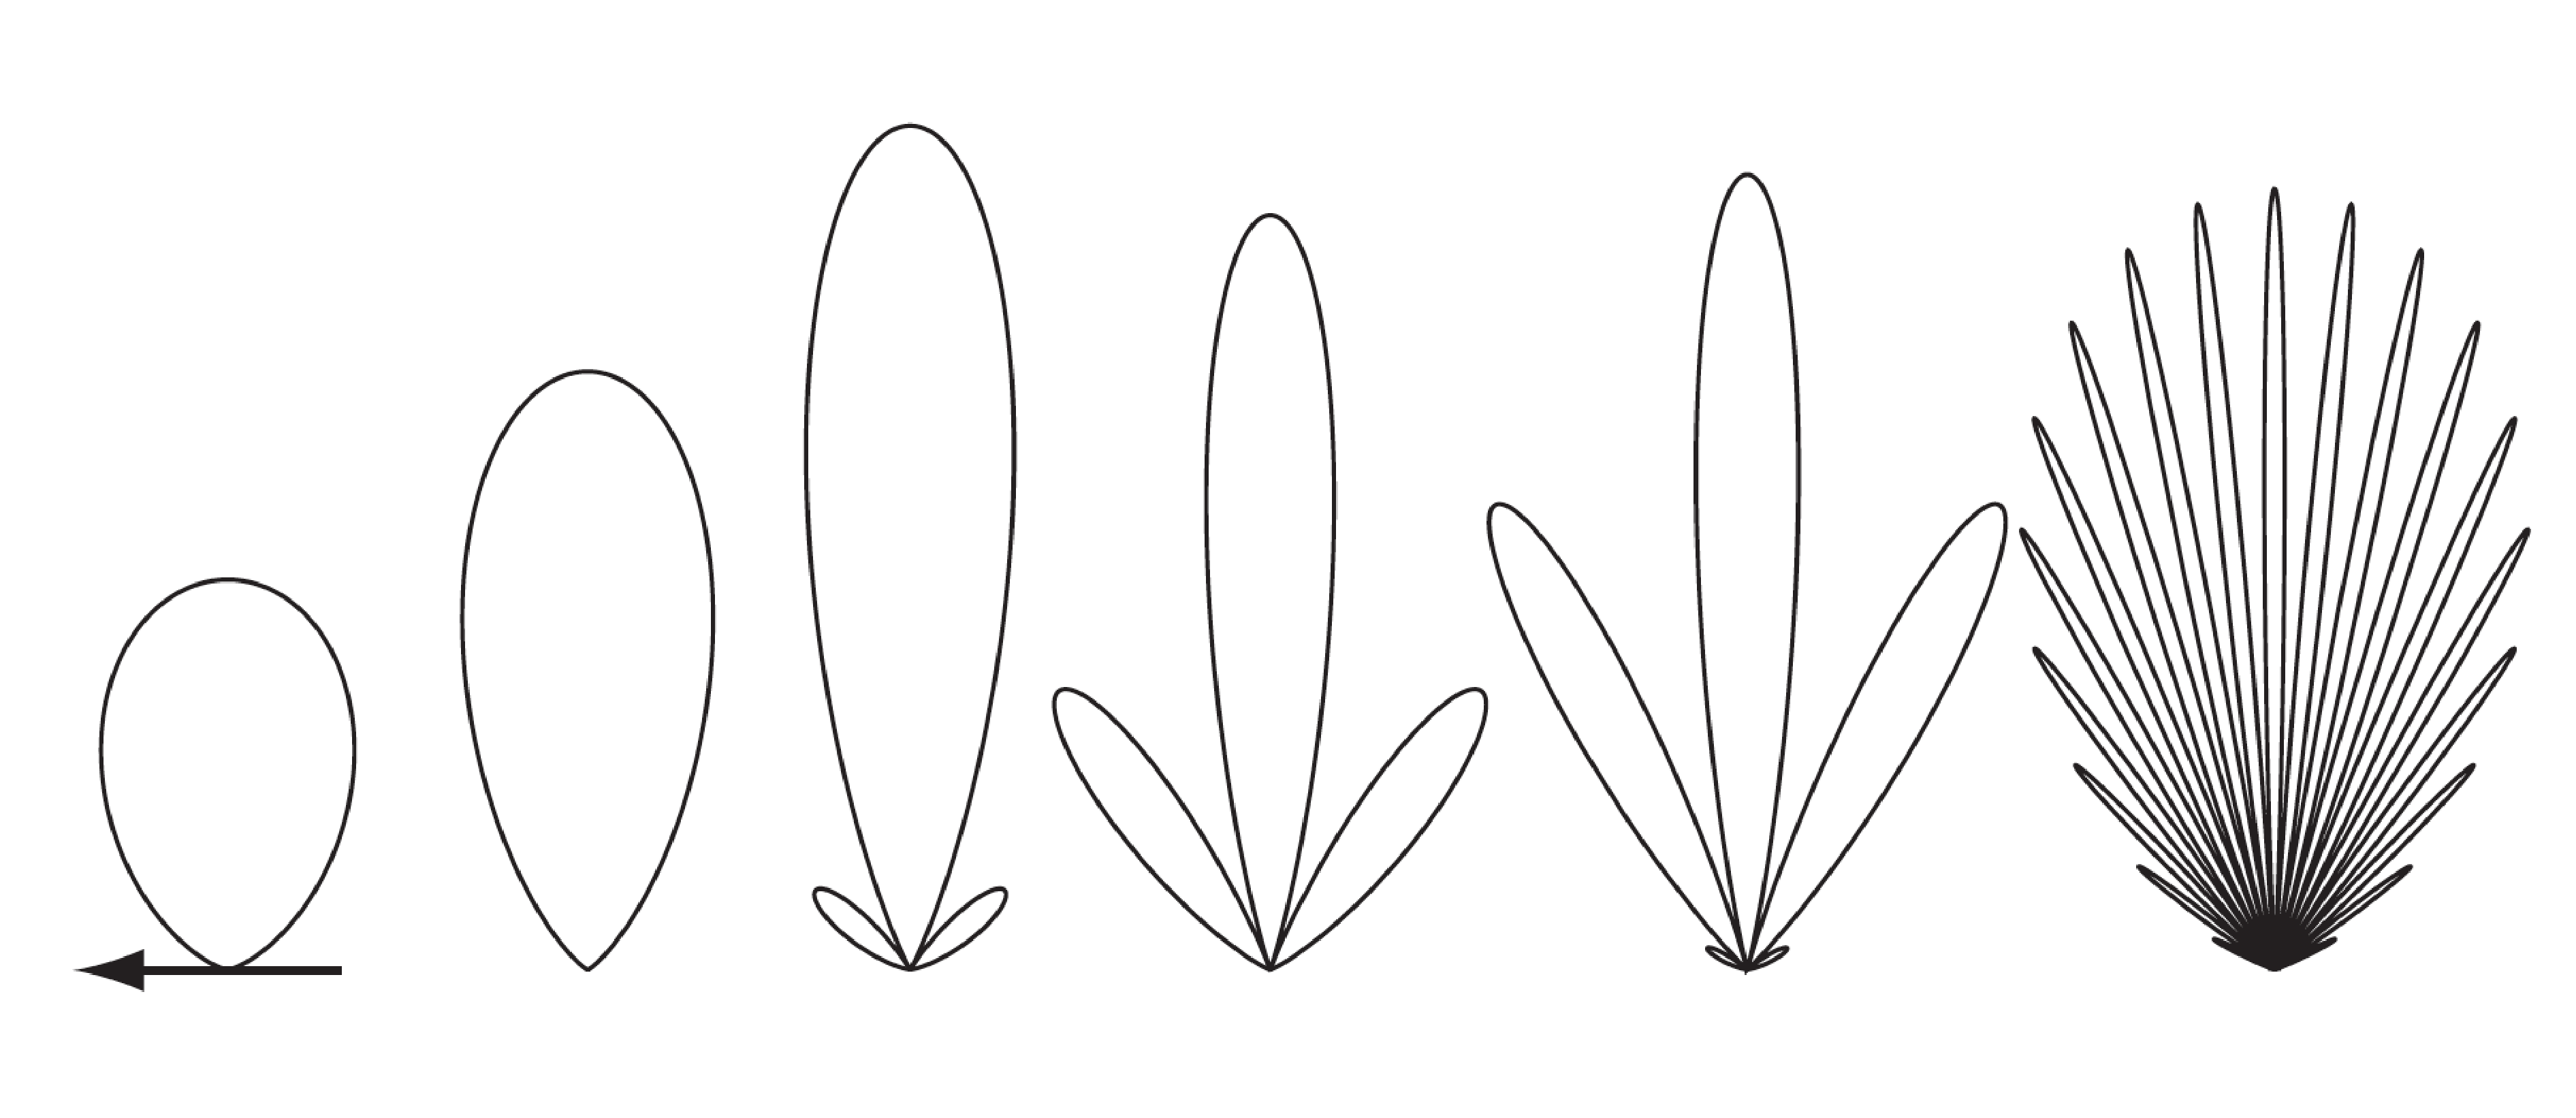
\includegraphics[width=0.8\textwidth]{two_atoms.pdf}
\end{center}
\caption[Radiation patterns for two dipoles]{Normalized radiation patterns $P(\theta;\ell)\sin\theta$ for the two dipoles for the distances between the dipoles $\ell=0,\,\pi,\,2\pi,3\,\pi,4\,\pi$, and $20\pi$ (left to right). These are a polar plots for $\theta\in[0,\pi]$,with the direction of the dipole and the $z$ axis denoted by the arrow in the $\ell=0$ graph.}
\label{TWOATOMS}
\end{figure}

As to the radiated power, the detuning from the resonance shifted by the cooperative-operative effects is the true gauge of resonance effects. We momentarily assume that this shift of reference point is implicit in the expression of the power in the two-atom radiation $P_2$, and simply replace $\Delta(\ell)\rightarrow\Delta$. On the other hand, if there were no cooperative-operative effects or interference between the radiations from the two dipoles, the total radiated power would simply be twice the radiated power from one dipole under the same driving field. The ratio of the actual two-atom power and the power from two independent dipoles
\beq
C = \frac{P_2}{2 P_1} = \frac{\gamma(\ell)[\Delta^2+\gamma^2]}{\gamma[\Delta^2+\gamma^2(\ell)]}
\eeq
is a reasonable measure of cooperativity, with $C=1$ applying to completely independent radiators.

The explicit expression follows immediately from Eq.~\eq{GAMMAL}. Because in the limit $\ell\rightarrow\infty$ we have $\gamma(\ell)\rightarrow\gamma$, we find $C\rightarrow1$ as expected. In the opposite limit $\ell\rightarrow0$ we have $\gamma(\ell)\rightarrow 2\gamma$, and the cooperative-operation of the dipoles depends in an essential manner on the detuning. If $|\Delta|\ll\gamma$, we have $C\simeq\half$. This means that on resonance the two atoms together radiate the same power as one single atom. On the other hand, with $|\Delta|\gg\gamma$, we have $C\simeq2$, and the two-atom sample radiates twice as much power as two independent atoms would. In fact, in this limit the radiated power can be expressed at all detunings as
\beq
P_2 = \frac{3 |E_0|^2}{2\{[\Delta/2\gamma]^2+1\}}\,,
\eeq
as if we had a single dipole with the dipole moment matrix element equal to $\sqrt2$ times the original dipole moment matrix element.

 Now, it is well known that on resonance the cross section for light scattering is independent of the dipole moment matrix element, so the cross section and scattered power are both independent of the dipole matrix element. On the other hand, far-off resonance the scattered power is in fact proportional to the square of the dipole matrix element times the linewidth, and as such is proportional to the fourth power of the matrix element. Hence, the power from two atoms should be four times the power from one atom, or twice the power from two independent atoms. The $\ell\rightarrow0$ limit is fully compatible with the observation that the two atoms have merged into one and the dipole matrix element has been multiplied by $\sqrt2$, with the proviso   that, as a result of atom-atom interactions, a shift of the resonance occurs that diverges in the limit $\ell\rightarrow0$.

There is an interesting little puzzle here: One would imagine that when one simply joins the two atoms, the dipole moment matrix element should be twice the matrix element for a single atom, not the multiple $\sqrt 2$. Granted, in quantum mechanics, when restricted to the state space of collective states that are invariant under the exchange of the two atoms, the factor in fact is $\sqrt2$. But here we have a completely {\em classical\/} situation. What gives?

To find the solution, let us momentarily take a variation of the classical Lorentz model for a dipole, namely two classical charged particles with charge $q$ and mass $m$ moving in the $z$ direction. Both particles are bound to their equilibrium positions with assumedly immovable neutralizing charges, so that there are restoring forces proportional to the square of the of natural frequency $\omega_0$ common to both of the oscillators. By a suitable choice of the origins of the coordinates, we make the equilibrium positions equal to zero. Nonetheless, we assume that in actuality the dipoles sit back to back as in the example of the present section, and much closer than the wavelength of the driving light from one another. The fields from one dipole, the moving charge and the stationary "nucleus", then add up to a force that attempts to move the other charge in the same $z$ direction. We characterize this force by the frequency $\Omega$. Finally, we assume that both of the dipoles are driven by the same external field $E$ at the frequency $\omega$. The equations of motion for the positive-frequency components of the positions of the two charges are then
\bea
\ddot{z}_1 = -\omega_0^2 z_1+ \Omega^2 z_2 + \frac{qE}{2m}e^{-i\omega t},\label{INDIVDIP1}\\
\ddot{z}_2 = -\omega_0^2 z_2+ \Omega^2 z_1 + \frac{qE}{2m}e^{-i\omega t}\,.
\eea
In terms of the normal modes
\beq
\eta_\pm = \frac{1}{\sqrt 2} (z_1 \pm z_2)
\eeq
the equations of motion read
\bea
\ddot{\eta}_+ &=& -(\omega_0^2-\Omega^2)\eta_+ +\frac{qE}{\sqrt2\, m} e^{-i\omega t},\label{COLLDIPP}\\
\ddot{\eta}_- &= &-(\omega_0^2+\Omega^2)\eta_-\,.
\eea
The resonance of the two modes $\eta_\pm$ are shifted in the opposite directions by the interaction between the dipoles. Besides, the ``nonradiating'' mode $\eta_-$ does not couple to the driving field at all. 

Let us now assume that there is some damping in the system that eventually leads to equilibrium, but which is otherwise negligible. For instance, assume that we drive the dipoles far-off resonance. Then no excitation of the mode $\eta_-$ is present. Moreover, a comparison of Eqs.~\eq{COLLDIPP} and~\eq{INDIVDIP1}  shows that for the same driving field strength $E$ and for the same detuning of the frequency $\omega$ from the respective resonance frequencies $\sqrt{\omega_0^2-\Omega^2}$ and  $\omega_0$, the steady-state oscillation amplitude of the collective mode $\eta_+$ would be a factor of $\sqrt 2$ larger that the amplitude of a single dipole.

This is ostensibly the $\sqrt 2$ for the collective response in quantum mechanics, but the normal modes are an auxiliary construct and as such have no a priori meaning in classical mechanics. We therefore consider the original displacement $z_1$ and $z_2$. These, in fact, oscillate in phase, and with the same amplitude as would one dipole for the same detuning from resonance. The total radiated electric field from the two dipoles will thus be twice the field from one dipole, and the radiated power is multiplied by four. Everything is as expected. The reason for the factor-of-two enhancement in radiated power is simply constructive interference of the two radiators. At least in the far-detuned case the quantum mechanical enhancement of the dipole moment matrix element by $\sqrt2$ is an illusion.


\section{Radiation power from Gaussian clouds of atoms}


\subsection{Continuous medium}

For the more general problem of $N$-atom gases, let us start with a hypothetical model with a continuous spatial distribution of atoms.

In terms of macroscopic electromagnetism, there is a monochromatic polarization of the sample
\beq
{\bf P}({\bf r},t) = \half\rho({\bf r}) \,{\bf d}({\bf r})e^{-i\omega t} + {\rm c.c.}\,,
\eeq 
where $\rho({\bf r})$ is the density of the sample  and $\bf d({\bf r})$ is the electric dipole of an atom at the position $\bf r$. Taking the atoms  to reside around the origin of the coordinates, in the far field with the distance $r\gg1$ and with $r$ much larger than the size of the sample, the terms  $\propto 1/R^2$ and $\propto 1/R^3$ in Eq.~\eq{dipolarE} are negligible and the  field  radiated by this polarization is
\bea
{\bf E}_R({\bf r})&\simeq&\frac{e^{ir}}{r} \int d^3r'\,e^{-i  \hat{\bf r}\cdot {\bf r}'}\rho({\bf r}')
\, [\hat{\bf r}\times{\bf d}({\bf r}')]\times\hat{\bf r}\,;
\label{SCATFIELD}
\eea
$\hat{\bf r}={\bf r}/r$ is the unit vector that points from the source at $\simeq 0$ to the field point. 

For easy analysis, we model the density with a Gaussian,
\beq
\rho({\bf r}) = \frac{3\sqrt3N}{2\sqrt2\pi^{3/2} R^3}\, e^{-\frac{3r^2}{2R^2}}\,,
\label{CONT_DEN}
\eeq
where $N$ is the atom number and $R$ is the size scale of the sample. The parametrization is chosen in such a way that the rms value of $|\br|$ equals $R$. In the limit $R\gg1$ there will be a narrow cone of radiation around the direction of the incoming beam; let us denote the angle from the incident beam by $\theta$.  

For a tangible example, let us take a $\sigma_+$ circularly polarized plane wave propagating in the $z$ direction, writing
\beq
\bE_0(\br) = E_0\, e^{iz}\,\hat{\bf e}_+;\quad \hat{\bf e}_+=-\frac{1}{\sqrt{2}}(\hat{\bf e}_x + i \hat{\bf e}_y)\,.
\label{incomingE}
\eeq
The key assumption here is that the incoming light dominates even inside the sample. Accordingly, we write the dipole moment of an atom at $\br$ simply as
\bea
{\bf d}({\bf r})=\alpha\bE_0(\br)=\alpha E_0\, e^{iz}\,\hat{\bf e}_+.
\eea

Now we turn back to the radiated field:
\bea
{\bf E}_R({\bf r})&=&\frac{e^{ir}}{r}\int d^3r^{\prime} e^{-i\hat {{\bf n}} \cdot {\bf r}^{\prime}} \rho({\bf r^\prime}) [ \hat { \bf n} \times  {\bf d}({\bf r}^{\prime}) ]  \times \hat {\bf n}\nonumber\\
&=&\frac{3\sqrt{3}\alpha NE_0e^{ir}[ (\hat { \bf n} \times \hat{{\bf e}}_+)  \times \hat {\bf n}]}{2\sqrt{2}\pi ^{3/2}R^3r}\int d^3r^{\prime} e^{-i\hat {{\bf n}} \cdot {\bf r}^{\prime}}e^{iz}e^{\frac{-3r^{\prime2}}{2R^2}}\nonumber\\
&=&\frac{\alpha NE_0e^{ir-\frac{1}{3}R^2(1-\cos \theta)}}{r}[ (\hat { \bf n} \times \hat{{\bf e}}_+)  \times \hat {\bf n}].
\eea
The magnitude of the Poynting vector is 
\bea
S_R({\bf r})&=&\frac{|{\bf E}_R|^2}{8\pi}=\frac{\left|\alpha\right|^2N^2 E_0^2 e^{-\frac{2}{3}R^2(1-\cos \theta)}|(\hat { \bf n} \times \hat{\bf e}_+) \times \hat {\bf n} |^2}{8 \pi r^2} \nonumber\\
&=&\frac{\left|\alpha\right|^2N^2 E_0^2 e^{-\frac{2}{3}R^2(1-\cos \theta)} (1+\cos^2 \theta)}{16 \pi r^2}.  
\eea
The total power of the radiation is readily obtained as
\bea
P_R&=&\int r^2 S_C({\bf r})\,d^2\Omega\nonumber\\
&=&\frac{3\left|\alpha\right|^2N^2E_0^2\left[(4R^4-6R^2+9)-e^{-\frac{4R^2}{3}}(4R^4+6R^2+9)\right]}{32R^6}.
\eea
Here the intensity of the scattered light scales with the square of the atom number, $N^2$. This is similar to an important characteristic of superradiance. However, it is still early for conclusions. Let us first inspect a more realistic problem, where we have discrete atoms instead of an oversimplified continuous medium.

\subsection{Independent discrete radiators}
Take a a collection of $N$ identical dipoles sitting at the positions ${\bf r}_i$ in the incoming field, and assume that each of these dipoles radiates a field ${\bf E}_i({\bf r})$ {\em independently}. In other words, we assume that only the incoming field $\bE_0$ drives each dipole. The total dipolar field at the point ${\bf r}$ is then
\beq
{\bf E}_D({\bf r}) = \sum_i {\bf E}_i({\bf r})\,,
\eeq
with
\beq
{\bf E}_i({\bf r}) = \alpha{\cal E}(\br,\br_i)\cdot\bE_0(\br_i)\,.
\eeq
Suppose we are in the far field where the Poynting vector is obviously radial and its absolute value is related in the same simple way to the square of the electric field as for a single dipole. The  absolute value is
\bea
S_R(\br) &=& \frac{1}{8\pi} \bE_D(\br)\cdot\bE_D^*(\br )\nonumber\\
&=& \frac{1}{8\pi} \sum_{i,j} \bE_i(\br)\cdot\bE_j ^*(\br)\,.
\eea

In fact, it may be that the atoms reside in some fixed configuration, but for a gaseous sample it is more physical to take their position to be randomly distributed in space. We take the position of each atom to be a random variable independent of the positions of the other atoms, governed by same probability density function $f(\br)$. Then for a given $\br$, $\left\{\bE_1(\br),\cdots,\bE_i(\br),\cdots \bE_N(\br)\right\}$ is a set of independent and identically distributed random variables. Therefore, the average outward energy flux (over many samples of the gas) is determined from
\bea
8 \pi\bar{S}_R &=&\left\langle
 \sum_{i\ne j} \bE_i(\br)\cdot\bE_j^*(\br)+\sum_i \bE_i(\br)\cdot\bE_i^*(\br)
\right\rangle\nonumber\\
&=&
 \sum_{i\ne j} \left\langle\bE_i(\br)\right\rangle
\cdot\left\langle\bE_j^*(\br)\right\rangle +
\sum_{i} \left\langle\bE_i(\br)\cdot\bE^*_i(\br)\right\rangle\nonumber\\
&=&N(N-1)|\left\langle \bE_i(\br)\right\rangle|^2 + N \left\langle\bE_i(\br)\cdot\bE^*_i(\br)\right\rangle\,.
\eea
The first term represents coherent scattering, as if the atom was spread out to a continuous dielectric material with the spatial shape specified by $f(\br)$. It arises from adding the fields of different radiators, and is essentially proportional to $N^2$. The second term $\propto N$ is for incoherent scattering, or the sum of intensities radiated by the individual atom. It is present because the gas is not a continuous dielectric medium, but consists of discrete scatterers.

Incidentally, while this argument may not be as widely known as it deserves, it is far from novel: Einstein used analogous reasoning to demonstrate the atomic (molecular) nature of matter when it was still under doubt~\cite{ANDP:ANDP200590026}. The blue sky comes from incoherent scattering. If air were a continuous dielectric medium, it would not scatter sunlight sideways and the sky would be black.

For comparison, we apply the same incoming light as in Eq.~\eq{incomingE} and the position distribution for the atoms is still taken to be Gaussian,
\beq
f(\br) = \frac{3\sqrt3}{2\sqrt2\,\pi^{3/2}R^3}\,e^{-\scriptstyle\frac{3r^2}{2R^2}}\,.
\eeq
Given the usual polarizability $\alpha$, the far field (the $1/r$ part of dipole radiation) averaged over the positions of an atom, the absolute square of the former, and the  absolute square  of the field averaged over the positions give
\bea
\langle \bE_i(\br)\rangle &=& \alpha E_0 e^{ir-\hbox{$\frac{1}{3}$}R^2(1-\cos\theta)}[(\hat{\bf r}\times\hat{\bf e}_+)\times\hat{\bf r}]\,\frac{e^{ir}}{r},\\
|\langle \bE_i(\br)\rangle|^2 &=& \frac{|\alpha |^2| E_0|^2[3+\cos (2 \theta )] e^{\frac{2}{3} R^2 [\cos (\theta
   )-1]}}{4 r^2},\\
   \langle |\bE_i(\br)|^2\rangle &=& \frac{|\alpha |^2| E_0|^2[3+\cos (2 \theta )]}{4 r^2}\,.
\eea
The total radiated power becomes
\bea
P_S&=&\frac{|\alpha|^2 |E_0|^2}{3}\Bigg\{
N(N-1)\frac{9\left[(4R^4-6R^2+9)-e^{-\frac{4R^2}{3}}(4R^4+6R^2+9)\right]}{32R^6}\nonumber\\
&&+N\Bigg\}\,.
\label{PN}
\eea

\begin{figure}[h!]
\begin{center}
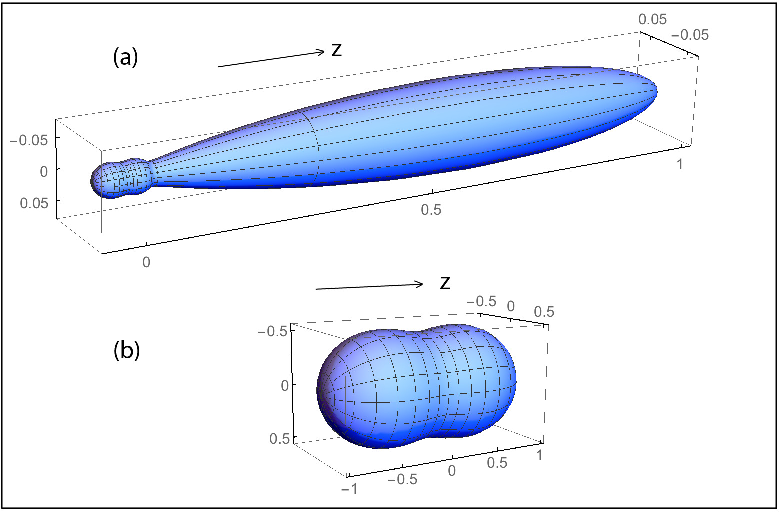
\includegraphics[width=\textwidth]{angular.pdf}
\end{center}
%\caption{Log-log plot of the total radiated power vs. the number of atoms from two types of models. $R$=1 and $\delta=600$ in both cases. The solid line is the result of Eq.~\eq{PN}. Ret dots denote the results from simulations.}
\caption{Normalized radiation patterns $P_N(\theta,R)\sin\theta$ for two Gaussian samples with $R=10$ in (a) and $R=0.1$ in (b). For both cases, the number of atoms is $N=20$, and the detuning is $\delta=600$.}
\label{ANGULAR}
\end{figure}

The main utility of these formulae is that they will serve as references with which to compare numerical results. A few incidental results could be noted, however.  The part $\propto N(N-1)$ in Eq.~\eq{PN} is the same as it would be for the continuous atom density in Eq.~\eq{CONT_DEN}, except for the factor of $N(N-1)$ instead of $N^2$. The intensity of the radiation in the forward direction, at $\theta=0$, coherent and incoherent components, add up to exactly $N^2$ times the intensity from a single atom. The bigger the sample, the narrower the cone in the direction $\theta=0$ for coherent scattering.  This aspect is demonstrated in Fig.~\ref{ANGULAR}. The sample acts as an antenna that directs the radiation in the forward direction. Nevertheless, the total power decreases with increasing size of the cloud.

Conversely, in the limit $R\rightarrow0$ the intensity in all directions is enhanced by a factor $N^2$, and of course so is the total power. Given the Dicke cooperative regime as discussed in Sec.~\ref{DICKESTORY}, a reader might erroneously interpret such an enhancement as a cooperative phenomenon. This cannot be, because in this example we have simply added the fields from independent radiators.

%Last but not least, the difference between the continuous medium model and the independent radiators model in the total scattering power is given by
%\bea
%P_N-P_C&=&\frac{N\left|\alpha\right|^2E_0^2}{3}\nonumber\\
%&&\cdot\left\{1-\frac{9\left[(4R^4-6R^2+9)-e^{-\frac{4R^2}{3}}(4R^4+6R^2+9)\right]}{32R^6}\right\}
%\label{diffNandC}
%\eea

\subsection{Simulation of the power in scattered light} 

When the dipolar fields from all the other radiators are taken into account, an analytical calculation for the total power is impractical and we have to utilize simulations. 

\begin{figure}[h!]
\begin{center}
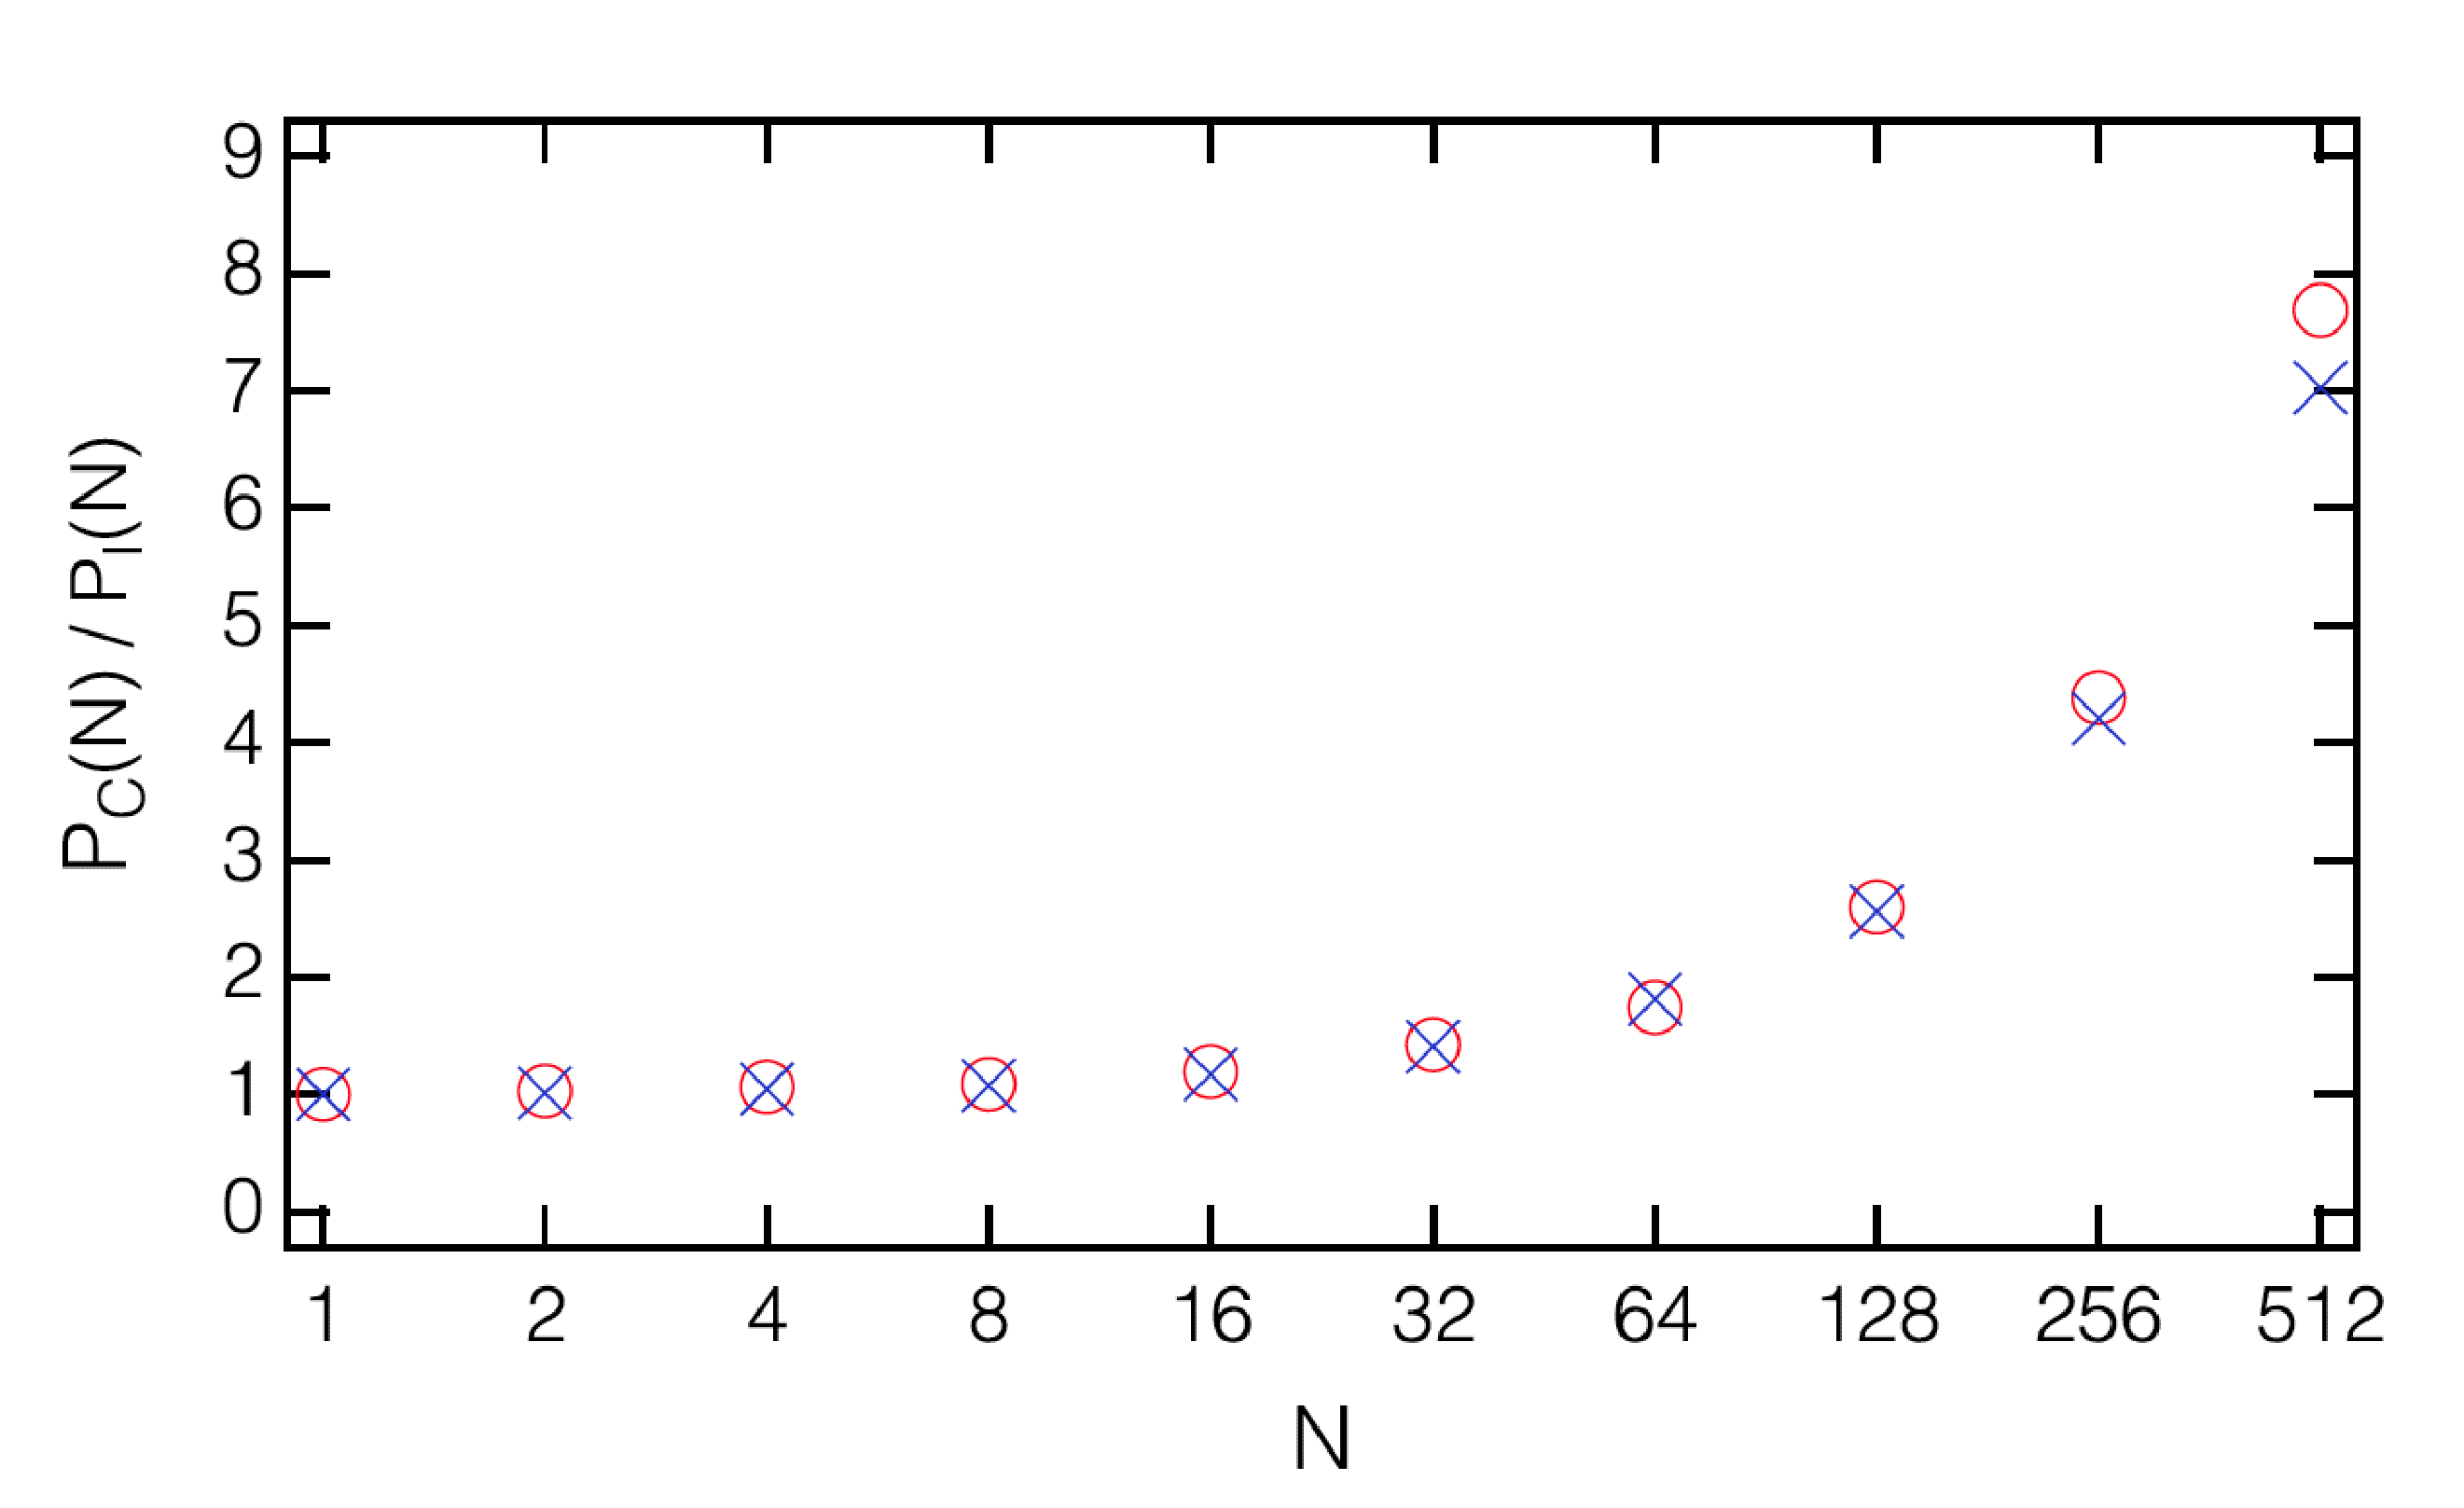
\includegraphics[width=\textwidth]{Pc_Pi.pdf}
\end{center}
%\caption{Log-log plot of the total radiated power vs. the number of atoms from two types of models. $R$=1 and $\delta=600$ in both cases. The solid line is the result of Eq.~\eq{PN}. Ret dots denote the results from simulations.}
\caption{Ratio of the numerically simulated scattered light power to the power from independently radiating atoms plotted for varying atom number $N$ for a Gaussian cloud with the rms radius $R$ satisfying $R=10$. The detuning is varied in such a way that the estimated optical thickness through the center of the cloud is $10^{-2}$ for all $N$. The circles and crosses are for different signs of the detuning, so that the cloud acts as either a focusing or a defocusing lens.}
\label{PCANDPN}
\end{figure}



We plot in Fig.~\ref{PCANDPN} the ratio of the numerically simulated collective power to the independent-atom power, $P_C(N)/P_I(N)$, for different numbers of the atoms $N$. Here the cloud radius is $R=10$. All of the data points are averaged over a large number of random positions of the atoms. While we vary the atom number and hence the density, we also vary the detuning in such a way that the estimated optical thickness for a ray of light going straight through the center of the cloud would be $10^{-2}$ so that absorption of light and indeed scattered dipole radiation should not be major factors. We have both positive (circles) and negative (crosses) detunings that make the gas either a focusing or defocusing lens.

The surprise here is that by $N=128$ when the collectively scattered power already more than doubles the independent-atom power, the central density is only $\rho=0.03$. We think that cooperative-operation sets in much earlier than expected, namely, around $\rho=1$, and we suspect that the same applies elsewhere too.


%The solid line in Fig.~\eq{PCANDPN} reflects the analytical result of a Gaussian cloud of independent radiators as given by Eq.~\eq{PN} and the red scatters represents the results of  radiators with dipole-dipole interactions.  
 
%We notice that the total power with cooperativity exceeds at small atom numbers but the situation reverses at large $N$, where the gas radiates much less then one would expect according to Eq.~\eq{PN}. This is a clear signature of cooperativity (for the only difference in this two models is the presence of light rescattering between atoms. ?)

\section{Shifts of resonance line in a circular disk}

Aside from total radiated power, spectroscopic evidence of cooperativity is also of interest to us. To study it, we replace the Gaussian cloud with a gas sample uniformly distributed inside a circular-disk shape container. This geometry has been addressed recently both in experiments and in theory~\cite{PhysRevLett.108.173601,Javanainen:16}.

The focus here is on the Lorentz-Lorenz (LL) shift and on the collective Lamb shift (CLS). 
We have summarized in Chapter 3 the argument from Ref.~\cite{FRIEDBERG1973101} that for a slab configuration, a uniform-density medium restricted to the interval $z\in [0,h]$, and for a plane wave with the wave number $k=\omega/c$ propagating in the $z$ direction, the absorption line should be shifted by
\bea
\Delta_L=\Delta_{LL}-\frac{3}{4}\Delta_{LL}\left(1-\frac{\sin 2hk}{2hk}\right);\,\quad\Delta_{LL}=-\frac{\rho\mathcal{D}^2}{3\epsilon_0\hbar} = -2\pi\rho k^{-3}\gamma
\label{LL_CLS}
\eea
from the atomic resonance. Here $\Delta_{LL}$, a redshift, is the standard LL shift, and $\Delta_L$ is the CLS as in Ref.~\cite{FRIEDBERG1973101}.  This is also the CLS verified in the experiments~\cite{PhysRevLett.108.173601}, albeit using hot atomic samples with moving atoms. As is obvious from Eq.~\eq{LL_CLS}, for the time being we have reverted to the standard SI units.

The original derivation of the CLS in Ref.~\cite{FRIEDBERG1973101}  was an elaborate QED argument. However, we now know~\cite{PhysRevLett.108.173601,Javanainen:16} that the same result can be obtained from the standard electrodynamics of polarizable media. The local-field corrections giving the $LL$ shift are inserted by hand as usual, while the oscillatory part $\propto\frac{3}{4}$ comes from etalon effects, reflections of light from the front and back surfaces of the slab. According to this argument, the LL shift should be there regardless, whereas the oscillatory part is valid in the limit of low atom density only.

In the face of the multitude of remarks pulling in different directions, it is of great interest to find out what the {\em exact\/} solution to the light propagation problem would say. That is why we solve the light propagation problem using stochastic classical-electrodynamics simulations~\cite{PhysRevA.59.649,PhysRevE.69.026605,PhysRevLett.101.103602,1367-2630-14-5-055001,PhysRevA.86.031602,PhysRevB.86.085116,PhysRevB.86.205128,PhysRevA.88.033844}. As discussed before, in the simulations we start with $N$ atoms fixed at positions $\br_i,\, i=1,\dots,N$, each with an assumedly isotropic polarizability $\alpha$, and form the closed set of linear equations~\eq{FEQ}. Having solved these equations numerically, at least in principle we have the electric field amplitude everywhere as in Eq.~\eq{EF}. This computation is done for a number of random positions of the atoms compatible with the geometry of the sample, and the results are averaged.

Of course a truly exact numerical solution for an infinite slab is impossible, as it would require infinitely many atoms. In the simulations reported in the present chapter we use a circular disk with the radius $R=\sqrt{256/\pi}k^{-1}$, so the area is $A=256k^{-2}$. We vary the thickness of the disk $h$ but keep the density $\rho=N/hA=2k^3$ constant in the examples of the present chapter, so that the number of atoms $N$ varies accordingly. A circularly polarized plane wave comes in perpendicular to the face of the disk. Analogous numerical experiments, although for different purposes, have been described in Refs.~\cite{1367-2630-14-5-055001,PhysRevA.86.031602}.  

A serious complication follows from the use of the finite-size disk, namely, diffraction. Extinction of light upon propagation through a sample means that the incoming and the reradiated light interfere destructively. A finite-size disk does not radiate a plane wave, so we lose what is known as mode matching between the radiation from the dipoles and the incoming plane wave. In fact, an exact computation of the transmitted light does not reproduce satisfactorily even the most rudimentary results of the optics of an infinite slab.

To circumvent this problem we resort to the method introduced in Ref.~\cite{1367-2630-14-5-055001}. Basically, we obtain the dipole moments of the atoms in the sample, but when calculating the field transmitted through the sample, we assume that each dipole radiates a plane wave that is automatically mode matched with the incoming wave. As before, let us assume that the incoming plane wave propagates in the $z$ direction. For a disk of radius $R$, the amplitude of the assumed plane wave from a dipole at ${\bf r}_j$ is computed as
\beq
\bE_j({\bf r}) = \frac{ik}{2\pi\epsilon_0 R^2} [\bd({\bf r}_j)-\hat{\bf e}_z \cdot\bd({\bf r}_j)\,\hat{\bf e}_z] e^{ik(z-z_j)}\,.
\label{TRLIGHT}
\eeq
This method produces good results even for a disk as small as the one we use in our simulations. In the limit of a dilute sample when we expect classical optics to apply, we get to within a few percent of the predictions of classical optics for an infinite slab.

We generate a number of random samples, from 64 to millions, of atomic positions evenly distributed inside the disk, compute the transmitted light as a function of the detuning $\Delta$ for each sample, and average the results. We report the optical thickness $D$ defined in terms of power transmission coefficient $T$ as $D=-\ln T$. The advantage here is that in a medium that obeys Beer's law the optical thickness would be linearly proportional to the thickness $h$, but would otherwise have the same line shape $D(\Delta)$ for all thicknesses. The scale of computations can be large; a publication-scale project can take $10^5$ hours of CPU time. The production runs we are discussing in the present chapter were mostly done on what is functionally a very large computer cluster, the Open Science Grid~\cite{OSG}.

Figure~\ref{HOMO_D} shows the optical thickness $D$ as a function of detuning $\Delta$ for the sample thicknesses $hk=0.25, 0.5, 1.0$ and $2.0$, with the corresponding atom numbers $N=128, 256, 512,$ and $1024$. For comparison we also give the predicted LL shift of this atom density as a dashed vertical line. The absorption lines are not Lorentzian. While the line broadens with increasing atom number and may be noticeably asymmetric, the maximum nevertheless moves very little. The shift, if any, is at most a few percent of the LL shift. No manifest LL shift is present, nor a CLS. Given that the LL shift comes from a universally accepted and widely used local-field arguments, its absence in the simulations is quite remarkable.


\begin{figure}[h!]
\begin{center}
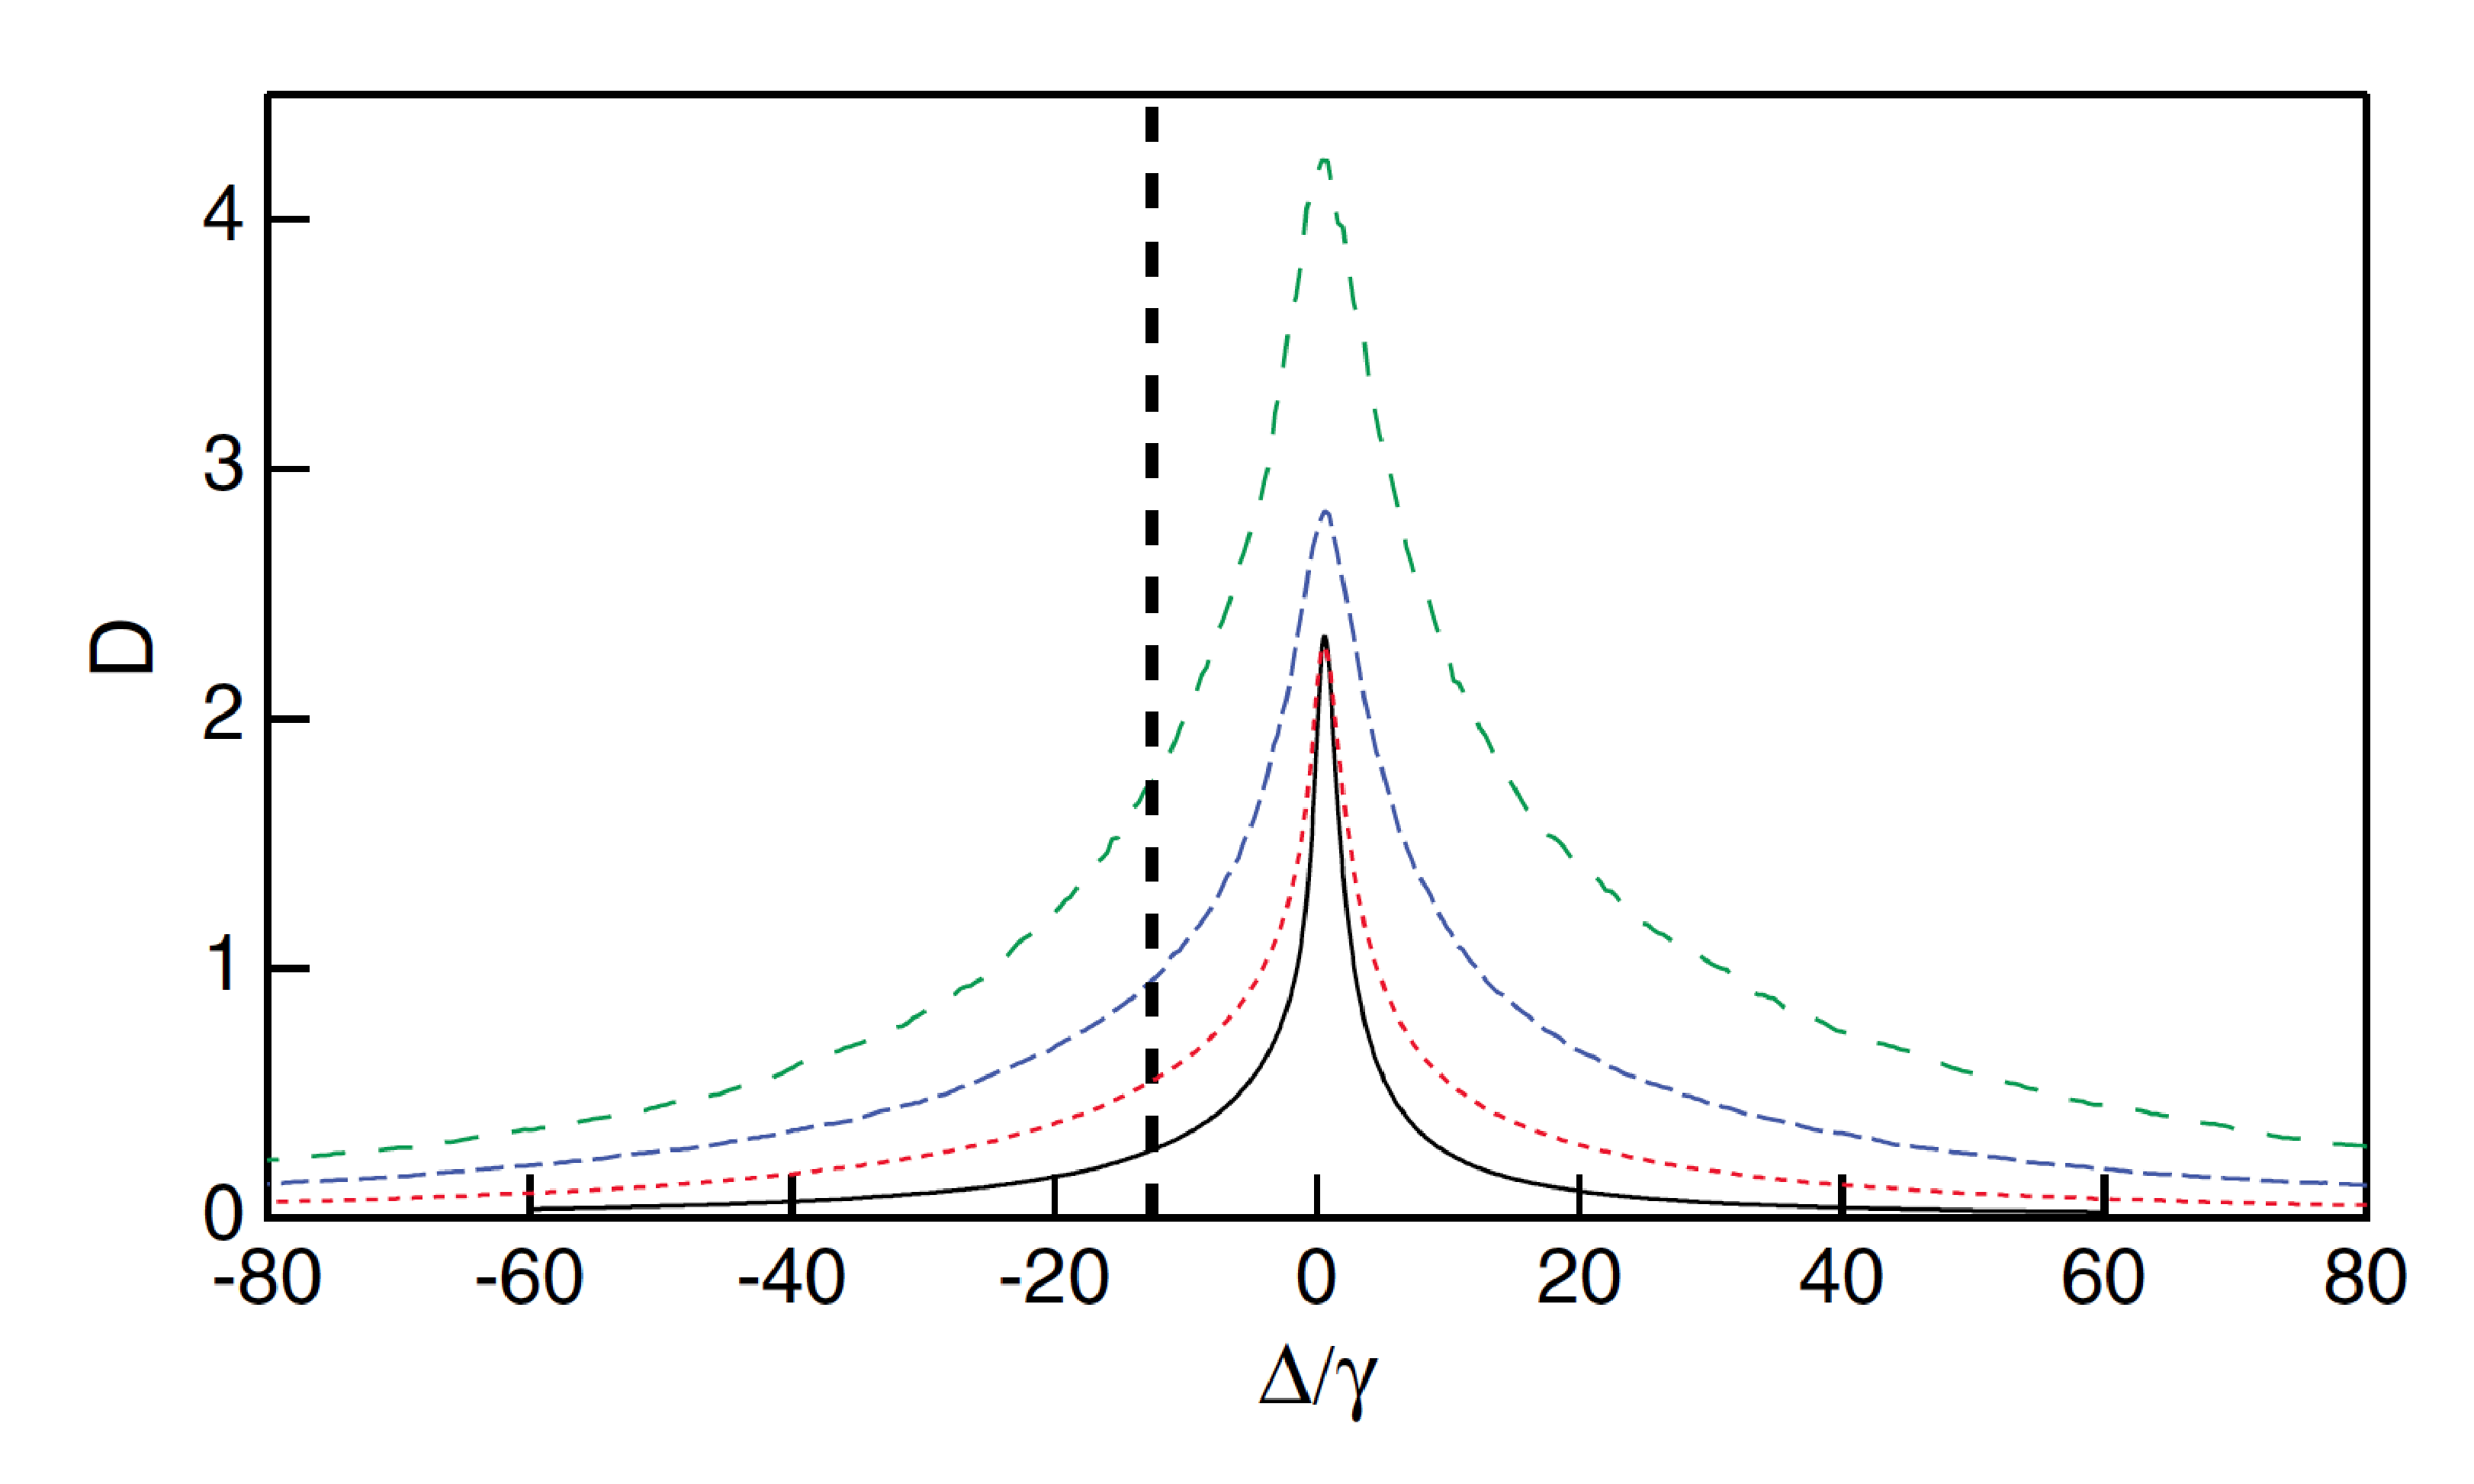
\includegraphics[width=\textwidth]{homo_D.pdf}
\end{center}
\caption{Optical depth $D$ versus detuning $\Delta$ for stationary atoms for sample thicknesses $hk=0.25, 0.5, 1.0$, and $2.0$, from bottom to top; the corresponding atom numbers are $N=128, 256, 512,$ and $1024$. The dashed vertical line shows where the center of the line would be if the naive Lorentz-Lorenz shift applied.}
\label{HOMO_D}
\end{figure}

Before introducing new factors into our simulations such as the actual motion of the atoms, we repeat the numerical experiments with stationary atoms in the circular disk. However, this time we assume that the resonance frequency of each atom is also shifted by a Gaussian random variable with zero mean and the rms value $\omega_D=100\gamma$. This is a basic model for the Doppler shifts that follow from the motion of the atoms. Given that we have a different resonance frequency for each atom, the atomic sample is termed ``inhomogeneously broadened''. In contrast, if the atoms are stationary or move so slowly that there is no significant effect on spectroscopy, as in our simulations until now, the sample is called ``homogeneously broadened''.

An example spectrum is shown in Fig.~\ref{INHOMO_D}. The line shape has an appearance common in the spectroscopy of inhomogeneously broadened samples. Accordingly, we fit it with the Voigt profile $V(\Delta-s;\Gamma,\Omega_D)$, convolution of a Lorentzian with the HWHM $\Gamma$ and a Gaussian with the rms width $\Omega_D$. We are particularly interested in the shift $s$ of the spectrum from the atomic resonance.

\begin{figure}[h!]
\begin{center}
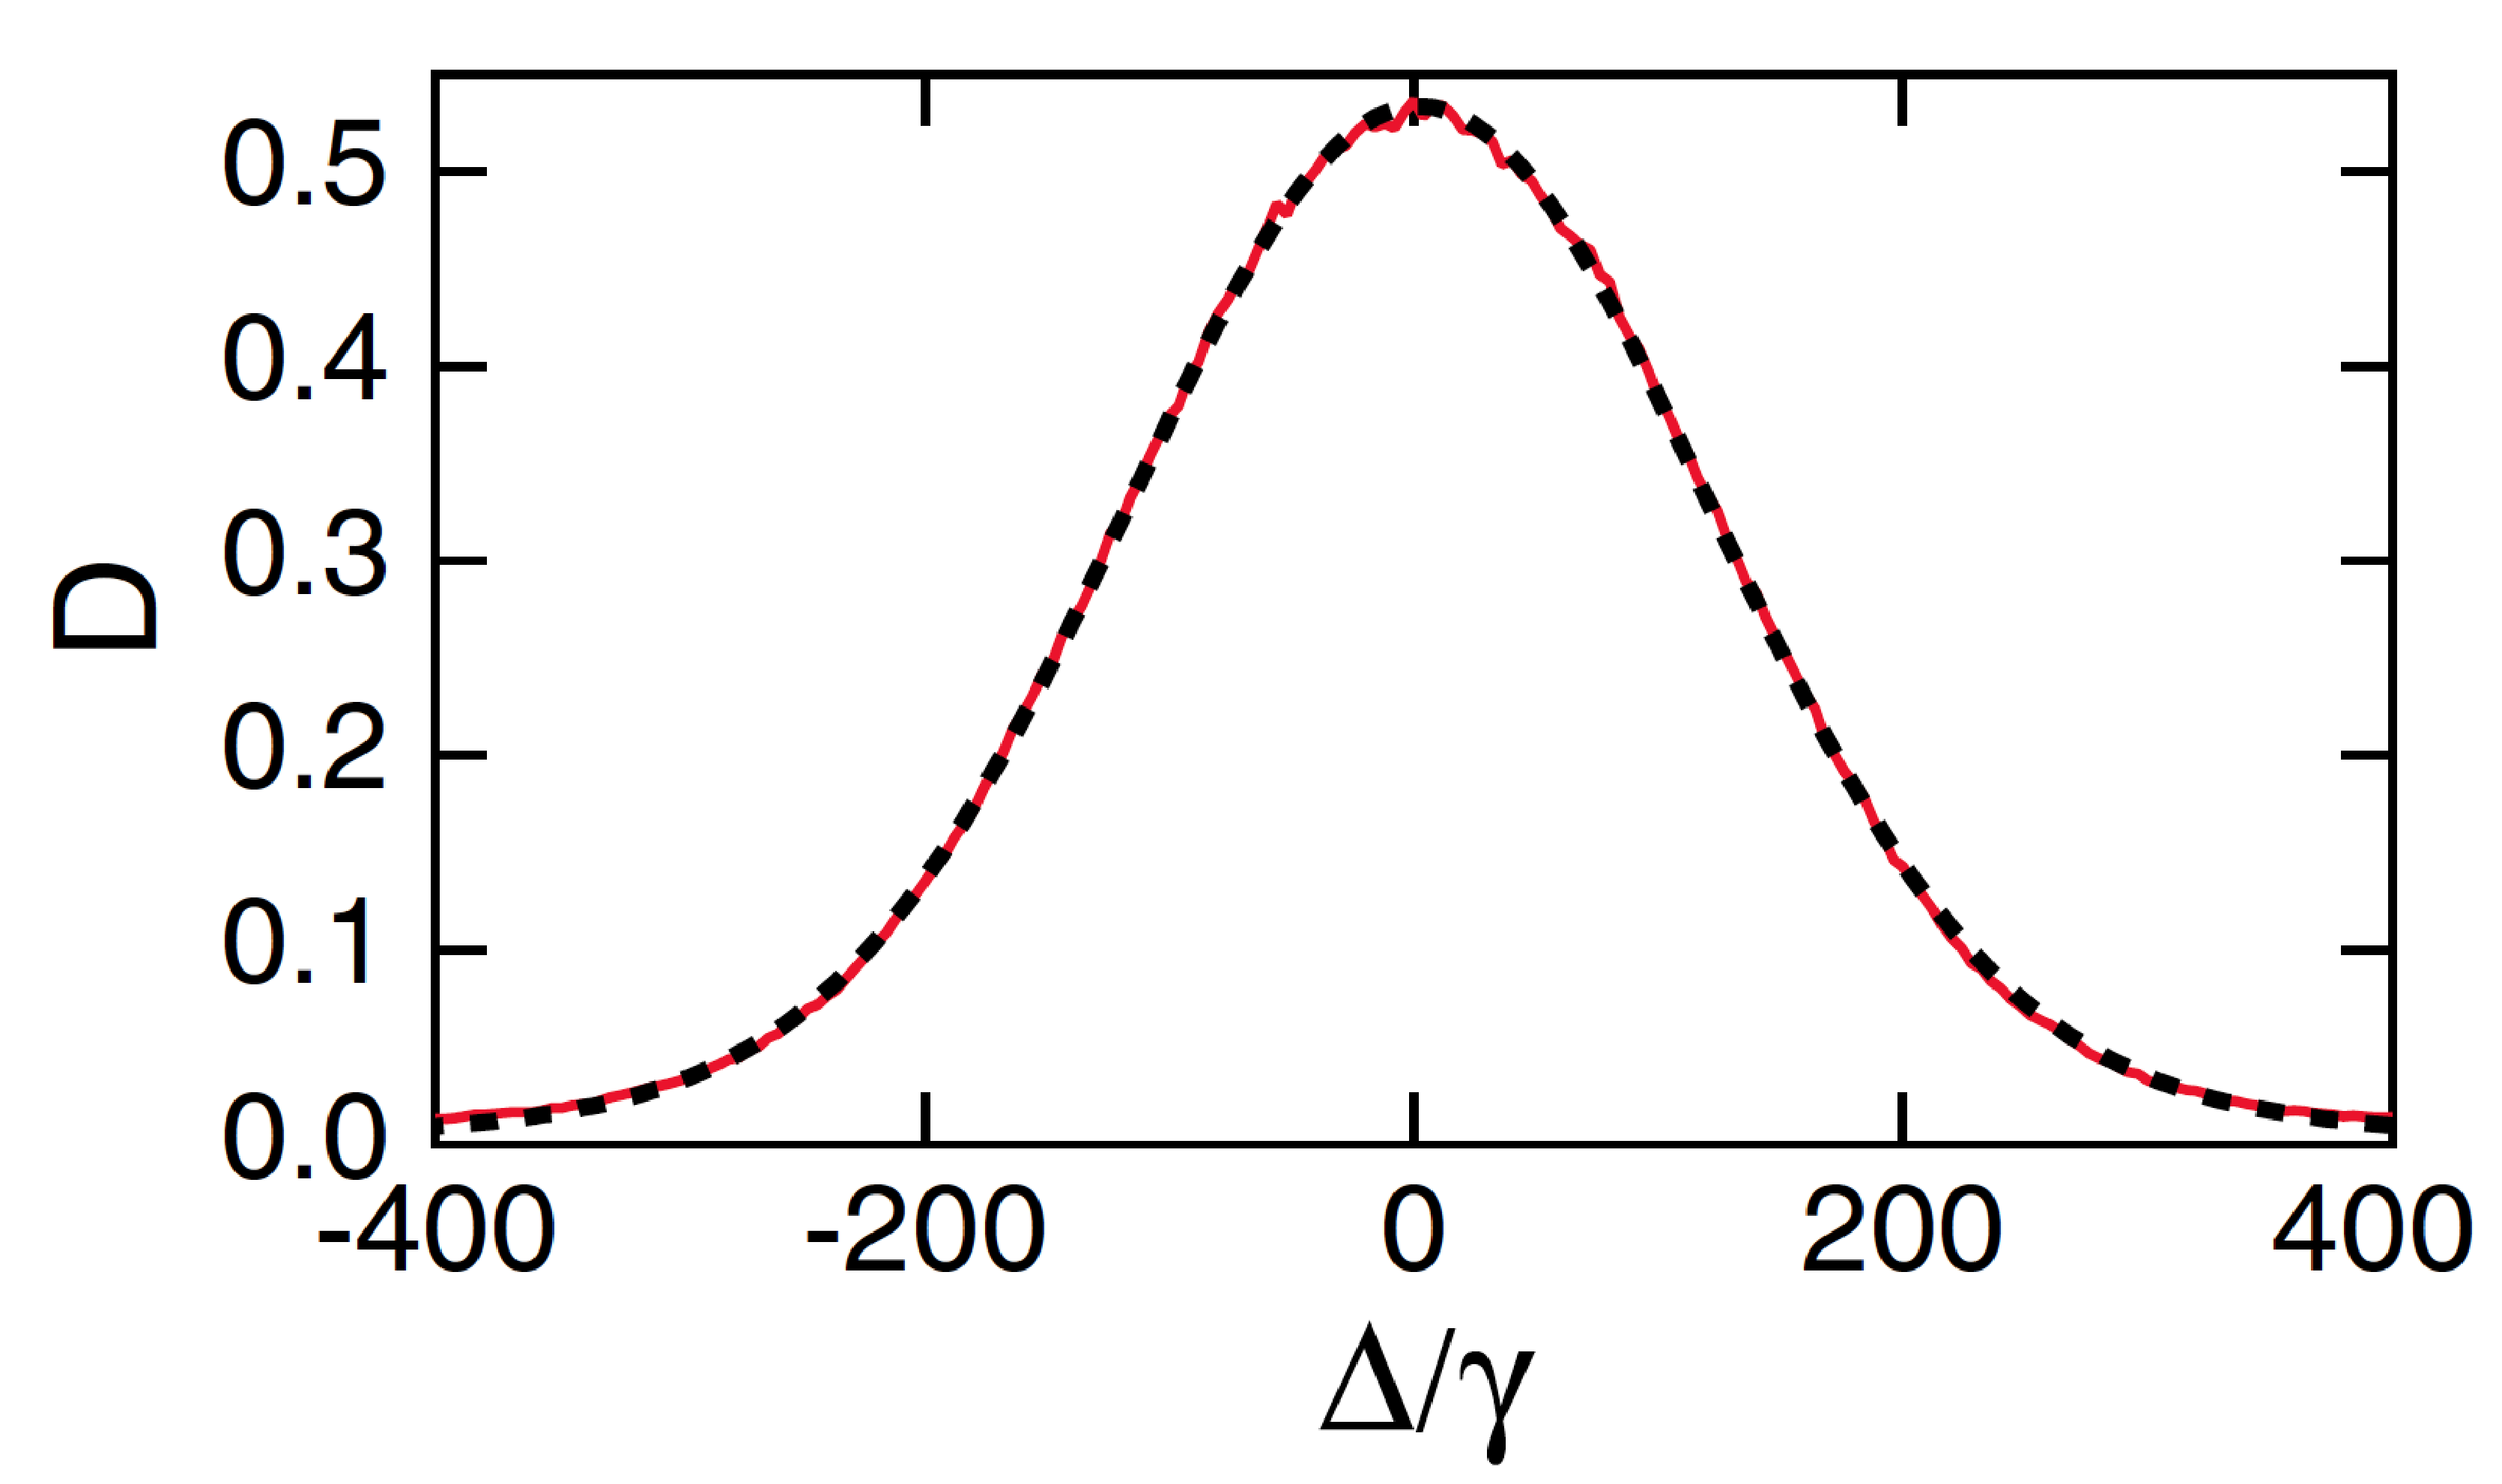
\includegraphics[width=\textwidth]{inhomo_D.pdf}
\end{center}
\caption{Optical depth of the sample $D$ with thickness $hk=1.5$, and, hence, $N=768$ atoms, as a function of the detuning for a sample with the inhomogeneous linewidth $\omega_D=100\gamma$. This numerical experiment (solid red line) is an average of 1024 samples, the fit with a Voigt profile (dashed black line) has the parameters $s=2.15\gamma$, $\Gamma=17.74\gamma$, and $\Omega_D=112.83\gamma$.}
\label{INHOMO_D}
\end{figure}

We plot the shift of the resonance $s$ for inhomogeneously broadened samples as a function of the thickness of the disk $h$ in Fig.~\ref{STATIC_CLS} as filled circles.  In these fits the widths of the Lorentzian and Gaussian components of the Voigt profile $\Gamma$ and $\Omega_D$ were also allowed to vary, and of course there was an overall multiplicative factor to fit.

The shift tends to zero at small thicknesses. In this limit the physics clearly becomes two dimensional, for a fixed three-dimensional density the relevant two-dimensional area density tends to zero, and eventually the atoms must radiate completely independently. 

We also plot the CLS, Eq.~\eq{LL_CLS}, as a solid line. Numerical data and theory show similar oscillations, albeit differing approximately by an additive constant. In Fig.~\eq{STATIC_CLS} we also plot as a dashed line the vertically translated version of the theory to fit the numerical data points with $hk\geq 1$. An additive term was also fitted to the experiments~\cite{PhysRevLett.108.173601} before they gave agreement with Eq.~\eq{LL_CLS}. The agreement of our numerical experiments with the CLS theory is on a similar footing as in the real experiments.


\begin{figure}[h!]
\begin{center}
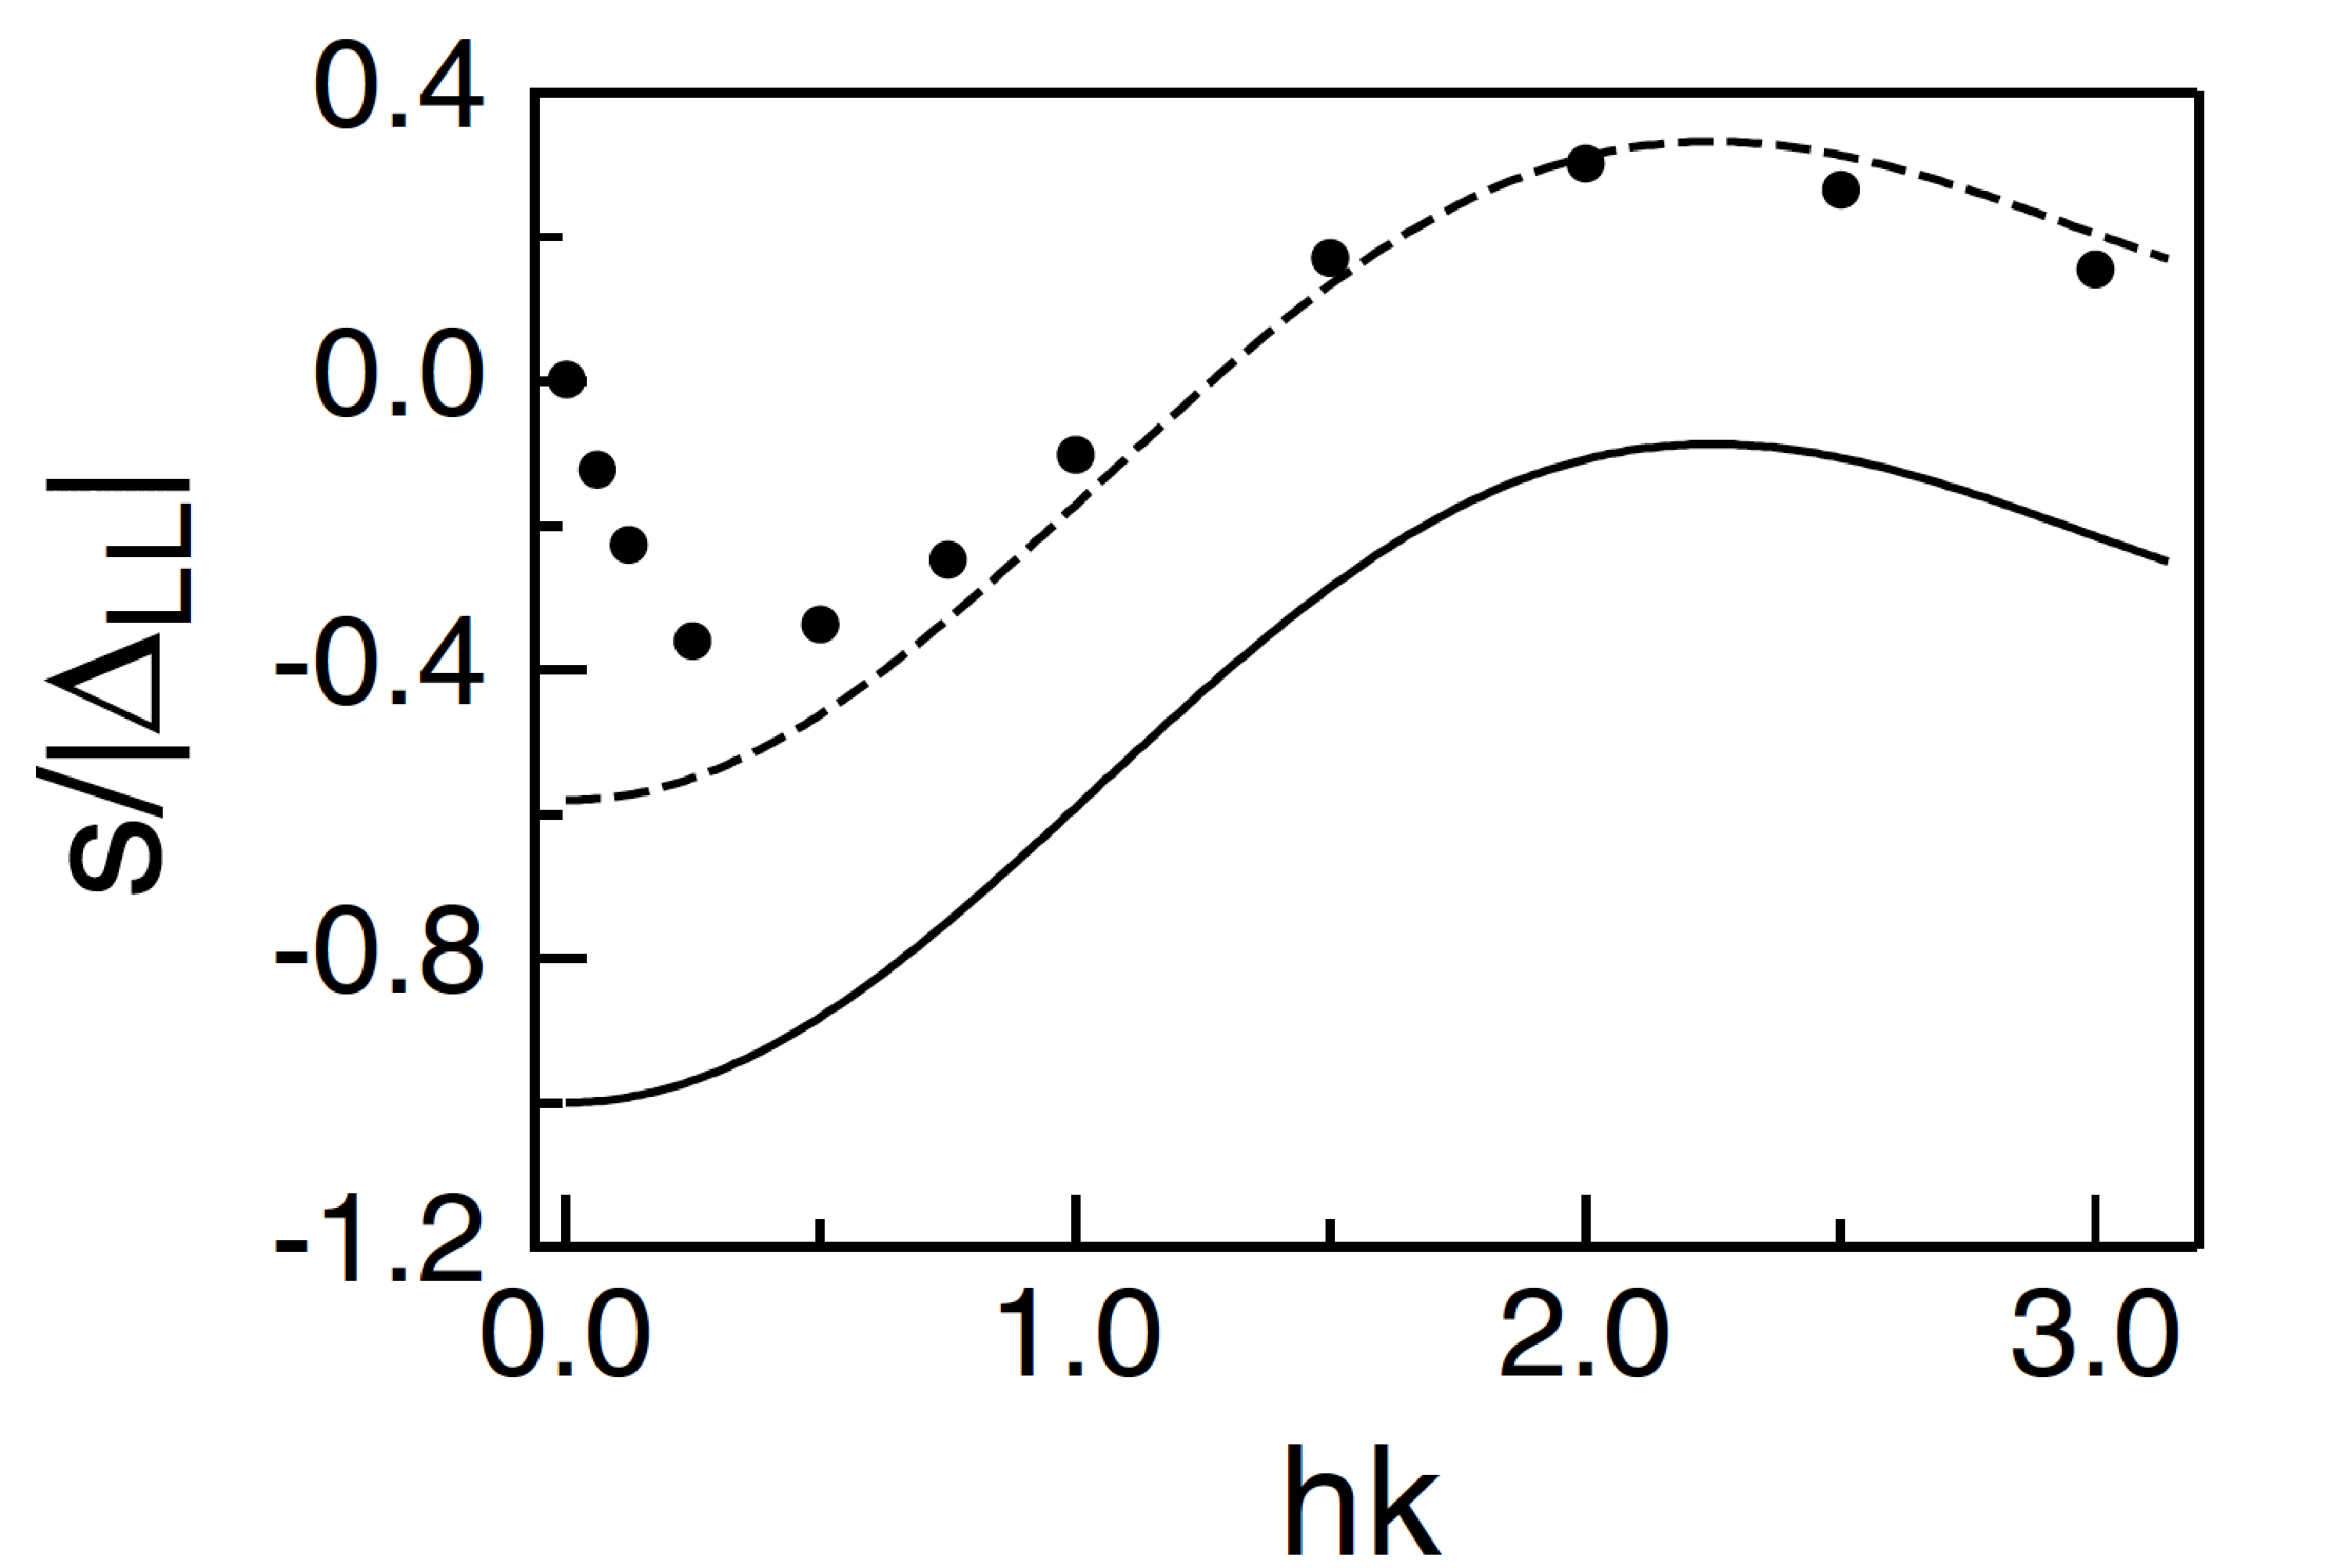
\includegraphics[width=\textwidth]{CLS_static.pdf}
\end{center}
\caption{The shift of the absorption line $s$ plotted as a function of the thickness of the sample $h$ as solid circles. The statistical error bars are smaller than the size of the circles. Also shown as a solid line is the collective Lamb shift, Eq.~\eq{LL_CLS}, and as a dashed line a vertically translated version of Eq.~\eq{LL_CLS} fitted to the numerical data points with $hk\geq 1$.}
\label{STATIC_CLS}
\end{figure}

Our interpretation is that for homogeneously broadened samples the standard electrodynamics, a mean field theory, simply fails. This is because at the density $\rho=2k^2$ the atoms are so close to one other that their dipole-dipole interactions make them a strongly interacting, or strongly correlated, system. On the other hand, inhomogeneous broadening appears to promote mean field physics.

For more insights, consider two atoms 1 and 2 with possibly different resonance frequencies, and hence, different polarizabilities $\alpha_1$ and $\alpha_2$. We sketch a formal solution to Eq.~\eq{FEQ}. The field on atom 2 that is generated by the incident field and the light scattered from atom 1 is
\bea
\bE(\br_2)&=&(1-\alpha_1\alpha_2\G\G)^{-1}[\cbE_0(\br_2)+\alpha_1\G\cbE(\br_1)]\nonumber\\
&=&\cbE_0(\br_2)+\alpha_1\G\cbE_0(\br_1)+\alpha_1\alpha_2\G\G\cbE_0(\br_2)+\dots.
\eea

The second line shows the first three terms of the expansion of $(1-\alpha_1\alpha_2\G\G)^{-1}$, with $\G\equiv\G(\br_1-\br_2)=\G(\br_2-\br_1)$. The first term is the free field on atom 2; in the second term the free field excites atom 1, which sends its dipolar field back on atom 2; in the third term the free field excites atom 2, which sends a dipolar field to excite atom 1, which sends a dipolar field back on atom 2. Further terms in the expansion come out in the same way reflecting repeated photon exchanges between the atoms. Such recurrent scattering processes in which a classical wave scatters more than once from the same atom is responsible for the cooperative phenomena and the emergence of subradiant and superradiant resonances~\cite{PhysRevA.55.513,PhysRevA.86.031602,PhysRevB.86.085116}.

Let us now regard atom 2 as the spectator and imagine averaging over the position of atom 1. Upon averaging, the second term becomes the mean-field contribution radiated by an assumedly continuous polarization, and further terms represent repeated photon exchanges between the atoms. 

Next, add the inhomogeneous broadening $\omega_D$. To the order of magnitude, averaging over the resonant frequencies suppresses the polarizability by a factor of $\gamma/\omega_D$. Thus, the first nontrivial term in the expansion corresponding to the mean-field polarization becomes suppressed by this factor, and the higher terms by higher powers of the small quantity $\gamma/\omega_D$. Qualitatively, repeated photon exchanges are deemphasized because in such processes both the emitter and the absorber are off resonance. This leaves the mean field as the dominant contribution.

Analogously, the transition from homogeneously broadened to inhomogeneously broadened phenomenology also takes place in a many-atom sample when the inhomogeneous broadening $\omega_D$ and the effective linewidth $\Gamma$ are comparable. This is, in fact, what we observe in the numerical experiments.

From classical-electrodynamics simulations, we have found qualitative features in the optical response of a homogeneously broadened dense atomic sample that are at variance with the time-honored pictures of local-field corrections and collective Lamb shifts. However, an inhomogeneous broadening, random distribution of atomic resonance frequencies, restores the agreement with the traditional theory at least in part.

So far, the simulations are based on atoms fixed in their positions, with at best a crude model for inhomogeneous broadening. In the following chapter, the actual motion of the atoms will be introduced into the simulations.


\chapter{Gases of Moving Atoms}
In experiments, the motion and collisions of the atoms is another important factor that might impact the optical response of the gas. We have to face the possibility that the influence from the kinematics of the atoms could be so prominent that some cooperative effects may be more or less eliminated. It is worthwhile to extend our simulations to moving atoms. In fact, subsequent to the simulations of inhomogeneously broadened stationary atomic samples, we develop a code to deal with the atomic motion and the associated time evolution of the dipole moments. 

Inhomogeneous broadening is included in the simulations of moving atoms as it is a natural consequence of the thermal velocity distribution of the atoms. In the stationary-atom model, given a certain spatial distribution of the atoms, we are able to solve a closed set of linear equations to obtain the dipole moment of each atom.  However, in the moving-atom model, we integrate the equation of motion of each atom's dipole moment until the gas reaches a steady state, and beyond. During that time, atoms undergo free flight as well as elastic collisions with the container walls and other atoms. Accordingly, we find that some kinematic factors such as the frequency of collisions may affect the simulation outcomes.

As expected, some results of stationary-atom simulations are inherited by moving-atom simulations, such as a dependence of collective Lamb shift on the sample thickness. Beyond that, some new features that do not exist in stationary-atom model emerge. For instance, a typical Dicke narrowed lineshape~\cite{PhysRev.89.472} is observed.

However, contrary to what one might expect, as the gas density increases, the width of the Dick-narrowed central peak increases. This is quite unlike what would happen in a hypothetical gas of independent atoms, where, if anything, a higher density should lead to a reduced Dicke-narrowed linewidth. We attribute this broadening to the strong dipole-dipole interactions between the atoms, or from an overall perspective, to cooperative response of the gas to light. 

The following discussion is organized similarly as the preceding chapter on stationary atoms. We start from the analysis of one single moving atom, extend to many independent atoms, and finally focus on atoms with dipole-dipole interactions. Of course, the calculations and simulations are again done for a circular slab.

\section{Analysis of a one-atom gas}
In our model of discrete dipolar radiators, Eq.~\eq{CORE} can be specified so that it describes the time evolution of each atom's dipole moment. For the $n$th atom located at $\mathbf{r}_n$, we have
\bea
\dot{\mathbf{d}}(\mathbf{r}_n)&=&(i\Delta-\gamma)\mathbf{d}(\mathbf{r}_n)+i\zeta\mathbf{\mathcal{E}}_0(\mathbf{r}_n)+i\zeta\sum_{m\neq n}\mathsf{G}(\mathbf{r}_n-\mathbf{r}_m)\mathbf{d}(\mathbf{r}_m).
\label{DIPOLEEQ}
\eea
As before, $\Delta=\omega-\omega_0$ is the detuning from the atomic resonance $\omega_0$, $\gamma$ is the HWHM line width of the transition, $\zeta=\mathcal{D}^2/\hbar$ and $\mathcal{D}$ is the dipole matrix element, and $\mathbf{\mathcal{E}}_0$ is the electric field of the driving light if the matter were absent. $\mathsf{G}(\mathbf{r}_n-\mathbf{r}_m)$ is the dipole field propagator from the atom at $\mathbf{r}_m$ to the atom at $\mathbf{r}_n$. Atomic motion is taken into account in that the coordinates $\mathbf{r}_n$ change with time as the atoms move.

The first term on the right hand side of Eq.~\eq{DIPOLEEQ} comes from the damped free evolution of the atomic dipole. The second and the third terms, respectively, correspond to the dipole moment induced by the incident light and by the light scattered  from all other atoms. Evidently, if the left-hand side of Eq.~\eq{DIPOLEEQ} equaled zero, this equation would give the steady state as in Eq.~\eq{STEADY}.

All the calculations and simulations we present below are done under these universal conditions:
First, the gas sample is inside a circular disk with thickness $h$ and radius $R$. For convenience, the disk is placed so that its axis is used as the $z$ axis, and the body center is the coordinate origin. Unless explicitly stated otherwise, the area and radius of the disk are $A=256$ and $R=\sqrt{256/\pi}$.
Second, the incident light is represented by $\mathcal{E}_0(\mathbf{r})=E_0\,\hat{\mathbf{e}}\,e^{i\mathbf{k}\cdot\mathbf{r}}$. It is circularly polarized and propagates in the $+z$ direction,
\bea
\hat{\mathbf{e}}=-\{\frac{1}{\sqrt{2}},\frac{i}{\sqrt{2}},0\}, \, \mathbf{k}=\{0,0,1\}.
\eea
Third, the absorption spectrum is again investigated by calculating the optical thickness $D$ of the atomic sample as explained in Ref~\cite{0953-4075-44-19-195006}. 
Fourth, as some of the analytical expressions start swelling in size, we again resort to special units such that
\bea
k=c=\hbar=\frac{1}{4\pi\epsilon_0}=1;\quad \mathcal{D}=\sqrt{\frac{3\gamma}{2}}.
\label{UNITCONVENTION}
\eea 
These are also the units that are universally used in the numerical work.

\subsection{Dipole evolution of one atom}
\label{ONEATOMDIPOLE}
If the gas consists of only one atom, Eq.~\eq{DIPOLEEQ} can be reduced to an extraordinarily simple-looking inhomogeneous first-order ODE. Even if~\eq{UNITCONVENTION} already sets the units for all physical quantities, we introduce the added scaling of the running time that it is expressed in units of $\gamma^{-1}$, and find
\bea
\dot{\mathbf{d}}(t)+(1-i\delta)\mathbf{d}(t)=i\frac{3}{2}\mathcal{E}_0(t)=i\frac{3}{2}E_0\,\hat{\mathbf{e}}\,e^{i\mathbf{k}\cdot\mathbf{r}(t)}.
\label{SINGLEEQ}
\eea
Once more we define $\delta=\Delta/\gamma$. 

For $\mathbf{k}=\{0,0,1\}$, we readily have $\mathbf{k}\cdot\mathbf{r}(t)=z(t)=z_0+v_zt$. Thus, the radial components of the initial position and velocity have no effect on the evolution of the dipole. Likewise, we need not concern ourselves with elastic collisions between the atom and the lateral surfaces of the disk. As we will see in a moment, even the initial position $z_0$ is eventually irrelevant. Therefore, we endow the atom with the initial position $\mathbf{r}_0=\{0,0,-h/2\}$ and velocity $\mathbf{v}_0=\{0,0,v\}$ to carry out our analysis. This atom is sufficient to represent all the atoms that have the same axial speed $v$. For the time being $v$ must be positive, because as the atom is initially at $z=-h/2$, it has to move in the $+z$ direction to stay inside the disk.

We may take, for instance, 
\beq
\mathbf{d}_0=-\frac{3}{2(i+\delta)}E_0e^{-i\frac{h}{2}}\hat{\mathbf{e}}
\eeq
 as the initial dipole moment for the evolution, although the steady state that the dipole reaches after a long time is independent of the initial state as well. Anyway, given ${\bf d}_0$, the solution to Eq.~\eq{SINGLEEQ} is
\bea
d(t)&=&-\frac{3E_0}{2(i+\delta-v)}e^{i(-h/2+vt)}\left[1-e^{-t+i(\delta-v)t}\right]+e^{-t+i\delta t}d_0\,.
\label{SINGLESOL}
\eea
Note that we do not use the bold font anymore because the dipole moment always has the same polarization as the incoming electric field. The polarization $\hat{\mathbf{e}}$ can then be eliminated from the equation and everything is scalar.

Obviously, the first term in Eq.~\eq{SINGLESOL} depends on the velocity on and the instantaneous electric field at the ever-changing position of the atom. The second term conveys the damping of the initial dipole. In free space, as time tends to infinity, the dipole moment would asymptotically approach
\bea
d(t\to\infty)=\alpha(v)E_0e^{i(-h/2+vt)},
\eea
where
\beq
\alpha(v)=-\frac{3}{2(i+\delta-v)}
\eeq
 is the Doppler-shifted polarizability of the atom with the speed $v$.

However, the atom is confined to the disk. In our model it experiences elastic collisions with the end caps of the disk at $z=\pm h/2$, whereupon the direction of the velocity reverses. The time interval between any two successive collisions is $h/v$. At the time $h/v$ the first collision happens at $z=h/2$, and the dipole is
\bea
d_1\equiv d(t=\frac{h}{v})&=&\alpha(v)E_0 e^{ih/2}\left[1-e^{-\frac{h}{v}+i(\delta-v)\frac{h}{v}}\right]+e^{-\frac{h}{v}+i\delta \frac{h}{v}}d_0.
\eea
$d_1$ would in turn serve as the initial state to obtain the dipole at the second collision, $d_2$. Note that this time $v$ is replaced by $-v$ as the atom bounces back after the first collision:
\bea
d_2&=&\alpha(-v)E_0e^{-ih/2}\left[1-e^{-\frac{h}{v}+i(\delta+v)\frac{h}{v}}\right]+e^{-\frac{h}{v}+i\delta \frac{h}{v}}d_1\nonumber\\
&=&\alpha(-v)E_0e^{-ih/2}\left[1-e^{-\frac{h}{v}+i(\delta+v)\frac{h}{v}}\right]+\alpha(v)E_0e^{ih/2}\left[1-e^{-\frac{h}{v}+i(\delta-v)\frac{h}{v}}\right]e^{-\frac{h}{v}+i\delta \frac{h}{v}}\nonumber\\
&&+(e^{-\frac{h}{v}+i\delta \frac{h}{v}})^2d_0\nonumber\\
&=&d_+q+d_-+q^2d_0.
\eea
Here we have defined
\bea
d_+&=&\alpha(v)E_0e^{ih/2}\left[1-e^{-\frac{h}{v}+i(\delta-v)\frac{h}{v}}\right],\nonumber\\
d_-&=&\alpha(-v)E_0e^{-ih/2}\left[1-e^{-\frac{h}{v}+i(\delta+v)\frac{h}{v}}\right], \nonumber\\
q&=&e^{-\frac{h}{v}+i\delta \frac{h}{v}}
\eea
for a more compact notation.

Now we can inductively write out the dipole moment at the $n$th collision as 

\begin{subequations}
\begin{numcases}{d_n=}
d_+\sum_{k=0}^{\frac{n-1}{2}}q^{2k}+d_-\sum_{k=0}^{\frac{n-3}{2}}q^{2k+1}+q^nd_0, &($n$ is odd and $n\geq 3$) \\
 \nonumber\\
d_+ \sum_{k=0}^{\frac{n-2}{2}}q^{2k+1}+d_- \sum_{k=0}^{\frac{n-2}{2}}q^{2k}+q^nd_0. &($n$ is even and $n\geq 2$)
\end{numcases}
\end{subequations}
Since $\left|q\right|<1$, the summations converge as $n\to\infty$ so that we have
\begin{subequations}
\begin{numcases}{d_{n\to\infty}=}
\frac{d_++qd_-}{1-q^2} \,, & \textrm{(odd $n$)}\label{FINAL1}\\
\nonumber\\
\frac{qd_++d_-}{1-q^2}\,. & \textrm{(even $n$)}.\label{FINAL2}
\end{numcases}
\end{subequations}
If we wait long enough, the time evolution eventually leads to an alternation of the dipole moment between the values~\eq{FINAL1} and~\eq{FINAL2} when the atom bounces off the endcaps. In steady state the dipole moment is equal to~\eq{FINAL1} when the atom arrives at the endcap at $z=h/2$ and equal to~\eq{FINAL2} when it is at $z=-h/2$.

Between the two ends of the cylinder, the dipole moment still evolves according to Eq.~\eq{SINGLESOL}. The oscillations of the dipole moment are synchronized with the kinematic oscillations. The period of both oscillations equals the duration of a round trip between the two endcaps, which is $2h/v$.

Consider the dipole moment over one period, starting the time when the atom is at $z=-h/2$. In the first half of the period the dipole moment is
\bea
d_{F}(t)&=&\alpha(v)E_0e^{ih/2}\left[1-e^{-t+i(\delta-v)t}\right]+q(qd_++d_-)\frac{1}{1-q^2}.
\label{FORWARD}
\eea
We zero the timer again when the atom reaches $z=h/2$, so that during the return trip the dipole is
\bea
d_{B}(t)&=&\alpha(-v)E_0e^{-ih/2}\left[1-e^{-t+i(\delta+v)t}\right]+q(d_++qd_-)\frac{1}{1-q^2}.
\label{BACKWARD}
\eea
Combining Eq.~\eq{FORWARD} and Eq.~\eq{BACKWARD}, we are able to write out the dipole moment at any time within one period,
\begin{numcases}{d(t)=}
d_F(t), & ($0\leq t\leq  h/v$)\nonumber\\
d_B(t-h/v). & ($h/v \leq t \leq 2h/v)$
\label{BACKFORTH}
\end{numcases}

\subsection{Optical thickness}
For the present purposes let us write the optical thickness as $D=-\ln|\tau|^2$,
where $\tau$ is the amplitude transmission coefficient. Now, compared with all other time scales of the problem, the propagation of the light across the disk is typically instantaneous. We may therefore define an instantaneous amplitude transmission coefficient and optical thickness as well. We again use the forward-scattering approximation of Ref.~\cite{1367-2630-14-5-055001}, see Eq.~\eq{TRLIGHT} and also Ref.~\cite{0953-4075-44-19-195006}. The dipole moment is actually an explicit function of $h$, $v$, $\delta$ and $t$, so we write it as $d(h,v,\delta,t)$, and have the amplitude transmission coefficient for a single atom
\bea
\tau_1=1+\frac{2ie^{-iz(t)}d(h,v,\delta,t)}{R^2E_0},
\eea
where $z(t)$ is the position of the atom at time $t$. The phase of this transmission coefficient is referenced to $z=0$; multiply by $e^{ih/2}$ for the amplitude transmission coefficient at the exit face of the disk.

The optical thickness $D_1$ is
\bea
D_1(h,v,\delta,t)&=&\ln\left|\tau_1\right|^{-2}=-\ln\left|\tau_1\right|^2=-\ln(\tau_1\tau_1^*)\nonumber\\
&=&-\ln\Bigg\{1+2\,\mathfrak{R}\left[\frac{2ie^{-iz(t)}}{R^2}\frac{d(h,v,\delta,t)}{E_0}\right]\nonumber\\
&&+\left|\frac{2ie^{-iz(t)}}{R^2}\frac{d(h,v,\delta,t)}{E_0}\right|^2\Bigg\}.
\eea
For $R\gg1$, we have the approximation
\bea
D_1(h,\delta,v,t)&\approx&-\ln\left(1+2\,\mathfrak{R}\left[\frac{2ie^{-iz(t)}}{R^2}\frac{d(h,v,\delta,t)}{E_0}\right]\right)\nonumber\\
&\approx&-\frac{4}{R^2E_0}\mathfrak{R}\left[ie^{-iz(t)}d(h,v,\delta,t)\right].
\label{APPROX}
\eea

As we discussed in Sec.~\ref{ONEATOMDIPOLE}, $z(t)$ and $d(h,v,\delta,t)$ are oscillating in phase, so the time average of the optical thickness can be calculated by integrating the term in the square brackets over a round trip of the atom and dividing the result by the round-trip time $2h/v$,
 \bea
\bar{D}_1(h,v,\delta)&=&-\frac{4}{R^2E_0}\mathfrak{R}\left[\frac{v}{2h}\int_0^{\frac{2h}{v}} ie^{-iz(t)} d(h,v,\delta,t)dt\right]\nonumber\\
&=&\frac{4}{R^2}\mathfrak{R}\Bigg\{\frac{3v^3\left[{\rm coth}(\frac{h-ih\delta}{v})-\cos(h){\rm csch}(\frac{h-ih\delta}{v})\right]}{h(i+\delta-v)^2(i+\delta+v)^2}\nonumber\\
&&-\frac{3(1-i\delta)}{2(i+\delta-v)(i+\delta+v)}\Bigg\}.
\label{THEORYD}
\eea
As the final step, we imagine an ensemble of an infinite number of one-atom samples in which the atom's axial velocity obeys the Gaussian distribution with zero mean and rms axial velocity (standard deviation) equal to $u$. Then the ensemble-averaged absorption spectrum is
\bea
D_1(h,u,\delta)=\int_{-\infty}^{\infty}\bar{D}_1(h,v,\delta)\frac{e^{-\frac{v^2}{2u^2}}}{\sqrt{2\pi}\,u}dv.
\label{ONEATOMSPECTRUM}
\eea

We numerically compute and plot $D_1(\delta)$ versus $\delta$ in  Fig.~\ref{SINGLESPECTRUM} for certain values of $h$ and $u$. The lines are from~Eq.~\eq{ONEATOMSPECTRUM}. The markers give outcomes from the corresponding direct numerical simulations, to be explained in detail below.
\begin{figure}[h!]
\begin{center}
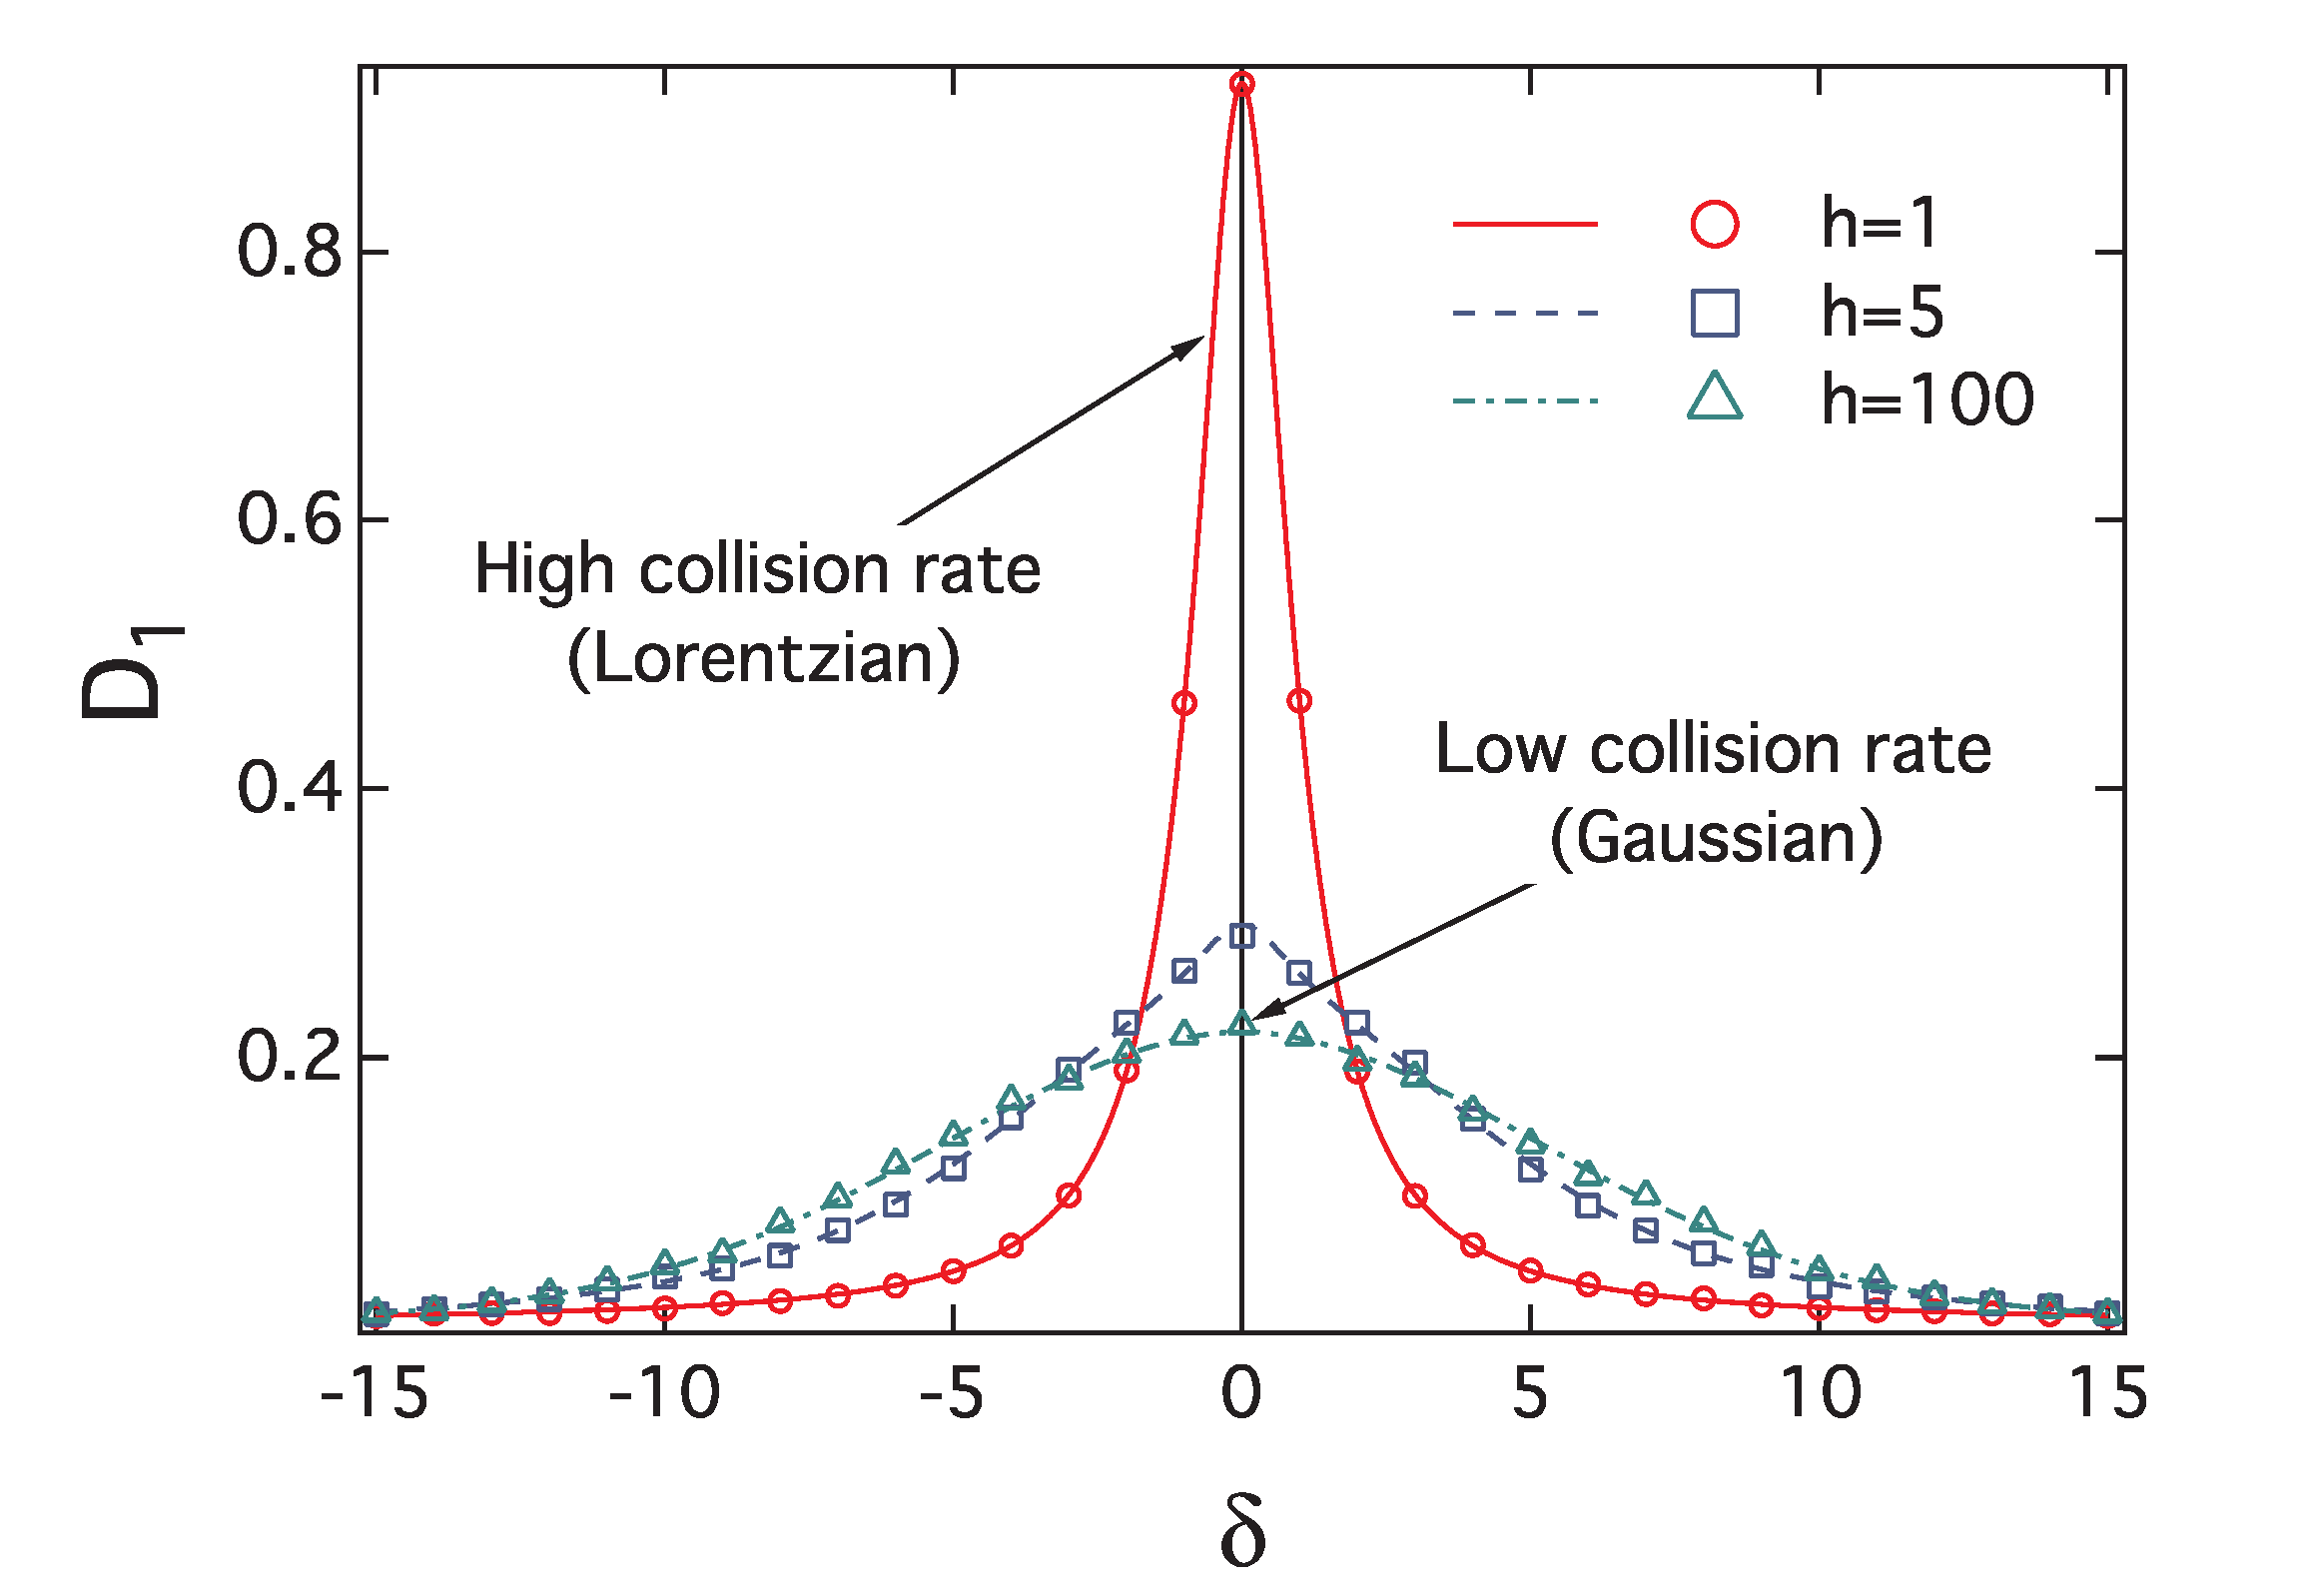
\includegraphics[width=\textwidth]{single_atom.pdf}
\end{center}
\caption{Optical thickness $D_1$ versus detuning $\delta$ of a single-atom ensemble with disk thicknesses $h=100, 5$ and $1$. The rms axial speed of the atom is $v=5$ for all of the data. Continuous lines are results from Eq.~\eq{ONEATOMSPECTRUM}, discrete markers give results from the corresponding direct numerical simulations. Essentially Gaussian and Lorentzian profiles are observed for $h=100$ and $h=1$, respectively. When $h=5$, a bulge close to resonance makes the lineshape intermediate between a Gaussian and a Lorentzian. Numerical simulations agree with the analytical calculations.}
\label{SINGLESPECTRUM}
\end{figure}

The three curves in  Fig.~\ref{SINGLESPECTRUM} reveal an important phenomenon. As we keep the rms speed of the atom constant and vary the thickness $h$ from very large to very small, the spectrum undergoes a transition from a broad Gaussian line to a narrow Lorentzian. This transition is consistent with Dicke narrowing~\cite{PhysRev.89.472}. Basically, if an atom were to fly freely in space, a situation approximated at the thickness $h=100$, such motion would add a Doppler shift to the atomic resonance frequency that can be detected spectroscopically. On the other hand, if collisions confine the atom to a small region compared to the wavelength of light, as in the case $h=1$, then the atom-field interaction is as if the atom were stationary. The case $h=5$ is intermediate between the two extreme cases, and shows an intermediate spectrum. 

\subsection{A simplified many-atom gas}
\label{SMAG}

We can make one more step forward with a simplified model of a gas of $N$ atoms.
So far the atom radius is taken to be infinitesimal, hence there are no atom-atom collisions. Moreover, the dipole-dipole interaction between the atoms is neglected, hence neither collisions as a result of the forces between the dipoles nor cooperative radiative properties occur. Under these conditions each atom evolves independently of the others, and the dipole moment of each atom in steady state is still given by Eq.~\eq{BACKFORTH}. 

If we have $\{v_n\}$ $(n=1,2,3,\cdots,N)$ as the speeds of the $N$ atoms, the total amplitude transmission coefficient can be written
\bea
\tau_N=1+\sum_{n=1}^{N}\frac{2ie^{-iz_n(t)}d(h,\delta,v_n,t)}{R^2E_0},
\eea
where $z_n(t)$ is the ever-changing position of the $n$th atom. 

Like before, we assume $R\gg 1$, so the approximation in Eq.~\eq{APPROX} is still valid and the total optical thickness of the gas is
\bea
D_N(h,\{v_n\}, \delta,t)&\approx&-\frac{4}{R^2E_0}\mathfrak{R}\left[\sum_{n=1}^{N}ie^{-iz_n(t)}d(h,\delta,v_n,t)\right]=\sum_{n=1}^{N}D_1(h,v_n,\delta,t).\nonumber\\
\eea
Note that the sum and the time integral in Eq.~\eq{THEORYD} are interchangeable, so the time average is
\bea
\bar{D}_N(h,\{v_n\},\delta)=\sum_{n=1}^{N}\bar{D}_1(h,v_n,\delta).
\eea
Finally, if all of the $v_n$ have a Gaussian distribution with the rms velocity $u$, the absorption spectrum of the N-atom gas is
\bea
D_N(h,u,\delta)=ND_1(h,u,\delta).
\eea

We can see that, except for a multiplying factor $N$, the spectrum from such a simplified model of a gas is identical to the spectrum of a single atom, as in Fig.~\ref{SINGLESPECTRUM}. 
 
This is as far as we can get analytically, up to quadrature. As we want to investigate the influence of atom-atom collisions on the spectrum next, we have to turn to simulations.

The details of our simulations will be explained in next section. Here, as a preview, we present simulation results for a gas of $N$ atoms with and without atom-atom collisions in Fig.~\ref{COLLISION}. However, dipole-dipole interactions are still not included in either analytical results or in numerical simulations. It is clear that, as we adopt a large atom radius so that atom-atom collisions become prevalent, the line shape significantly narrows.

\begin{figure}[h!]
\begin{center}
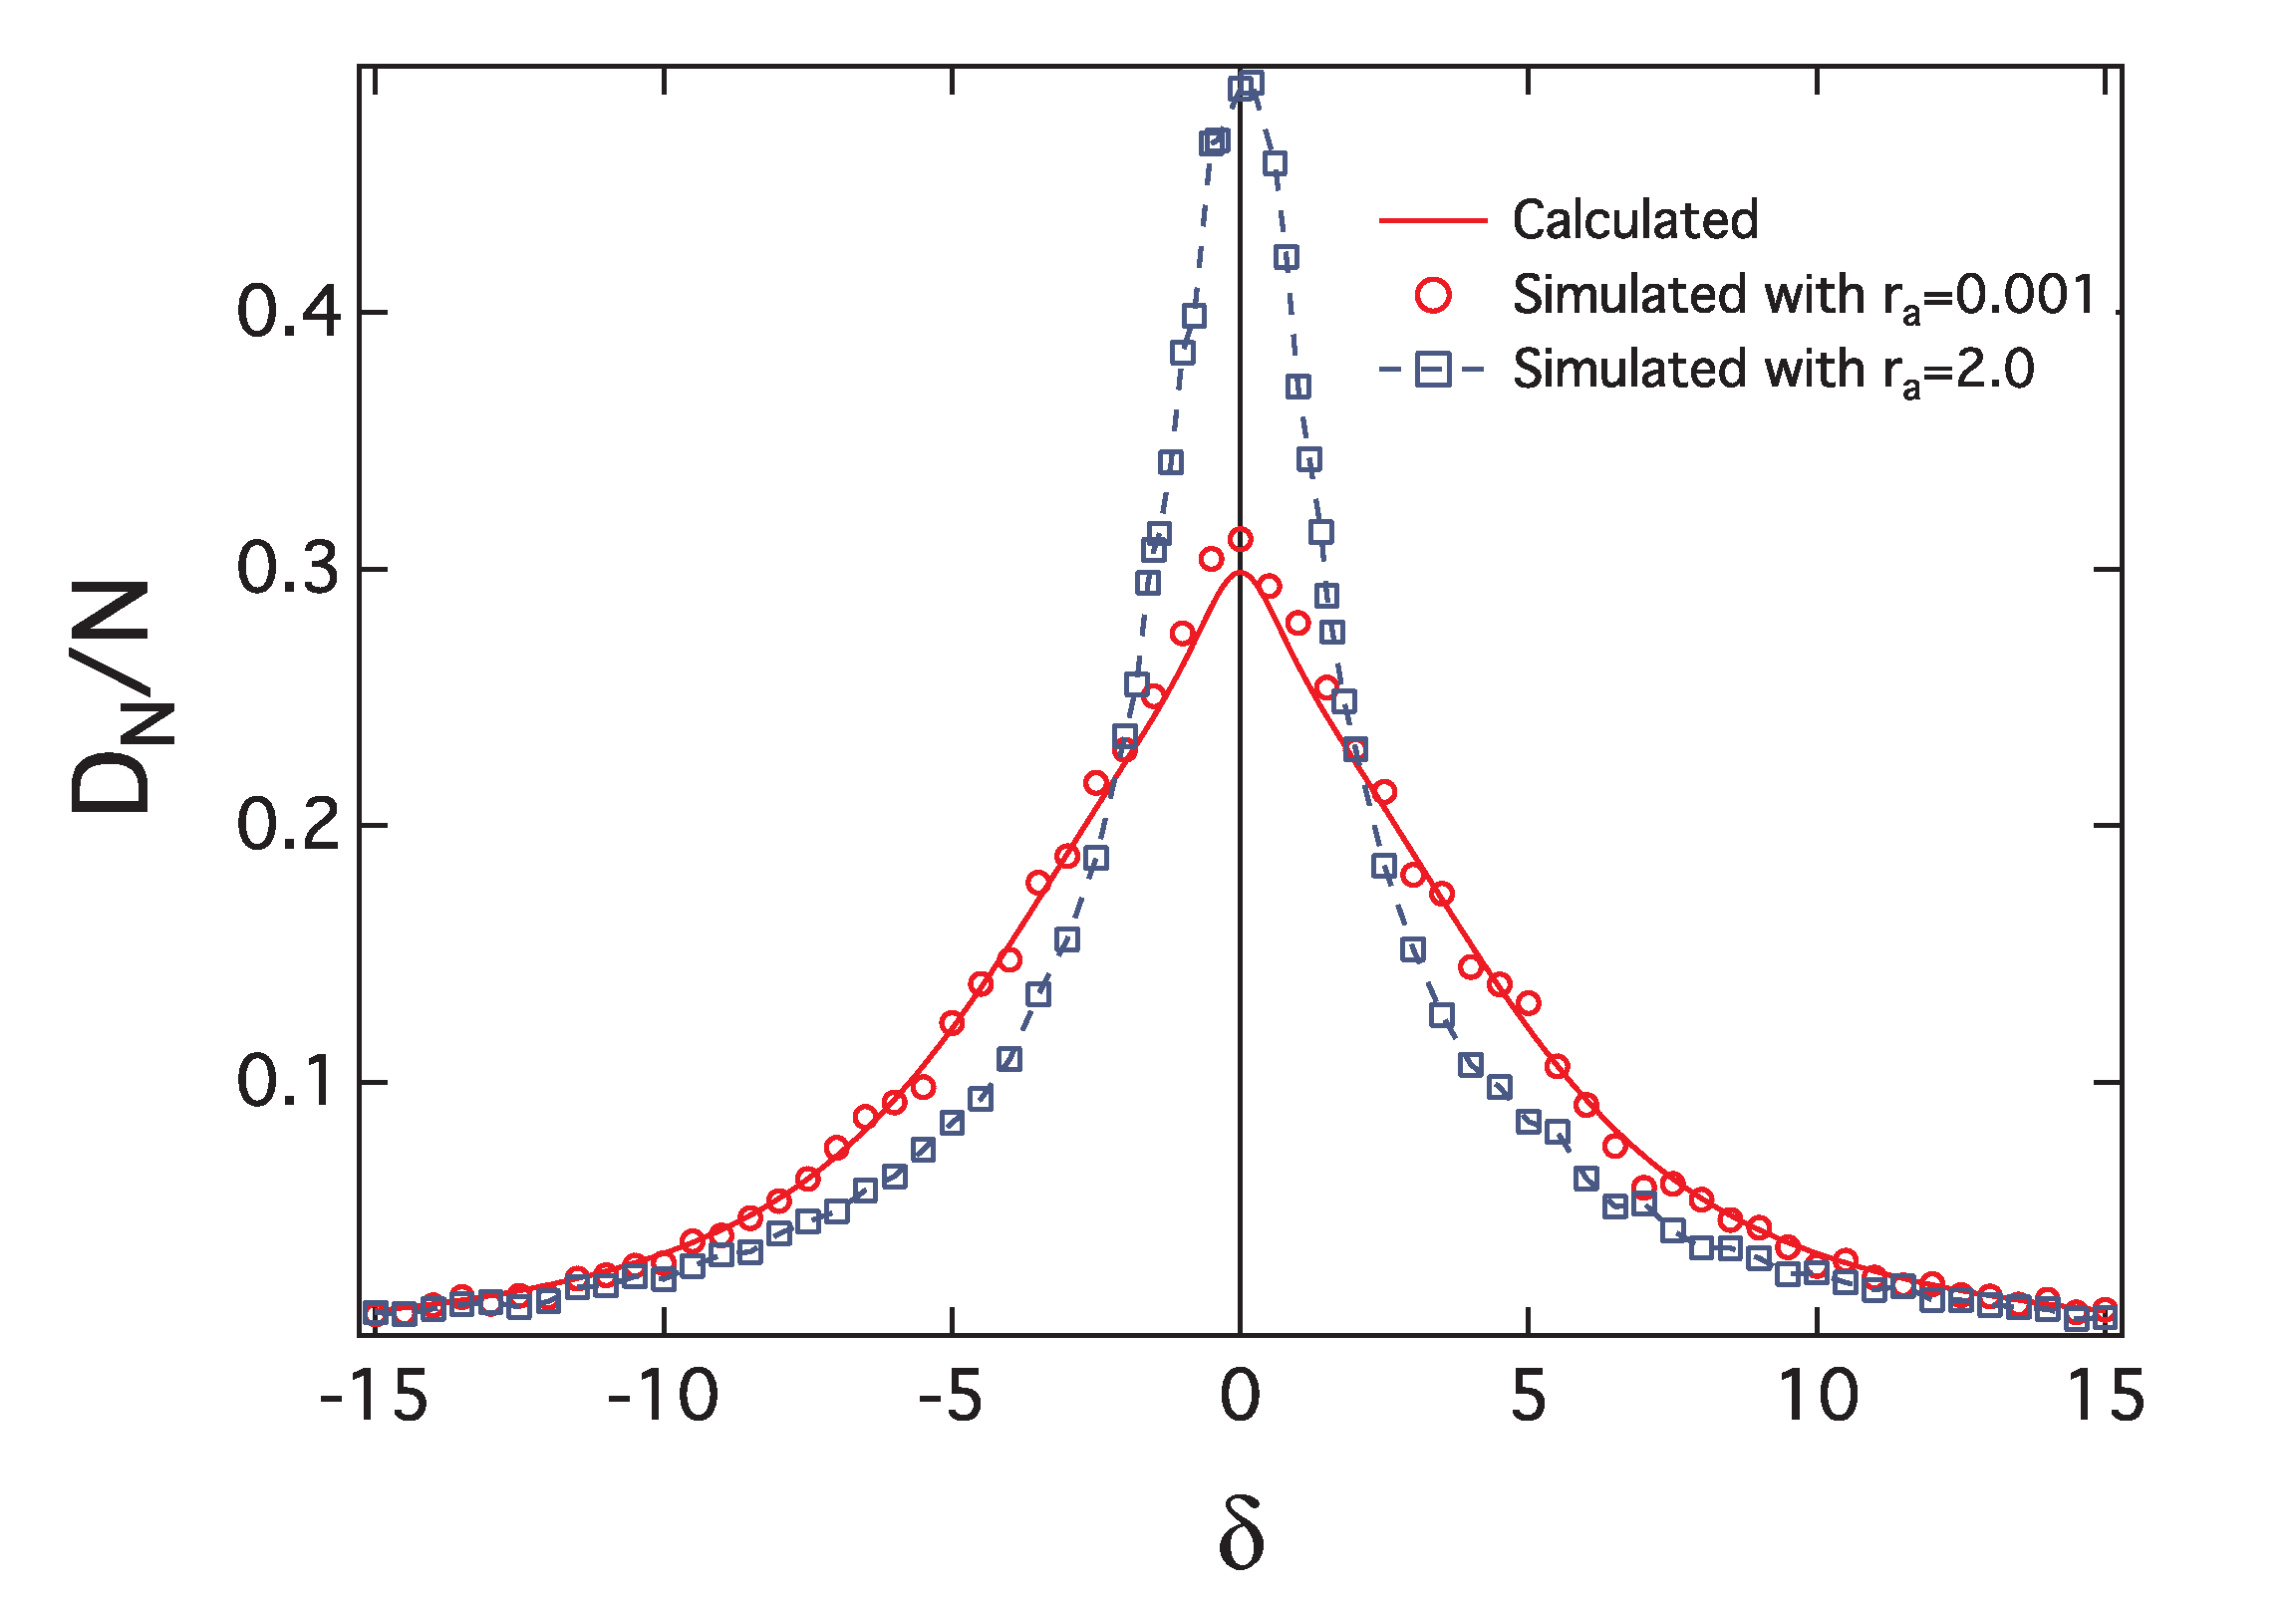
\includegraphics[width=\textwidth]{COLLISION.pdf}
\end{center}
\caption{Optical thickness per atom $D_N/N$ versus detuning from resonance $\delta$ with different atom-atom collision rates if there were no dipole-dipole interactions. The solid line is from Eq.~\eq{ONEATOMSPECTRUM}, and is identical to $D_1$ with $h=5$ in Fig.~\ref{SINGLESPECTRUM}. The red circles correspond to simulations where the atom radius was $r_a=0.001$, and the simulation programs recorded no atom-atom collisions at all. The blue boxes are for simulations with $r_a=2.0$, so about half of the collisions of the atoms are mutual collisions and half are collisions with the walls of the container. In all cases, $N=10$, $u=5$, $R=\sqrt{256/\pi}$ and $h=5$.}
\label{COLLISION}
\end{figure}
In summary, if the dipole-dipole interactions between the atoms were completely absent, either by shortening the disk in the $z$-direction or by increasing the atom radius we would end up with a narrowing lineshape in the absorption spectrum. The essential mechanism is the same in both cases: the mean free path of the atoms is reduced and the resulting confinement leads to Dicke narrowing.

\section{Simulations of many-atom gases}
\subsection{Procedure and validity of the simulation program}

Most of our effort is put into simulations that include the dipole-dipole interactions. Some details about the simulations will first be discussed. 

\subsubsection{Initial state of the evolution}

We assume that, initially, the gas sample is evenly distributed inside the circular disk. The atoms obey the Maxwell-Boltzmann velocity distribution and have the same root-mean-square velocity in all three orthogonal directions.

Although the initial dipole moments of the atoms are irrelevant to the eventual steady state, it is still worthwhile to choose the initial state carefully so that the system relaxes to the steady state as quickly as possible. This is critical when we deal with a large number of atoms. The efficiency of the computations becomes a major concern, especially as this numerical problem is not a good match to the paradigm underlying Open Science Grid.

In our simulations, after the initializations of the positions and velocities, the first step is to solve the same equations for the dipole moments of the atoms as in a stationary-atom simulation with inhomogeneous broadening. The resonance frequency of each atom is simply Doppler-shifted by $\Delta\omega=kv_z$. The solutions to these $6N$ linear equations provide the initial state for the dipole evolution described by Eq.~\eq{DIPOLEEQ}.

\subsubsection{Integration of the evolution equations and sampling}

We use adaptive-stepsize Runge-Kutta method to integrate Eq.~\eq{DIPOLEEQ} numerically. The coordinates of the $n$th atom $\mathbf{r}_n$ change with time as the atom moves. Between two successive collisions, the displacement of all atoms is linear to time. However, this linear dependence is interrupted by collisions.

As to collisions, an atom is conceptually treated as hard sphere with the radius $r_a$. Each atom may collide either with another atom, or with the inside wall of the container. All collisions are assumed elastic. Again conceptually (implementations may differ on this), we artificially enlarge the stated radius and thickness of the disk, 
$R\rightarrow R+r_a$ and $h\rightarrow h+2r_a$, so that the center-of-mass of each atom has the entire volume $\pi R^2h$ available.

In more algorithmic detail, we use the data structures available in the Standard Template Library of C++ to maintain a record (a ``map'' in one particular implementation) of the next known collision for each atom: when and where will it happen and whether it is an atom-atom collision or a collision with a container wall. The atom that collides first obviously determines the next collision overall. At a collision, both the atomic velocities and the record of the next known collision for each atom are updated appropriately. Between the collisions, the atoms simply fly ballistically. This algorithm has proven to be very efficient. In the cases when we have profiled the code, it has spent most of the time computing the dipole-dipole interactions.

When a collision happens, we halt the Runge-Kutta integration, update the atom or atoms that just collided with the new velocity or velocities, and then resume the integration.

It may be noted that we have also studied the motion of the atoms with the collisions but without integrating the dipole moments. This is in order to test the system that manages the motion of the atoms. The results have been satisfactory. For instance, we have seen a monoenergetic distribution of atomic velocities relax to a Maxwell-Boltzmann velocity distribution as anticipated.

In the simulations with stationary atoms we take the average over many statistically independent static samples. Now we may also work with time averages in one sample.  We wait for a time much longer (say, ten times longer) than the relaxation time of the system to reach a steady state, and then begin to take snapshots of the quantity we wish to analyze. The time interval between the snapshots should also be longer than the relaxation time to ensure the statistical independence of the samples. Each snapshot works as a sample in our analysis. 

The caveat here is that the relaxation time has proven difficult to determine. One could, for instance, start the system from a state far from equilibrium and follow the optical thickness relax to a constant. Alternatively, one could analyze the fluctuations of the samples in the purported steady state as a function of the time interval between the samples to get an idea of the statistical independence of the samples. The unfortunate fact is that the results for the relaxation time from such different methods may easily differ by an order of magnitude.

\subsubsection{Collective Lamb shift for moving atoms}
 
In the simulations with stationary atoms, collective Lamb shifts are observed in dense gases when inhomogeneous broadening is added. Figure~\ref{CLS} correspondingly shows similar oscillations of the shift of the resonance as a function of sample thickness from theory, Eq.~\eq{LL_CLS} (solid line), and from simulations with moving atoms (filled circles). The dashed line is a vertically translated version of the theory. We emphasize that, no matter whether in the experiments~\cite{PhysRevLett.108.173601}, in stationary-atom simulations ~\cite{PhysRevLett.112.113603} or in the present moving-atom simulations, an additive constant is always needed to match the data points and theory.  The atom number we have used was limited to at most $N=768$, as our simulations are constrained by the available computer capacity. 

\begin{figure}[h!]
\begin{center}
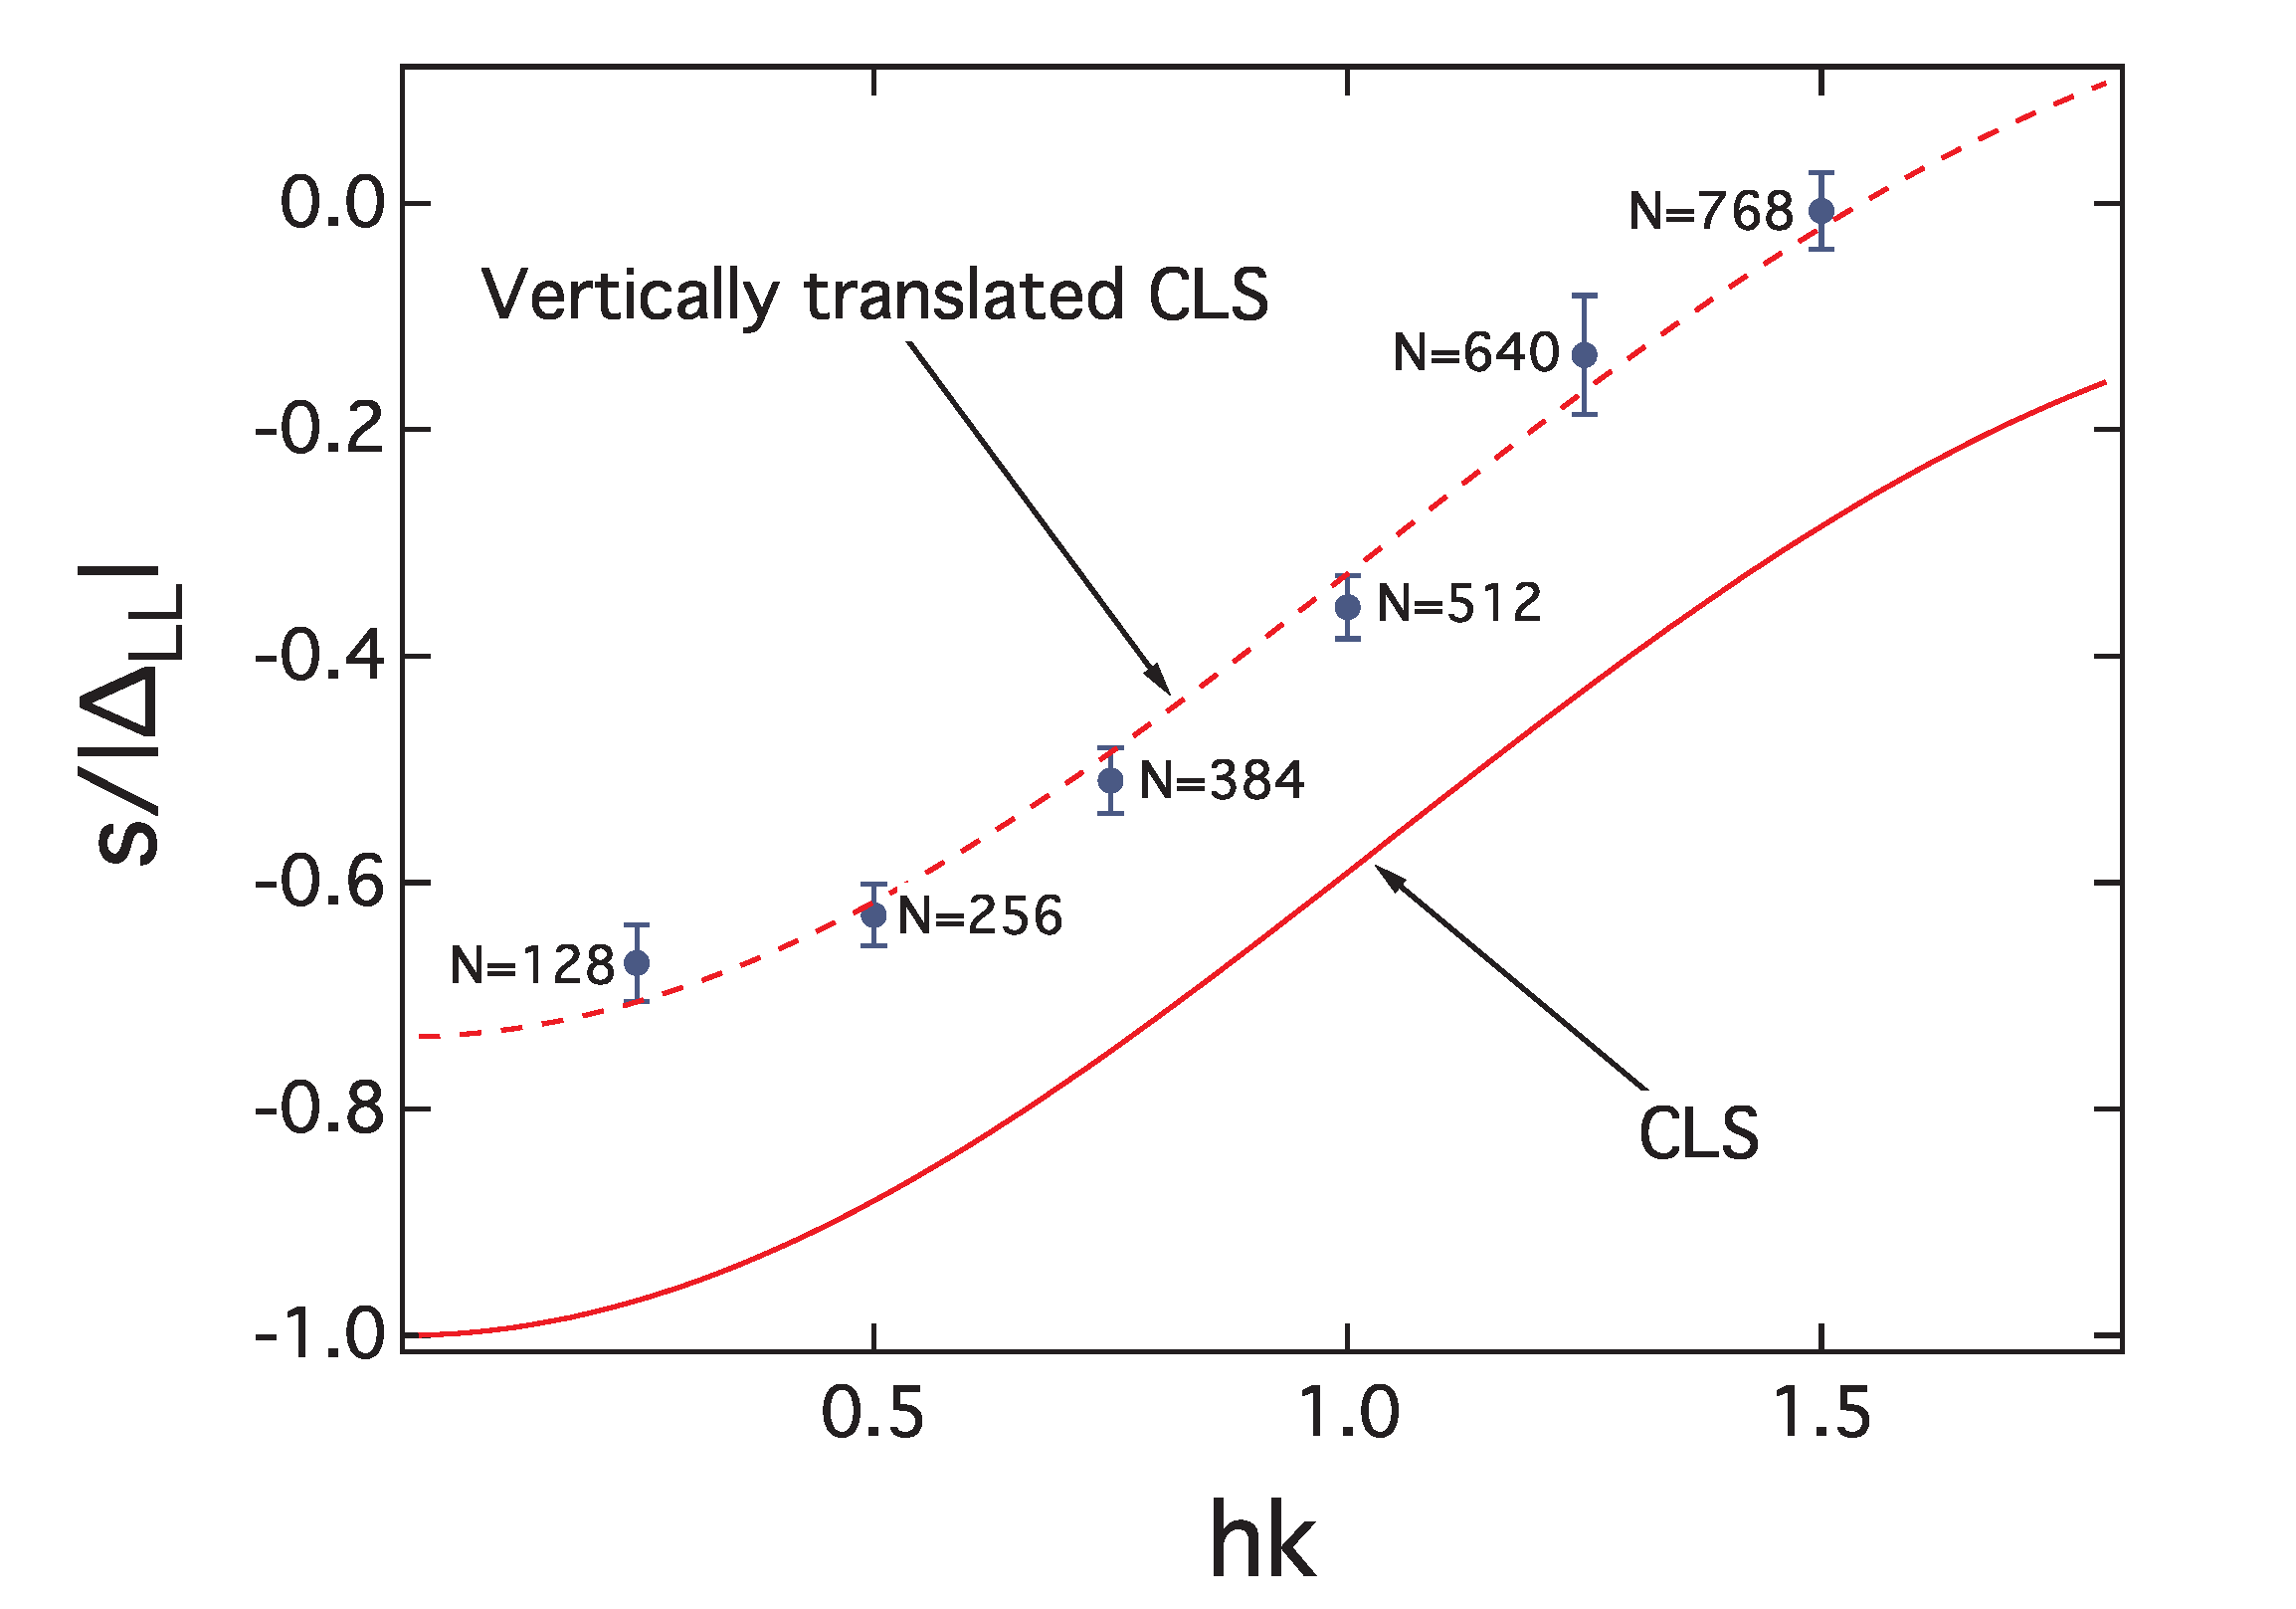
\includegraphics[width=\textwidth]{CLS.pdf}
\end{center}
\caption{The shift of the absorption line $s$ versus the thickness $h$ in a dense gas of moving atoms. $\Delta_{LL}$ is the standard LL shift. The shift is defined as shift of fitted Lorentzian.  The fixed parameters are $\rho=2$, $A=256$, and $u=500$.}
\label{CLS}
\end{figure}

\subsection{Broadening of the Dicke-narrowed lineshape in a dense gas}

By varying the density of the gas, we found new signs of cooperative effects in the absorption spectra.

\begin{figure}[h!]
\begin{center}
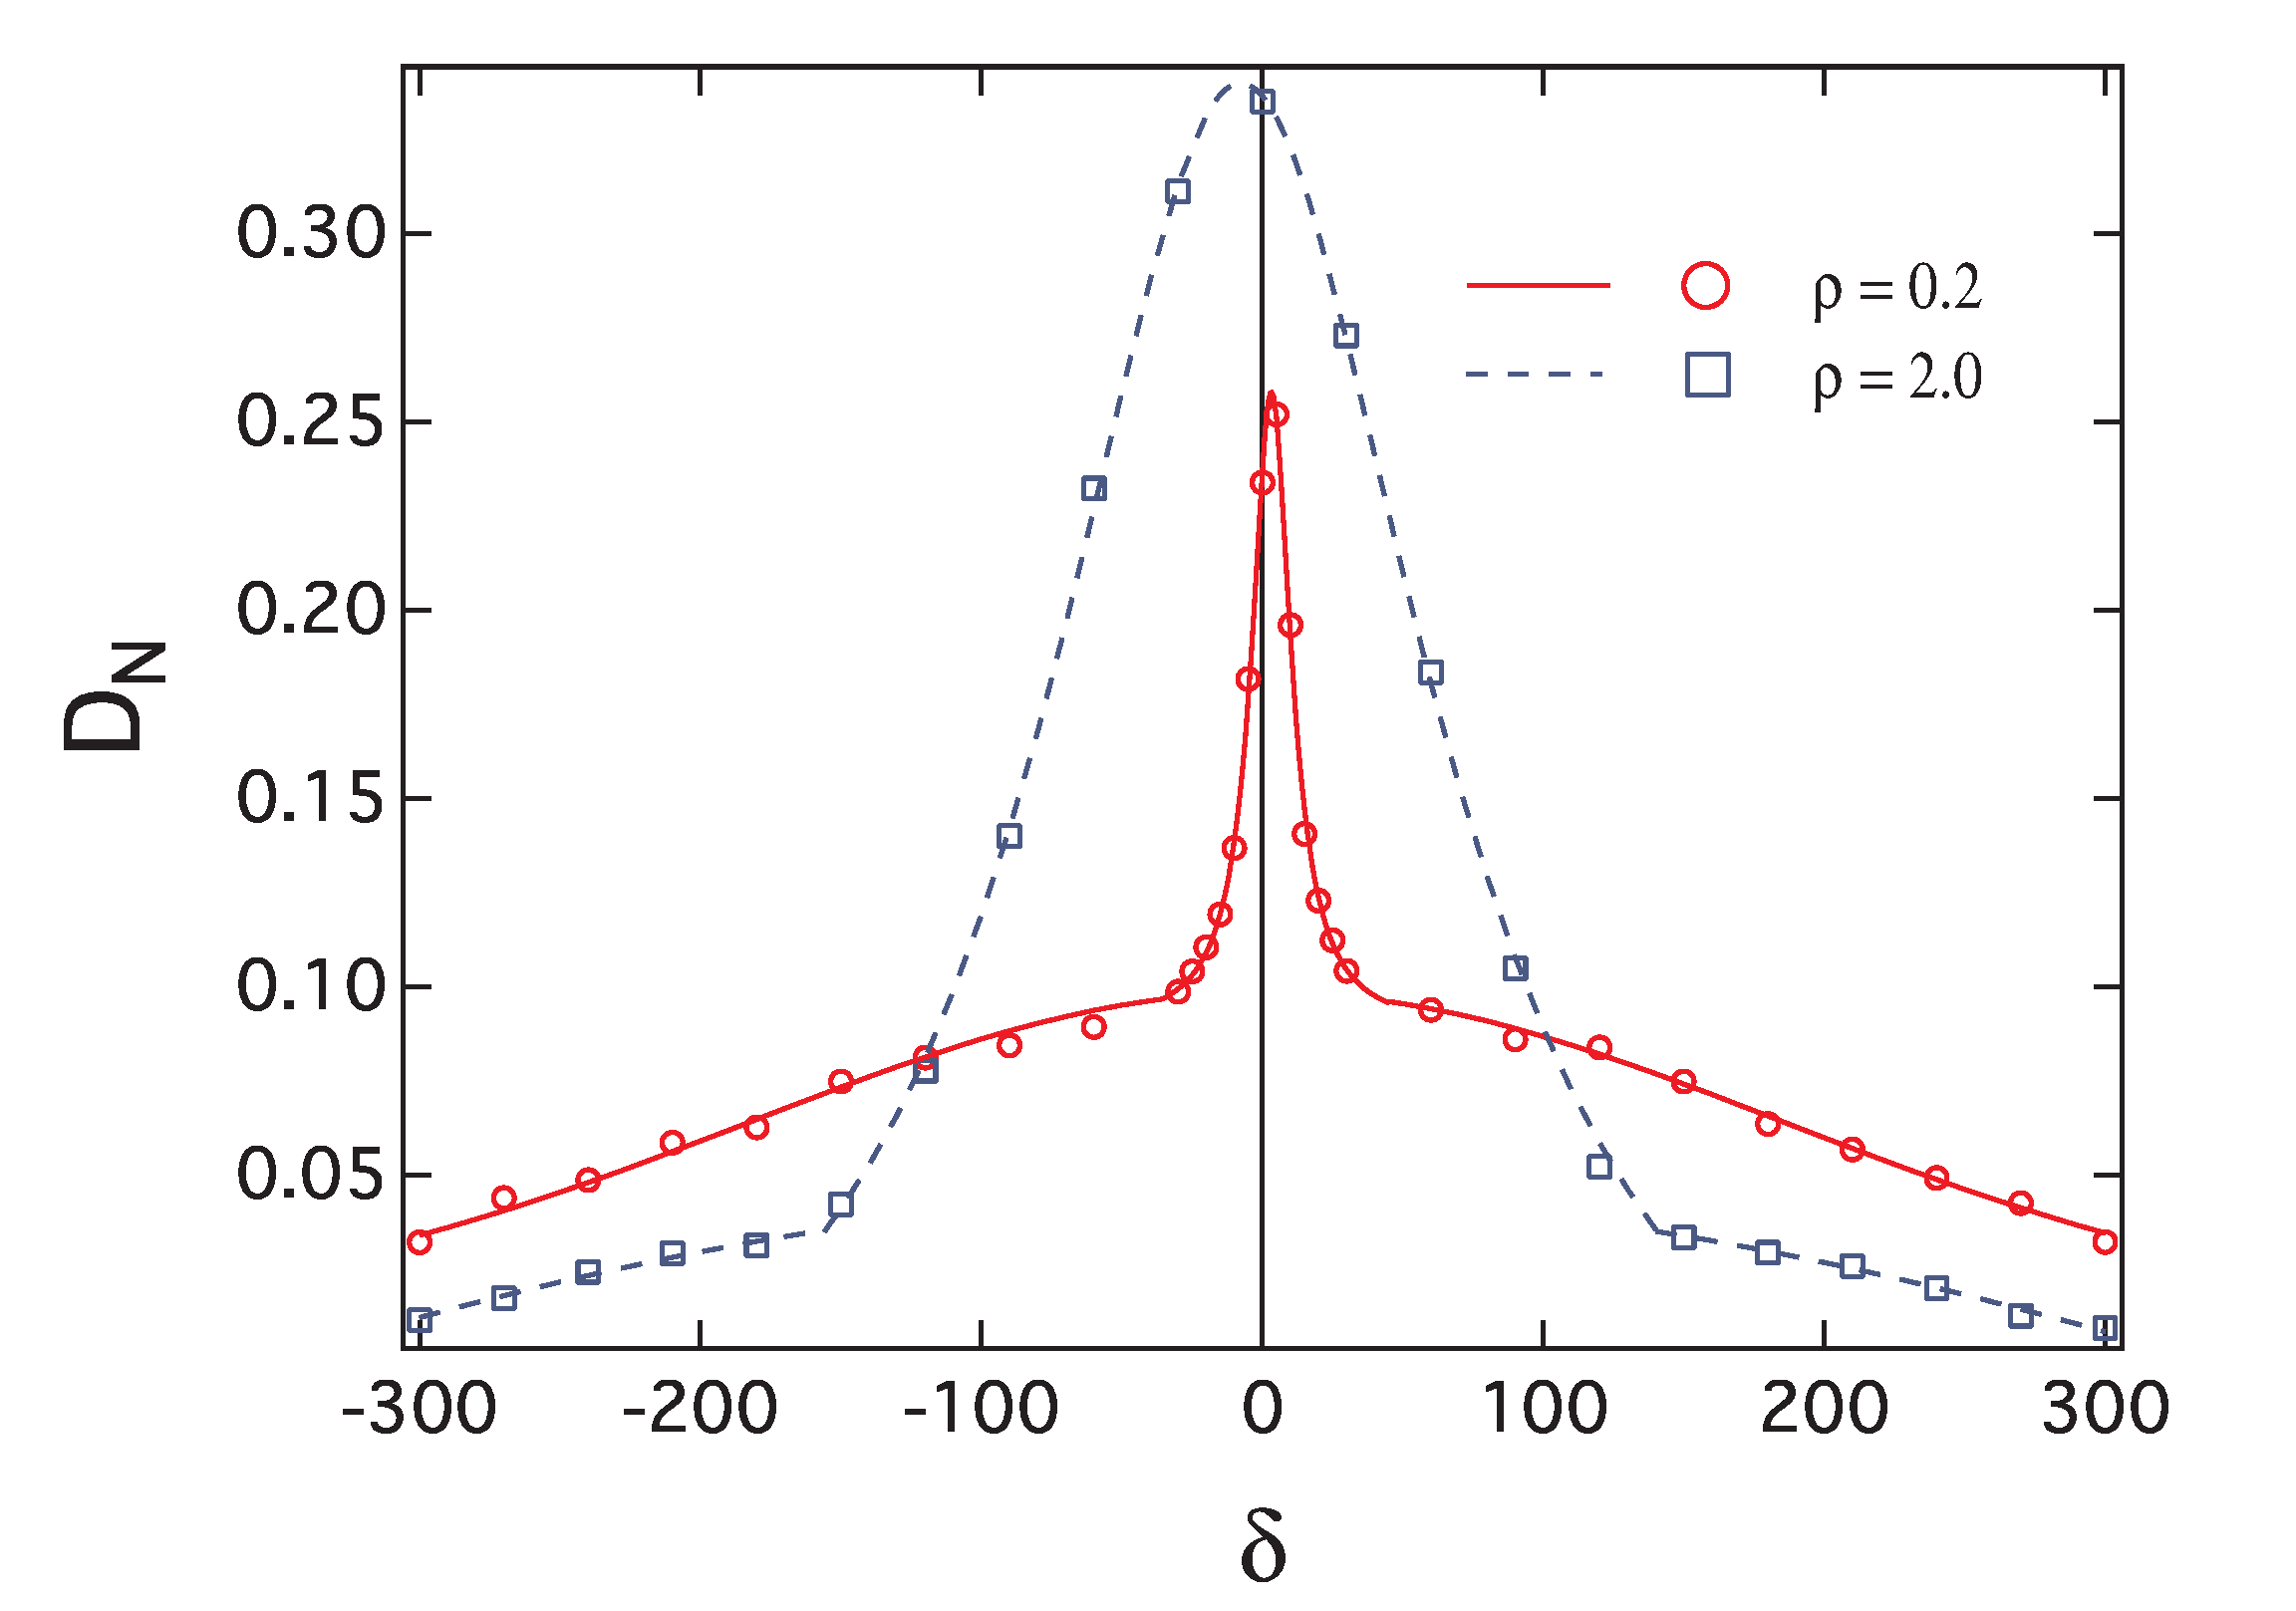
\includegraphics[width=\textwidth]{DICKE.pdf}
\end{center}
\caption{Optical thickness $D_N$ versus detuning $\delta$ in two samples with different densities but the same number of atoms $N=256$. The thickness of the disk is $h=5$ (red circles) and $0.5$ (blue boxes), respectively. The lines are fitted Lorentzian in the peak regions and Gaussian in the side-wings. In both cases the rms velocity of the atoms is $u=500$, and the radius of the disk is the usual $R=\sqrt{256/\pi}$. The collision radius of an atom is $r_a=0.01$, so atom-atom collisions are very rare.}
\label{DICKE}
\end{figure}

As shown in Fig.~\ref{DICKE},  in a dilute gas ($\rho =0.2$), a sharp Lorentzian peak arises near resonance over the base of a Gaussian profile due to inhomogeneous broadening. This is typical of Dicke narrowing. Note that in Sec.~\ref{SMAG} we also have a narrowing effect on the lineshape from collisions. However, what we observed is more like a continuous transition from a Gaussian to a Lorentzian, not an abrupt Lorentzian peak over a Gaussian base. We surmise that here the appearance of a Dicke narrowed spectrum does not result solely from collisions; in order to produce the final lineshape, dipole-dipole interactions (i.e. cooperative effects) must also be present.

In the high density regime ($\rho =2$), the spectrum is still composed of two parts: Gaussian in the side wings and Lorentzian at the center. However, the central peak, presumable a vestige of Dicke narrowing, is remarkably broadened even though the collision rate is much higher than for the density $\rho =0.2$.

\begin{figure}[h!]
\begin{center}
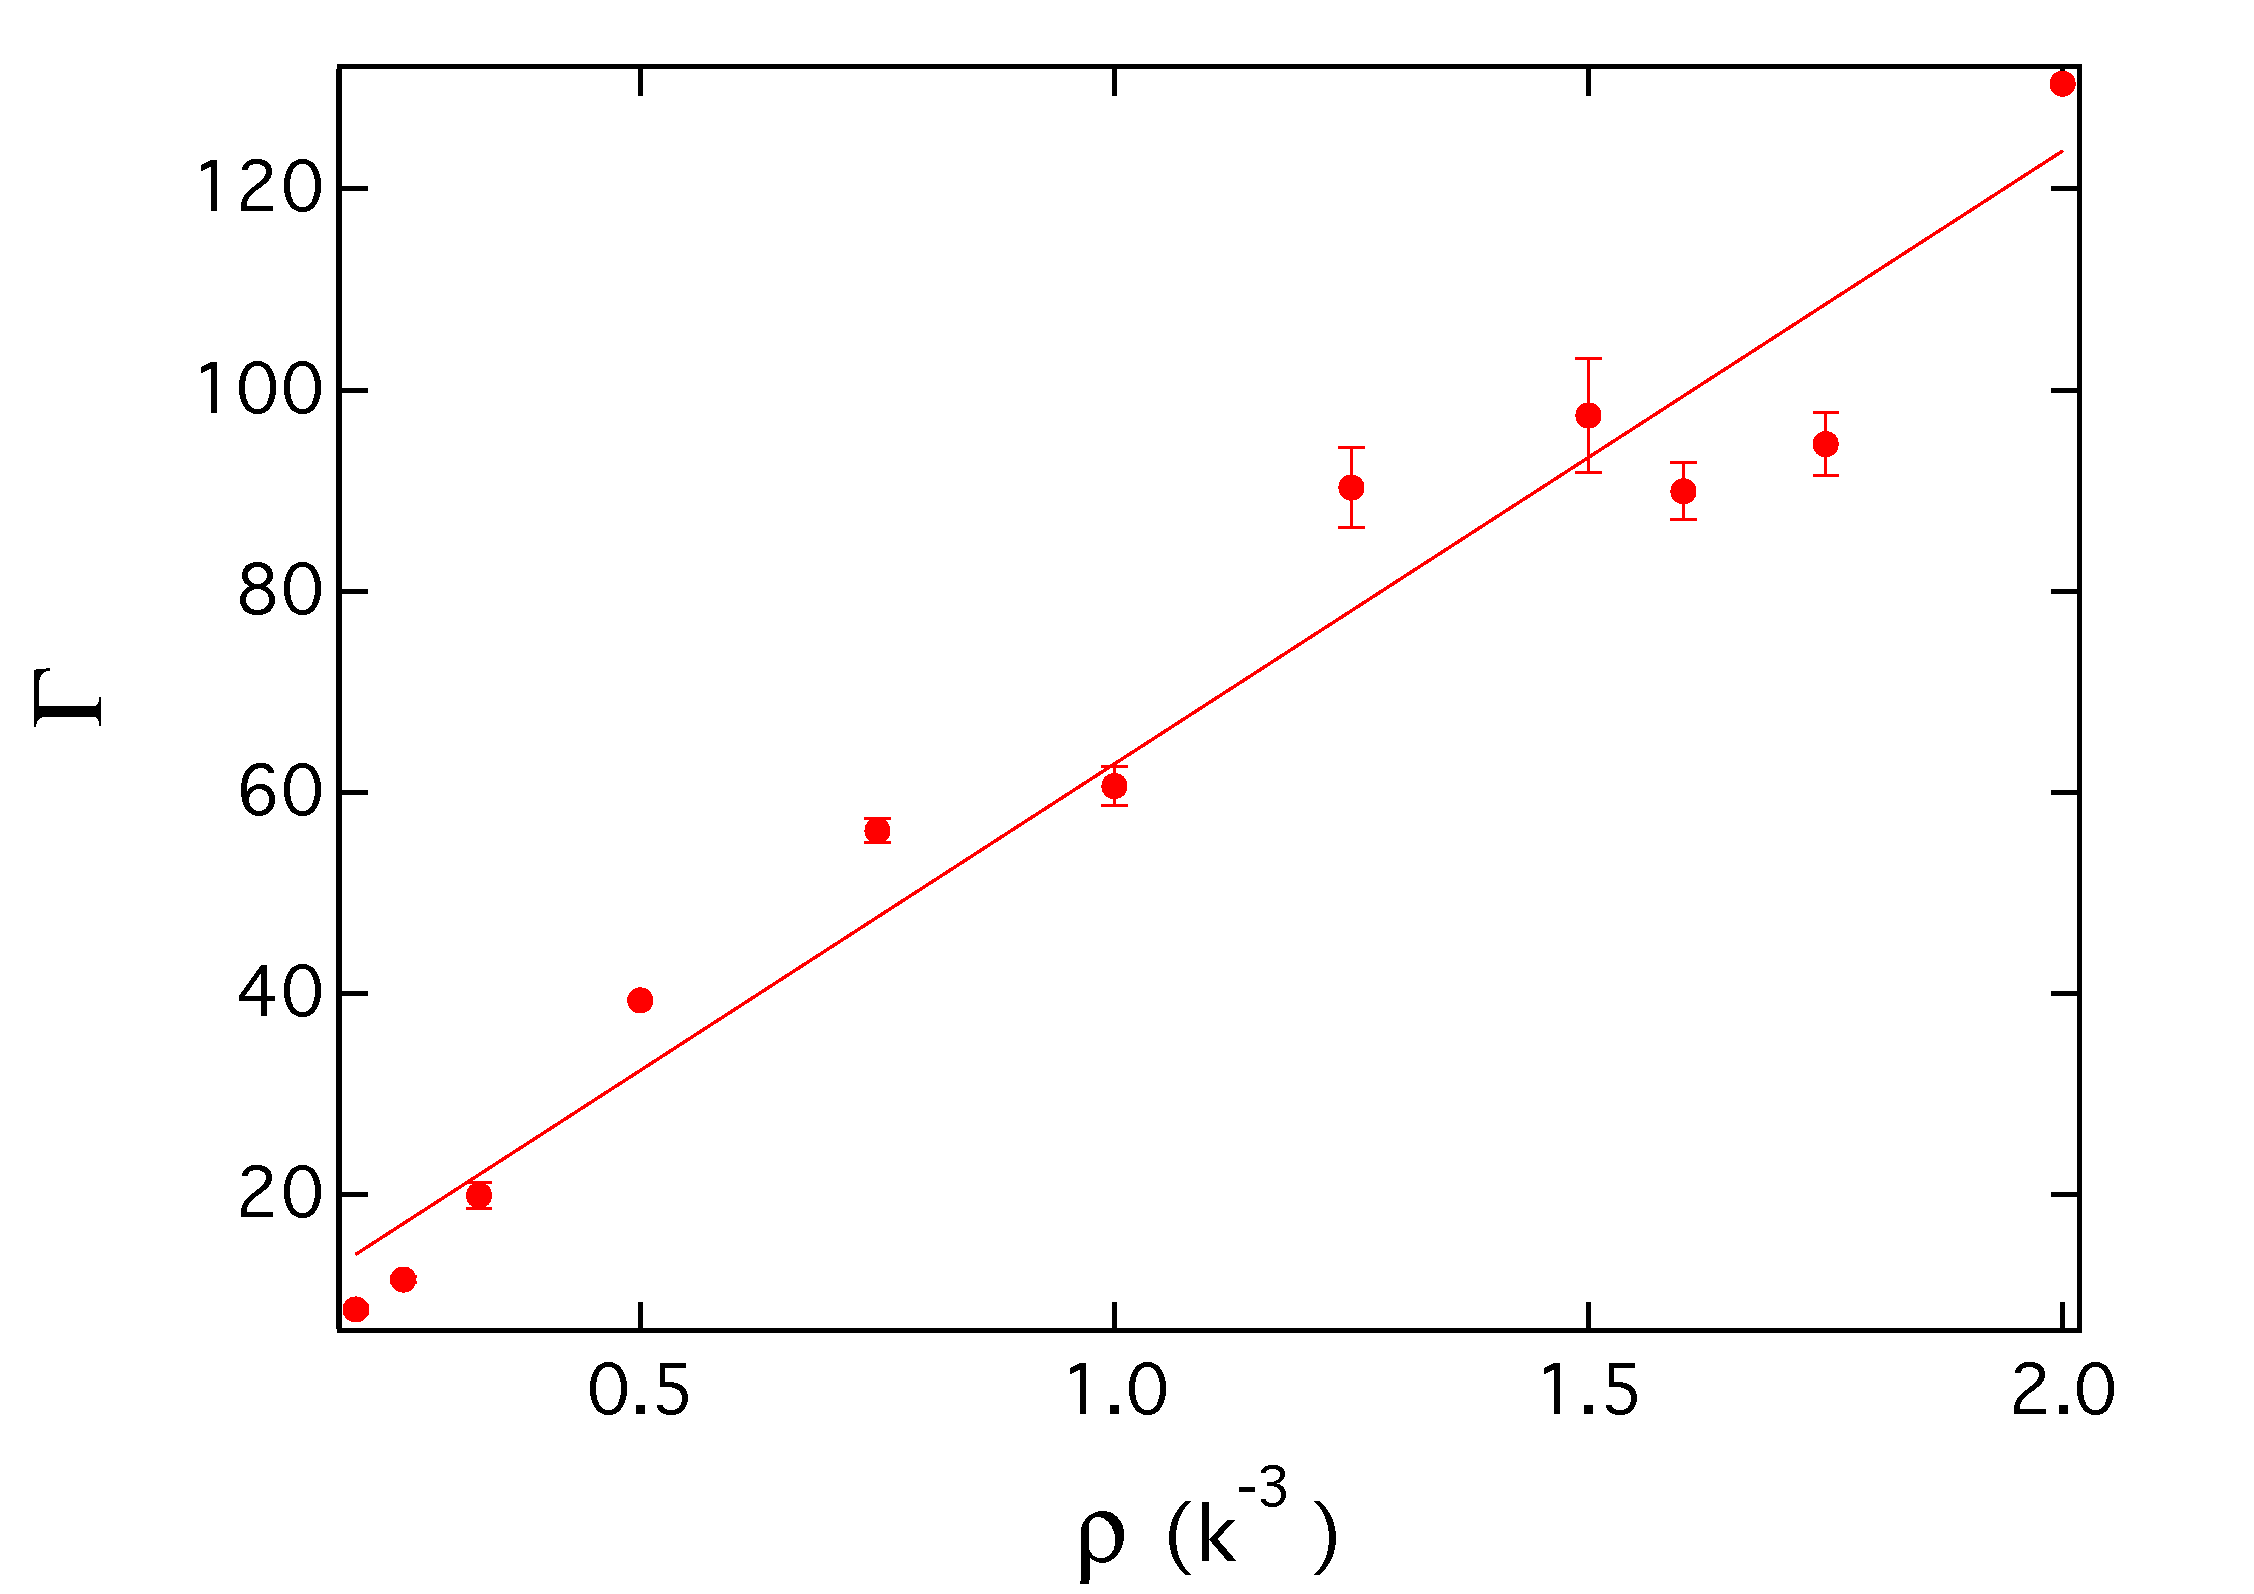
\includegraphics[width=\textwidth]{FWHM.pdf}
\end{center}
\caption{$\Gamma$ (the ratio of FWHM of the Lorentzian peak to $\gamma$) vs.\ density $\rho$ for the fixed number of atoms $N=256$. The density is changed by varying the thickness of the disk with the usual area $A=256$. As before, the motional broadening is specified by $u=500$. The collision radius is $r_a=0.01$, so atom-atom collisions are rare.}
\label{FWHM}
\end{figure}

Let us finally consider Fig.~\ref{FWHM}, which presents the width of the central peak as a function of the density of the gas. The width is obtained as the FWHM of the fitted Lorentzen peak. Recall the results we obtained in Sec.~\ref{SMAG}, without the dipole-dipole interactions, that a higher frequency of either atom-wall collisions or atom-atom collisions would narrow the lineshape. As increasing density in Fig.~\ref{FWHM} implies an increasing collision rate, the behavior of the linewidth is opposite to what one would expect for Dicke narrowing. Evidently, the width of the center peak of the spectrum keeps increasing because of the dipole-dipole interactions as the density goes up.  We surmise that this broadening is a cooperative effect due to rescattering of light between the atoms.

\chapter{Concluding Remarks}
For stationary atoms, an analytical calculation of radiated fields is feasible in simple cases such as a single atom, two atoms, and a non-cooperative Gaussian sample. We have derived explicit expressions for the total radiated power in these cases. The difference between a continuous medium and a sample of discrete non-interacting atoms touches on some fundamental problems in the traditional optics, which is essentially a mean-field theory.

We have carried out simulations for stationary atoms with the dipole-dipole interactions taken into account. A comparison of the total radiated power with independent atoms has revealed the presence of cooperative effects. We also note that the shift of the atomic resonance line in the simulations is not compatible with the conventional wisdom about local-field corrections.

We incorporated atomic motion, including various collisions, in our classical-electrodynamics simulations of light propagation in a dense gas sample. The simulations with atomic motion not only qualitatively reproduce the same results as we find for stationary atoms with a simple model of inhomogeneous broadening, such as collective Lamb shift, but also demonstrate new spectral features that result from interplay between Dicke narrowing and cooperative effects.

At this point it is becoming obvious that we have only seen the tip of the iceberg. 
References~\cite{PhysRevLett.112.113603} and~\cite{Javanainen:16} increasingly insistently promote the idea that the usual electrodynamics of polarizable media may fail qualitatively in the kind of cold dense gases brought to us by laser cooling and evaporative cooling. Conversely, it is becoming clear that the quintessential cooperative Lamb shift in a slab geometry can be explained as a near-trivial consequence of classical optics. Let us bring in another thought directly related to the present thesis: We have seen line broadening with increasing atom density in our simulations, evidently as a result of cooperative atom-atom interactions. Now, conventional wisdom says that resonance lines {\em do\/} broaden with atom density; it is called collision broadening. Could it be that collision broadening is actually a cooperative effect due to dipole-dipole interactions?

We conclude with the following theses: The molecular basis of the electrodynamics of material samples is probably not as well understood as we have thought until now. Numerical simulations on massive computer clusters are a new theoretical method to address this problem area, and the progress in experimental techniques with cold atoms will eventually enable decisive experiments. Classical electrodynamics, a field whose fundamentals were seemingly set in stone well over a century ago, is due for new developments.





\bibliography{bib_summary}



% appendices: we put them after the references in what ever order
% we prefer
%\input{appendices/dsmethod.tex}
\end{document}

